

\begin{figure}[H]
\subbottom[]{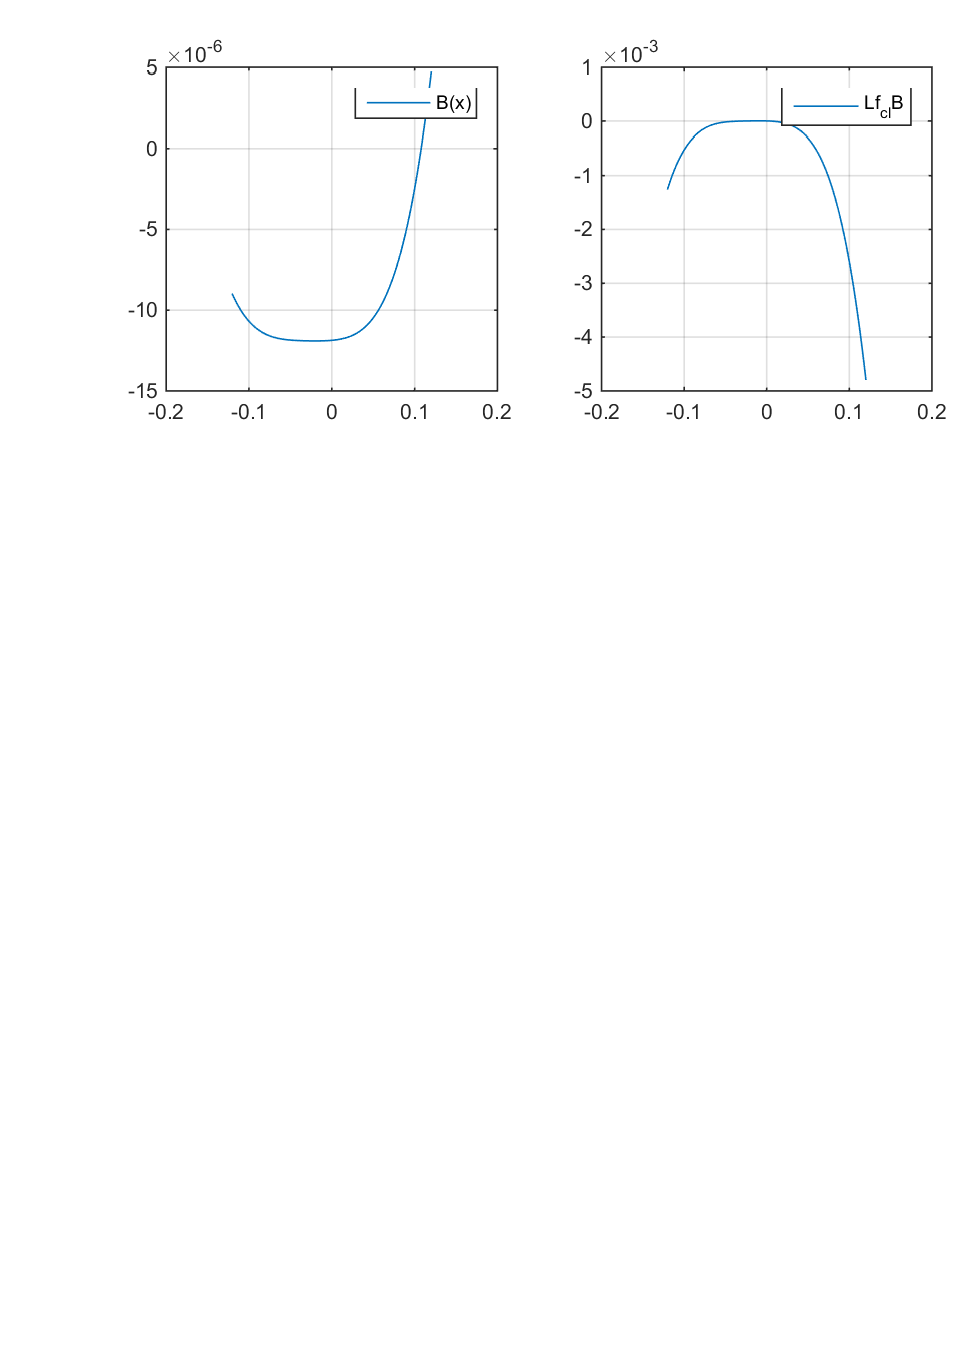
\includegraphics[width=0.5\textwidth]{barrier1.pdf}}%
\subbottom[]{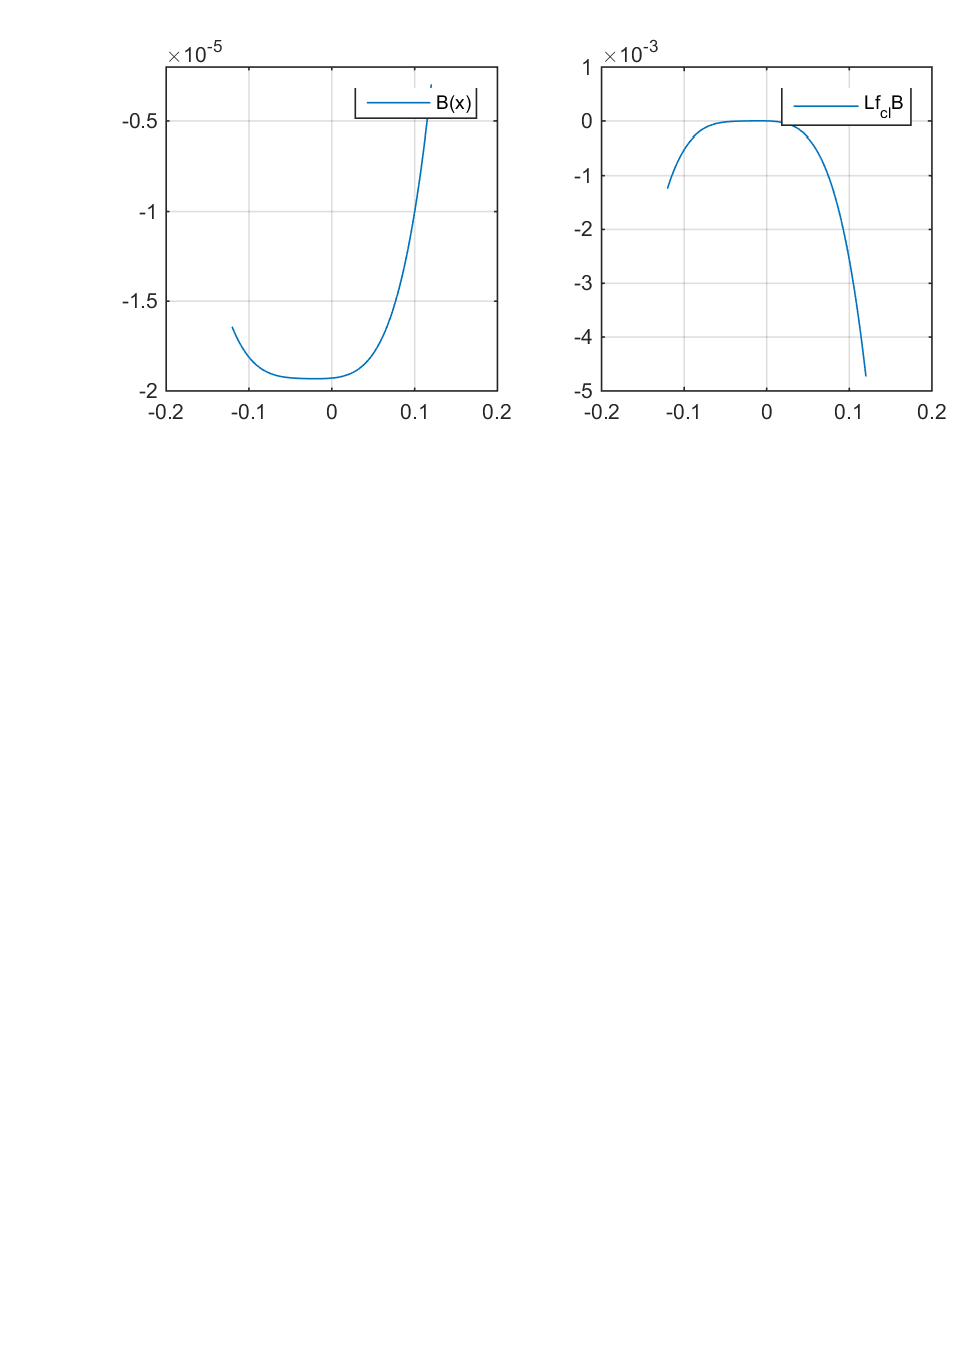
\includegraphics[width=0.5\textwidth]{barrier2.pdf}}%
\hspace{1mm}
\subbottom[]{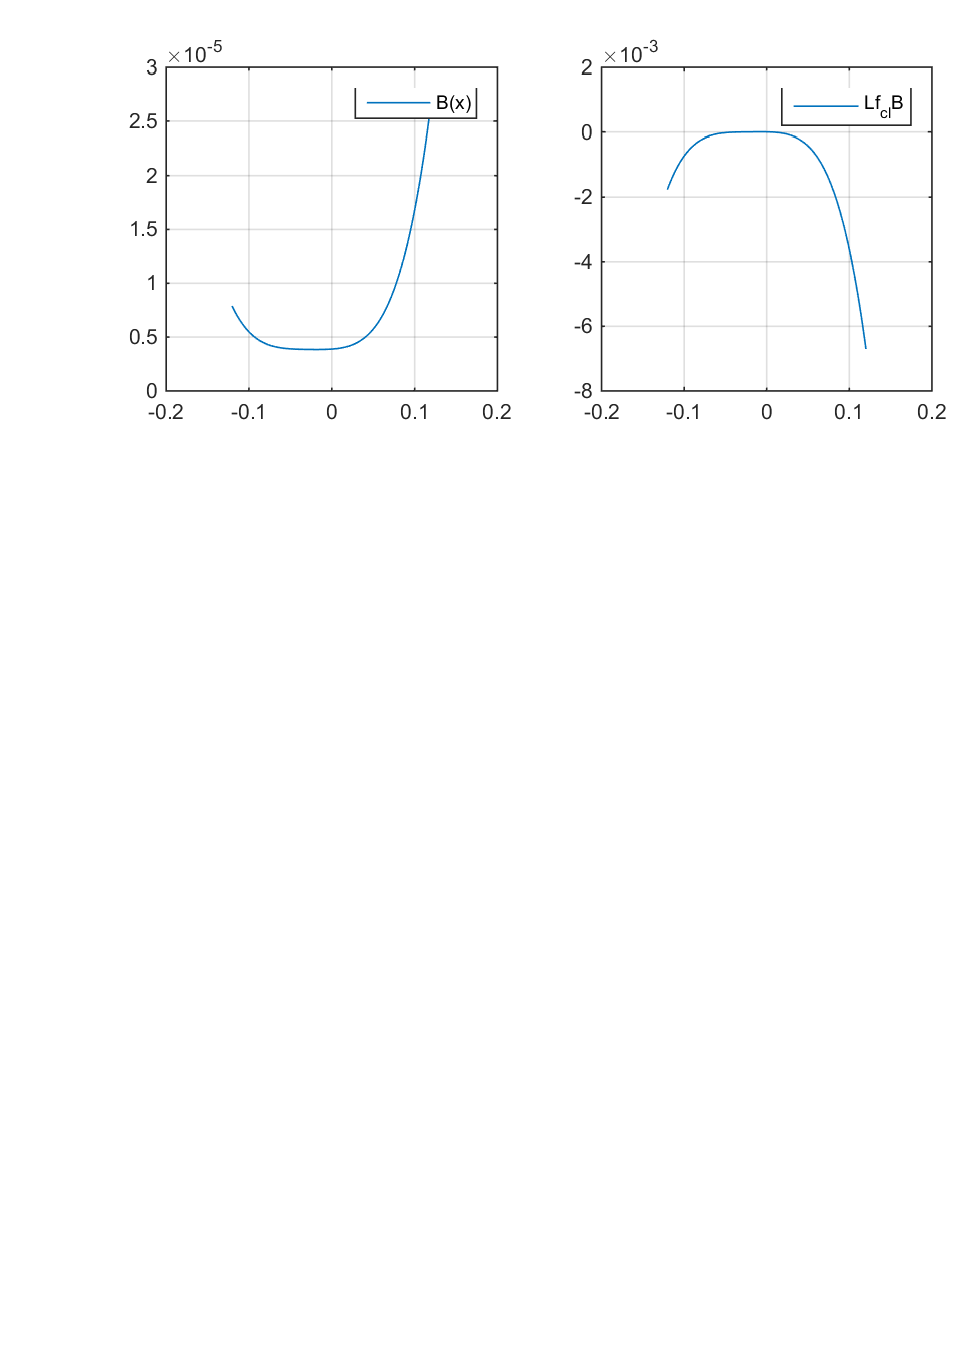
\includegraphics[width=0.5\textwidth]{barrier3.pdf}}%
\subbottom[]{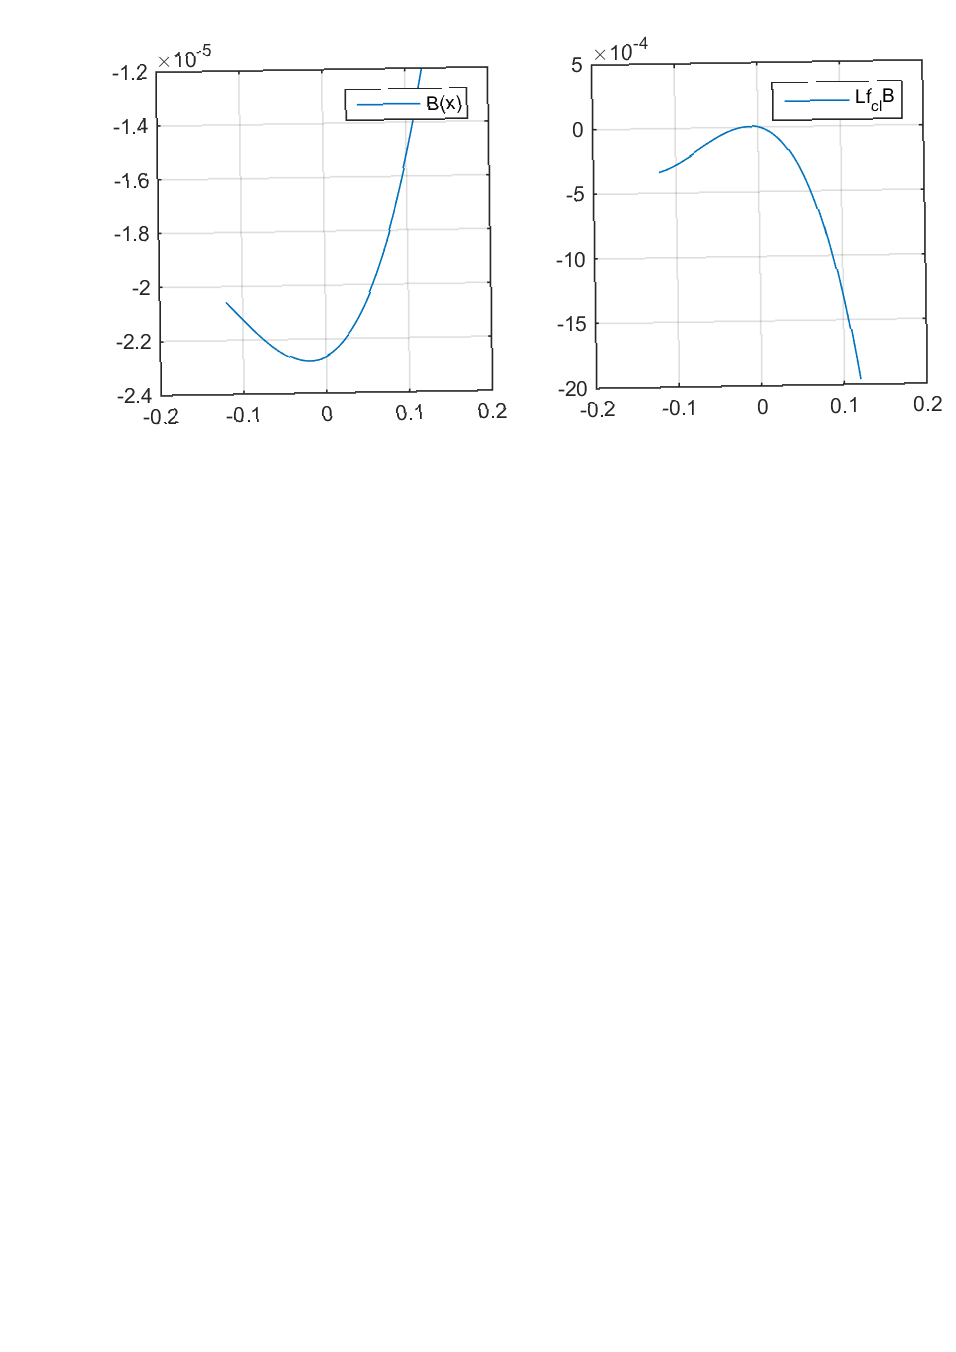
\includegraphics[width=0.5\textwidth]{barrier4.pdf}}%
\caption{Examples of generated barrier functions with different combinations of monomial degrees.}
\end{figure}

\newpage
\section{New tests with SOSTOOLS}
Different definitions of the sets $\mathcal{X}$, $\mathcal{X}_0$ and $\mathcal{X}_u$ are tested, presented in \autoref{fig:intervals_for_sos1}, \ref{fig:intervals_for_sos2} and \ref{fig:intervals_for_sos3}, with varying monomial degrees, and barrier dependency (on $x_1$ alone or on both $x_1$ and $x_{ref}$).

Testing with $\Delta=1$e-4 and $\epsilon=1$e-10. All inequalities are set up as in \autoref{eq:barrier_constraints_putinar}.

Tried to change unit of state from [m] to [cm] (i.e. multiplied limits with scaling factor):
\begin{lstlisting}[language=matlab]
% scaling factor = 1 for [meter], or 100 for [cm]
scaling = 100;

% Distance reference should keep to the unsafe region
delta = 1e-4*scaling;

% Distance which the unsafe region is allowed to deviate from the desired zero
% level set specified by the g(x) defining Xu
epsilon = 1e-10*scaling;

% Set upper and lower limits for the set intervals X, Xu and X0
Xmax = 0.1*scaling;
Xmin = -0.1*scaling;
Xumax = Xmax;
Xumin = 0.05*scaling;
X0max = Xumin-delta;
X0min = Xmin;
\end{lstlisting}
but this gives more or less the same solution, change is leading coefficient increased by an order of degree.

\subsection{Case 1}\label{case1}
\begin{figure}[htbp]
\centering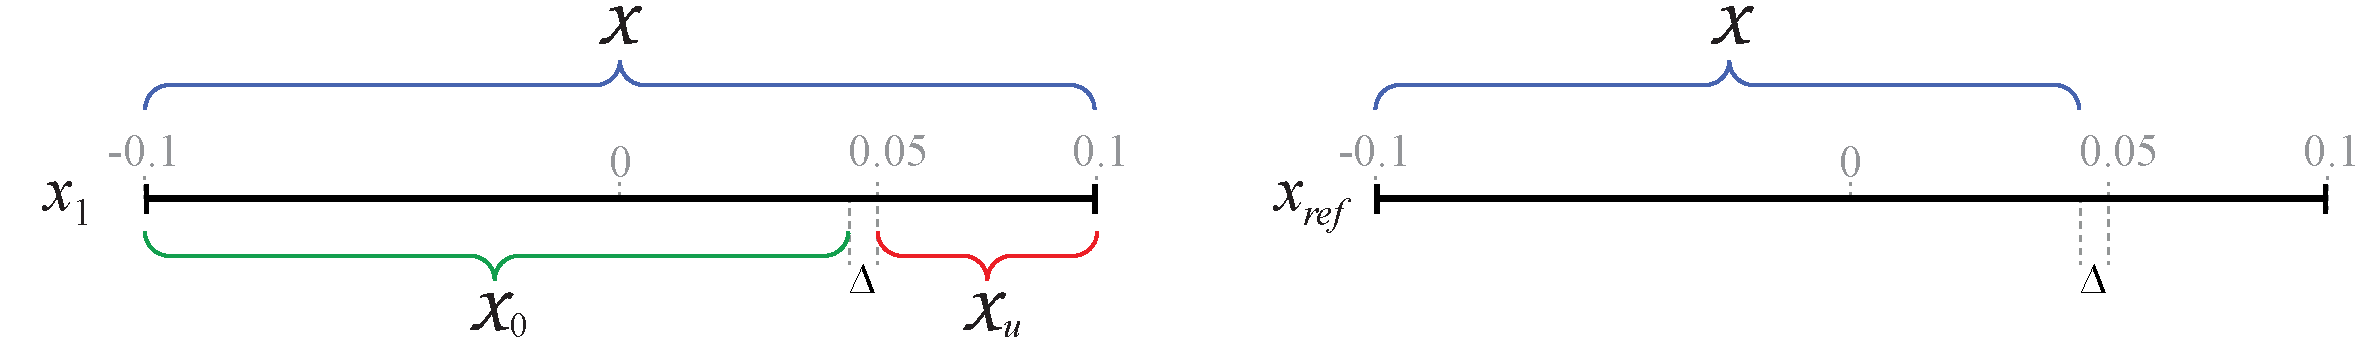
\includegraphics[width=\textwidth]{intervals_for_sos1.pdf}
\caption{Only the set $\mathcal{X}$ is defined by both $x_1$ and $x_{ref}$, while $\mathcal{X}_0$ and $\mathcal{X}_u$ are independent of $x_{ref}$.}
\label{fig:intervals_for_sos1}
\end{figure}

With sets defined as in \autoref{fig:intervals_for_sos1}:
\begin{subequations}\label{eq:sets_case1}
\begin{align}
\mathcal{X} &= \begin{bmatrix} -0.1 & 0.1\end{bmatrix} \times \begin{bmatrix} -0.1 & 0.05-\Delta\end{bmatrix}\\
\mathcal{X}_u &= \begin{bmatrix} 0.05 & 0.1\end{bmatrix} \times \mathbb{R}\\
\mathcal{X}_0 &= \begin{bmatrix} -0.1 & 0.05-\Delta\end{bmatrix} \times \mathbb{R}
\end{align}
\end{subequations}
Letting $B(x_1,x_{ref})$, degree 0:4, gives solution with \texttt{feasratio=1}, while \texttt{numerr=1} in every case (however \texttt{res.norm=8e-7}) and leading term coefficient 1e-4. Plot of $B(x)$ looks "okay" (looks like function of equally much both states). Changing to $B(x_1)$ gives more or less the same except leading term coefficient 3e-9.

In the figures datatips are marking (as close as possible) the zero level set.

\begin{figure}[htbp]
\centering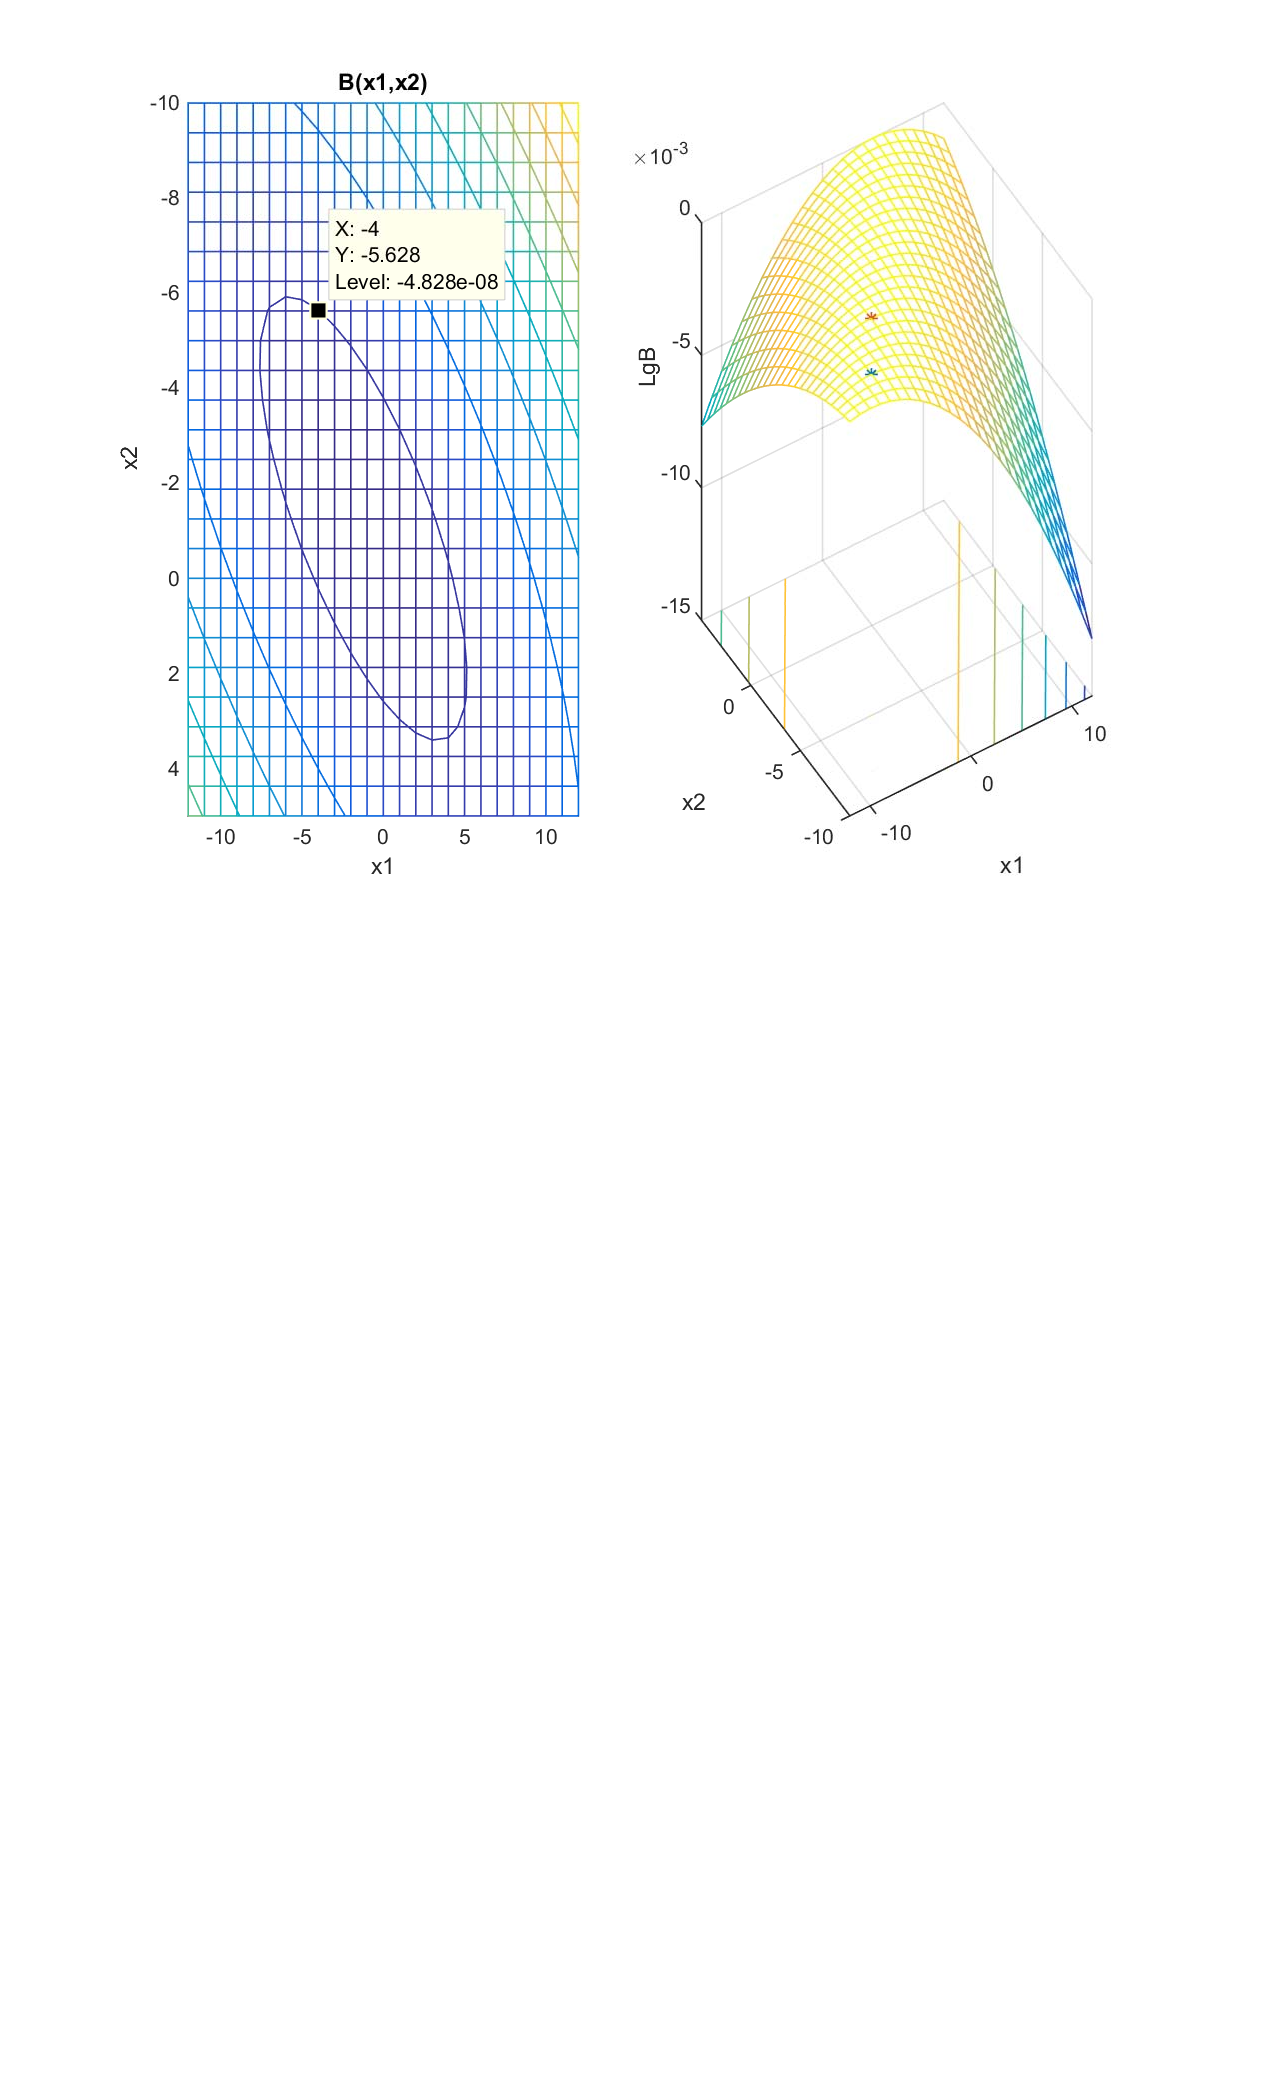
\includegraphics[width=0.7\textwidth]{Bxtilde1.pdf}
\caption{(\Autoref{case1}) Test with $B(x_1,x_{ref})$ of degree 0:2, and maximum monomial degrees $q_{X1}=2$, $q_{X2}=3$, $q_{Xu}=2$, $q_{X0}=4$. Not really a solution: \texttt{feasratio=0.6399}, \texttt{numerr=0}, \texttt{res.norm=4e-9} but leading term coefficient 1e-7.}
\label{fig:Bxtilde1}
\end{figure}

\begin{figure}[htbp]
\centering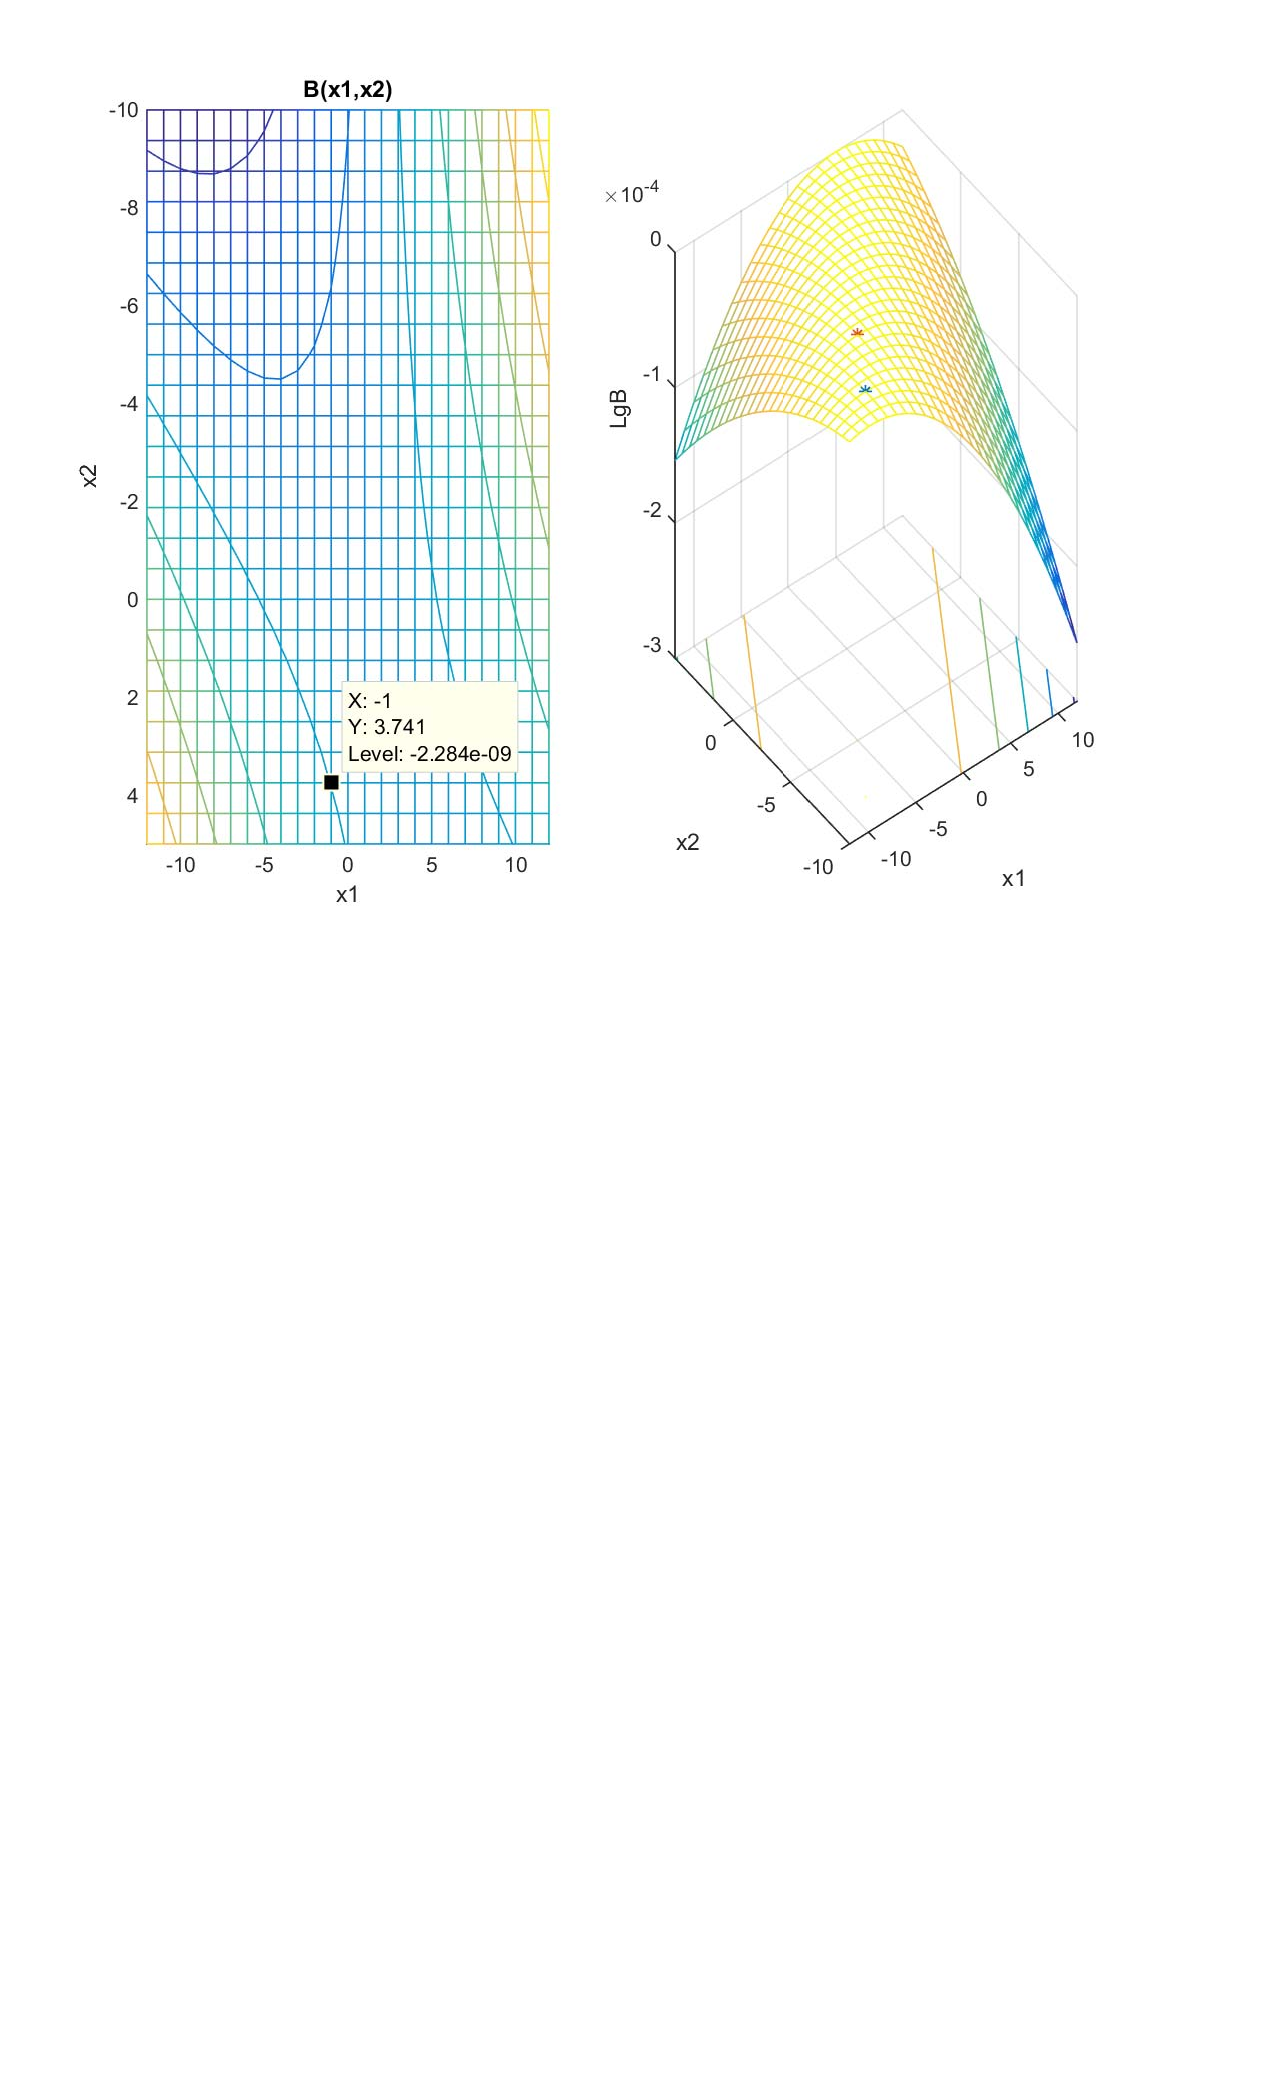
\includegraphics[width=0.7\textwidth]{Bxtilde2.pdf}
\caption{(\Autoref{case1}) Same as in \autoref{fig:Bxtilde1} but with all monomial degrees 0:2. Not really a solution: \texttt{feasratio=0.9712}, \texttt{numerr=0}, \texttt{res.norm=1e-9} but leading term coefficient 2e-9.}
\label{fig:Bxtilde2}
\end{figure}

\begin{figure}[htbp]
\centering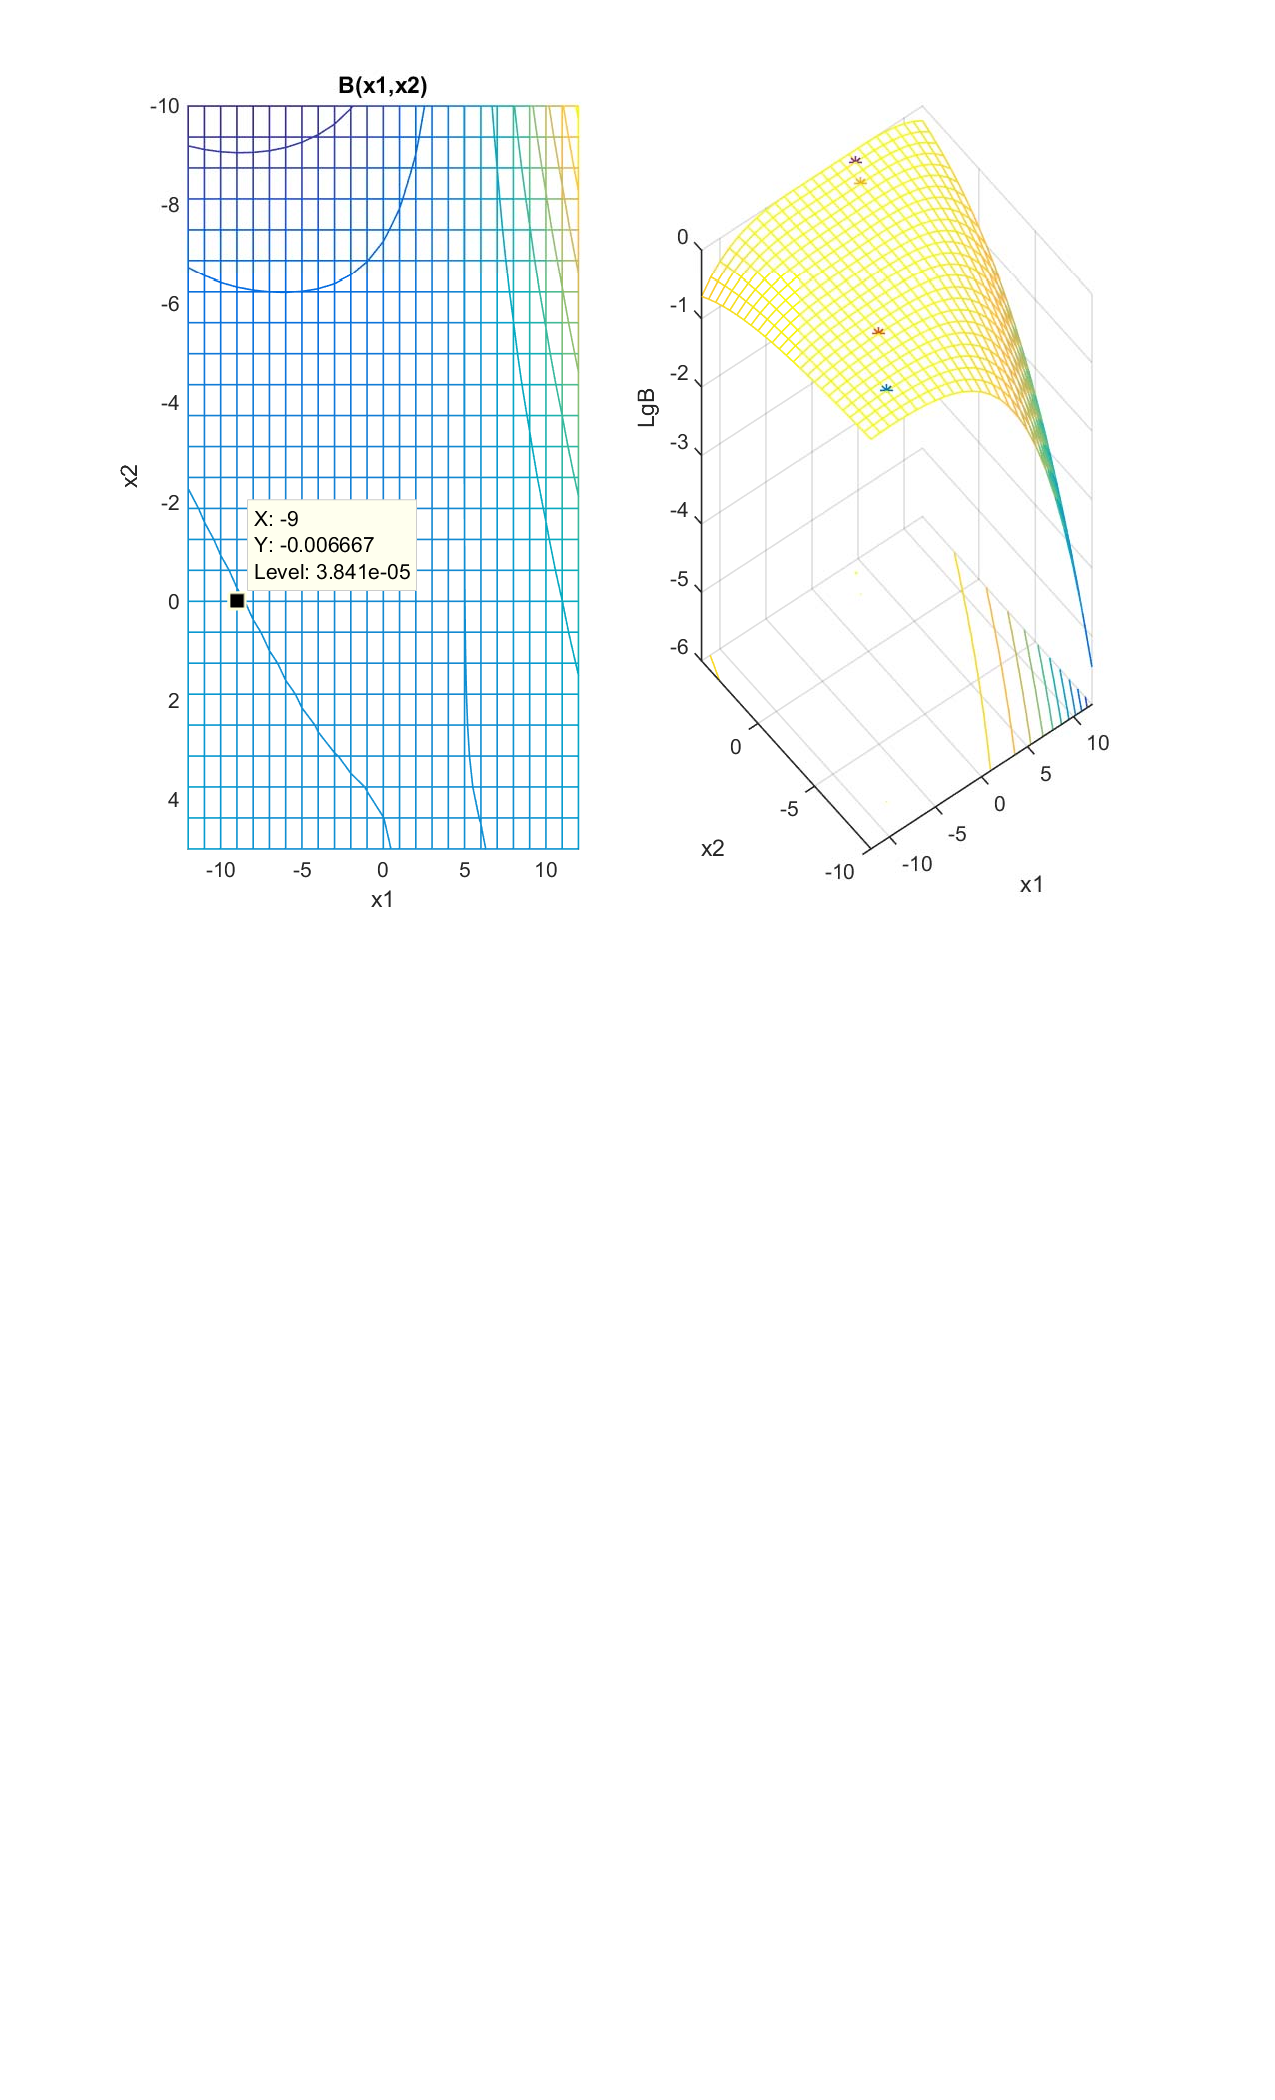
\includegraphics[width=0.7\textwidth]{Bxtilde3.pdf}
\caption{(\Autoref{case1}) Same as in \autoref{fig:Bxtilde2} but with $B(x)$ monomial degree 0:4. Not really a solution: \texttt{feasratio=0.9992}, \texttt{numerr=0}, \texttt{res.norm=2e-7} but leading term coefficient 6e-8.}
\label{fig:Bxtilde3}
\end{figure}

\newpage
\subsection{Case 2}\label{case2}
\begin{figure}[htbp]
\centering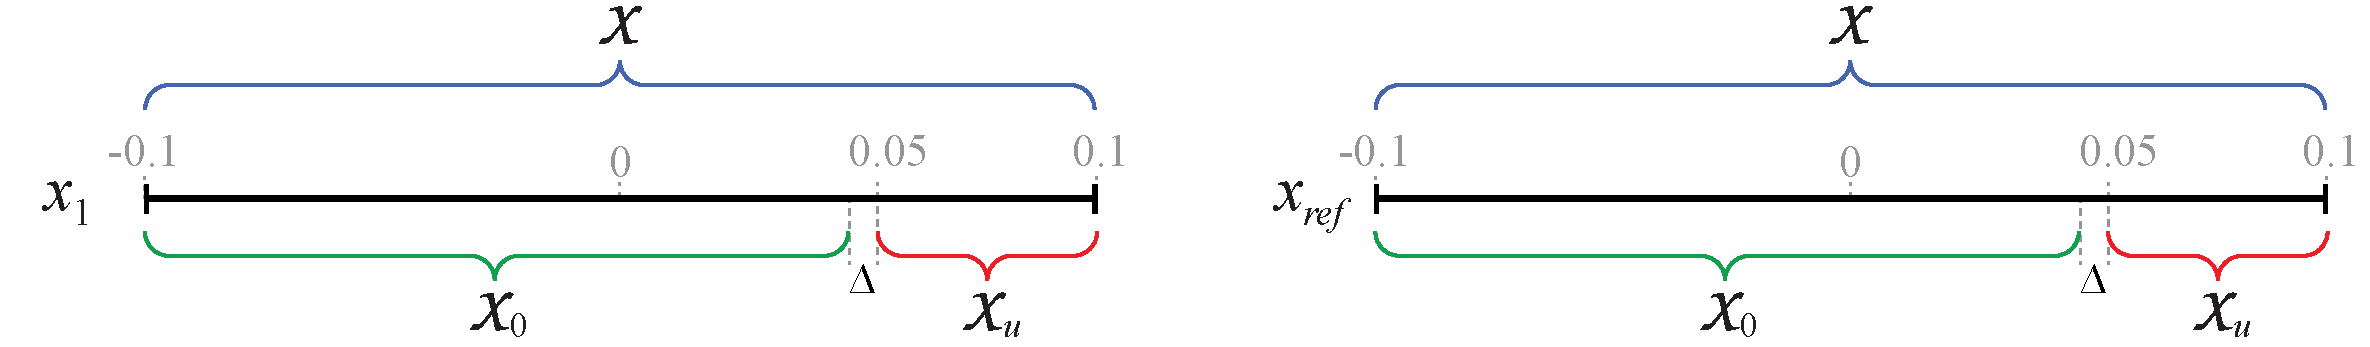
\includegraphics[width=\textwidth]{intervals_for_sos2.pdf}
\caption{All three sets are defined by both $x_1$ and $x_{ref}$, both defined in the same intervals (of the z-axis, corresponding to the slide axis).}
\label{fig:intervals_for_sos2}
\end{figure}
\begin{subequations}\label{eq:sets_case2}
With sets defined as in \autoref{fig:intervals_for_sos2}:
\begin{align}
	\mathcal{X} &= \begin{bmatrix} -0.1 & 0.1\end{bmatrix} \times \begin{bmatrix} -0.1 & 0.1\end{bmatrix}\\
	\mathcal{X}_u &= \begin{bmatrix} 0.05 & 0.1\end{bmatrix} \times \begin{bmatrix} 0.05 & 0.1\end{bmatrix}\\
	\mathcal{X}_0 &= \begin{bmatrix} -0.1 & 0.05-\Delta\end{bmatrix} \times \begin{bmatrix} -0.1 & 0.05-\Delta\end{bmatrix}
\end{align}
\end{subequations}
With this definition of the sets, the barrier certificate must be a function of both states: $B(x_1,x_{ref})$. Degree of barrier function tested with 0:2 and 0:4. Yields \texttt{feasratio=1}, \texttt{res.norm=8e-9}, leading coefficients approx 4e-4. However, plot reveals that $B(x)$ looks like it is "almost only" a function of $x_{ref}$ and not $x_1$ -- \textcolor{red}{why???}

Tried to test with the barrier certificate only a function of the robot position: $B(x_1)$: no solution (leding term coefficient 8e-9).

In general for all tests in this case \texttt{feasratio}$\approx 1$, while \texttt{numerr=1} in every case (however \texttt{res.norm} is in general of degree 1e-6 to 1e-9). Also blots of $B(x)$ all looks like it is "much more a function of" $x_{ref}$ than $x_1$, even when monomial degrees for $q$ polynomial-coefficients for $g(x_1)$ functions are set to be larger than those for the $g(x_{ref})$ functions.

%Examples in the figures below.

%\begin{figure}[h]
%\centering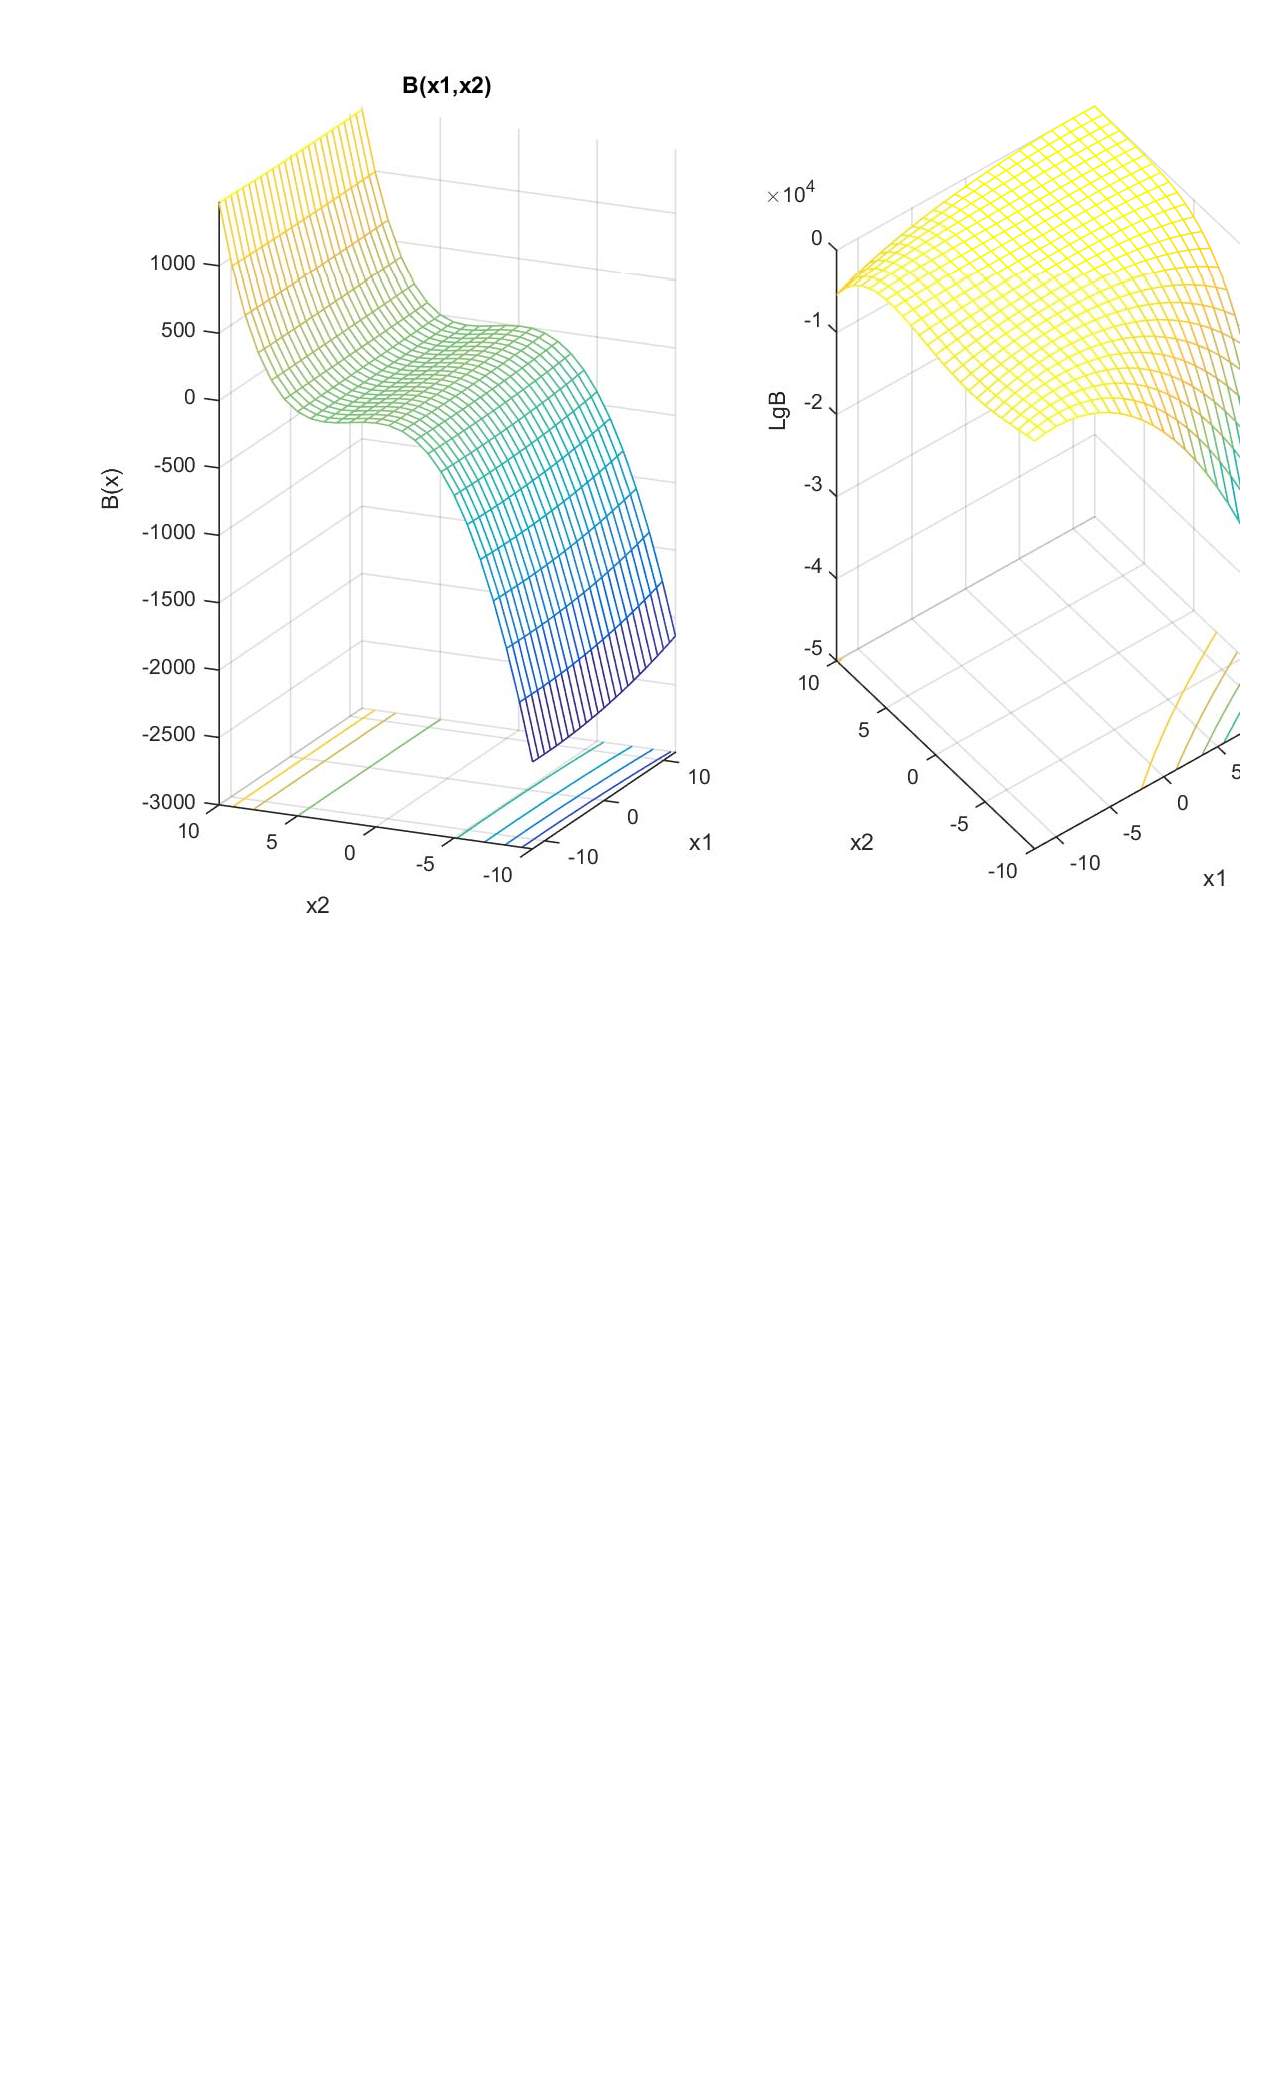
\includegraphics[width=0.7\textwidth]{Bxtilde4.pdf}
%\caption{(\Autoref{case2}) $B(x_1,x_{ref})$ of degree 0:4, all other monomials of degree 0:2. \texttt{feasratio=1}, \texttt{numerr=1}, \texttt{res.norm=8e-8}, leading term coefficient 4e-5.}
%\label{fig:Bxtilde4}
%\end{figure}
%\newpage
\subsection{Case 3}\label{case3}
\begin{figure}[htbp]
\centering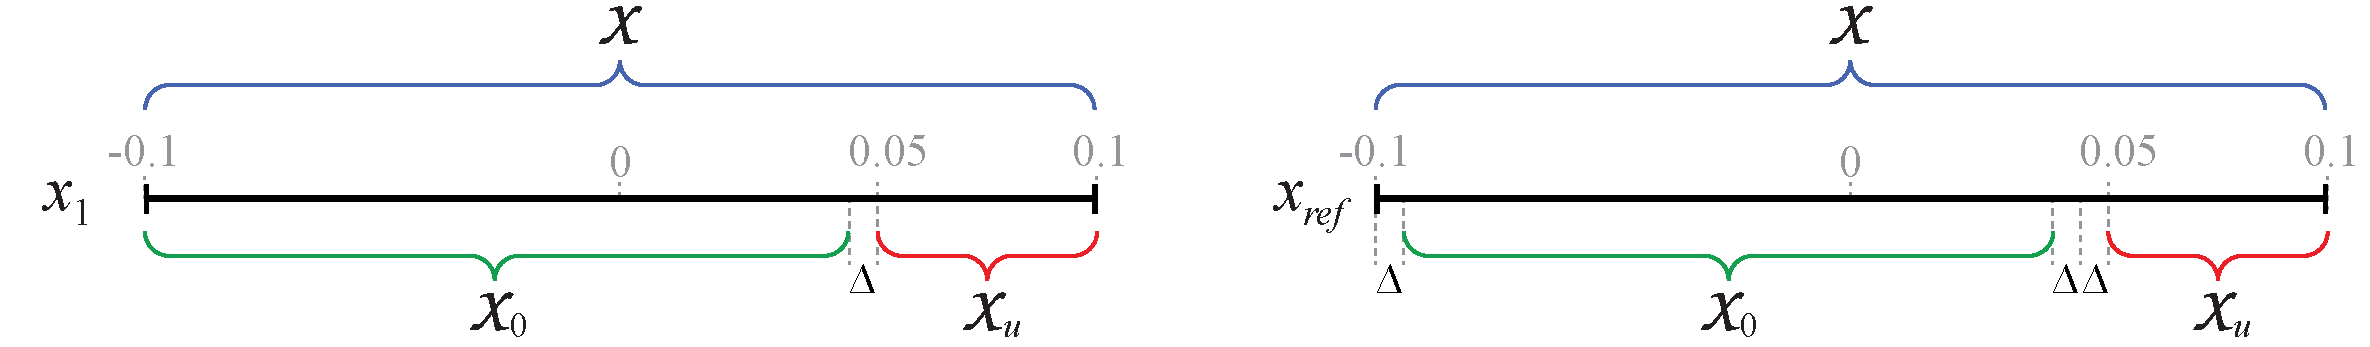
\includegraphics[width=\textwidth]{intervals_for_sos3.pdf}
\caption{All three sets are defined by both $x_1$ and $x_{ref}$, both defined in the same intervals except for $\mathcal{X}_0$ which has a smaller interval of allowed values.}
\label{fig:intervals_for_sos3}
\end{figure}
\begin{subequations}\label{eq:sets_case3}
With sets defined as in \autoref{fig:intervals_for_sos1}:
\begin{align}
	\mathcal{X} &= \begin{bmatrix} -0.1 & 0.1\end{bmatrix} \times \begin{bmatrix} -0.1 & 0.1\end{bmatrix}\\
	\mathcal{X}_u &= \begin{bmatrix} 0.05 & 0.1\end{bmatrix} \times \begin{bmatrix} 0.05 & 0.1\end{bmatrix}\\
	\mathcal{X}_0 &= \begin{bmatrix} -0.1 & 0.05-\Delta\end{bmatrix} \times \begin{bmatrix} -0.1+\Delta & 0.05-2\Delta\end{bmatrix}
\end{align}
\end{subequations}
Results are much the same as for case 2, generally \texttt{feasratio}$\approx 1$, while \texttt{numerr=1} in every case (however \texttt{res.norm} is in general of degree 1e-6 to 1e-9).

As seen from the figures below, again $B(x)$ looks like it is "mostly a function of" $x_{ref}$ and not so much $x_1$ (???)

\begin{figure}[h]
\centering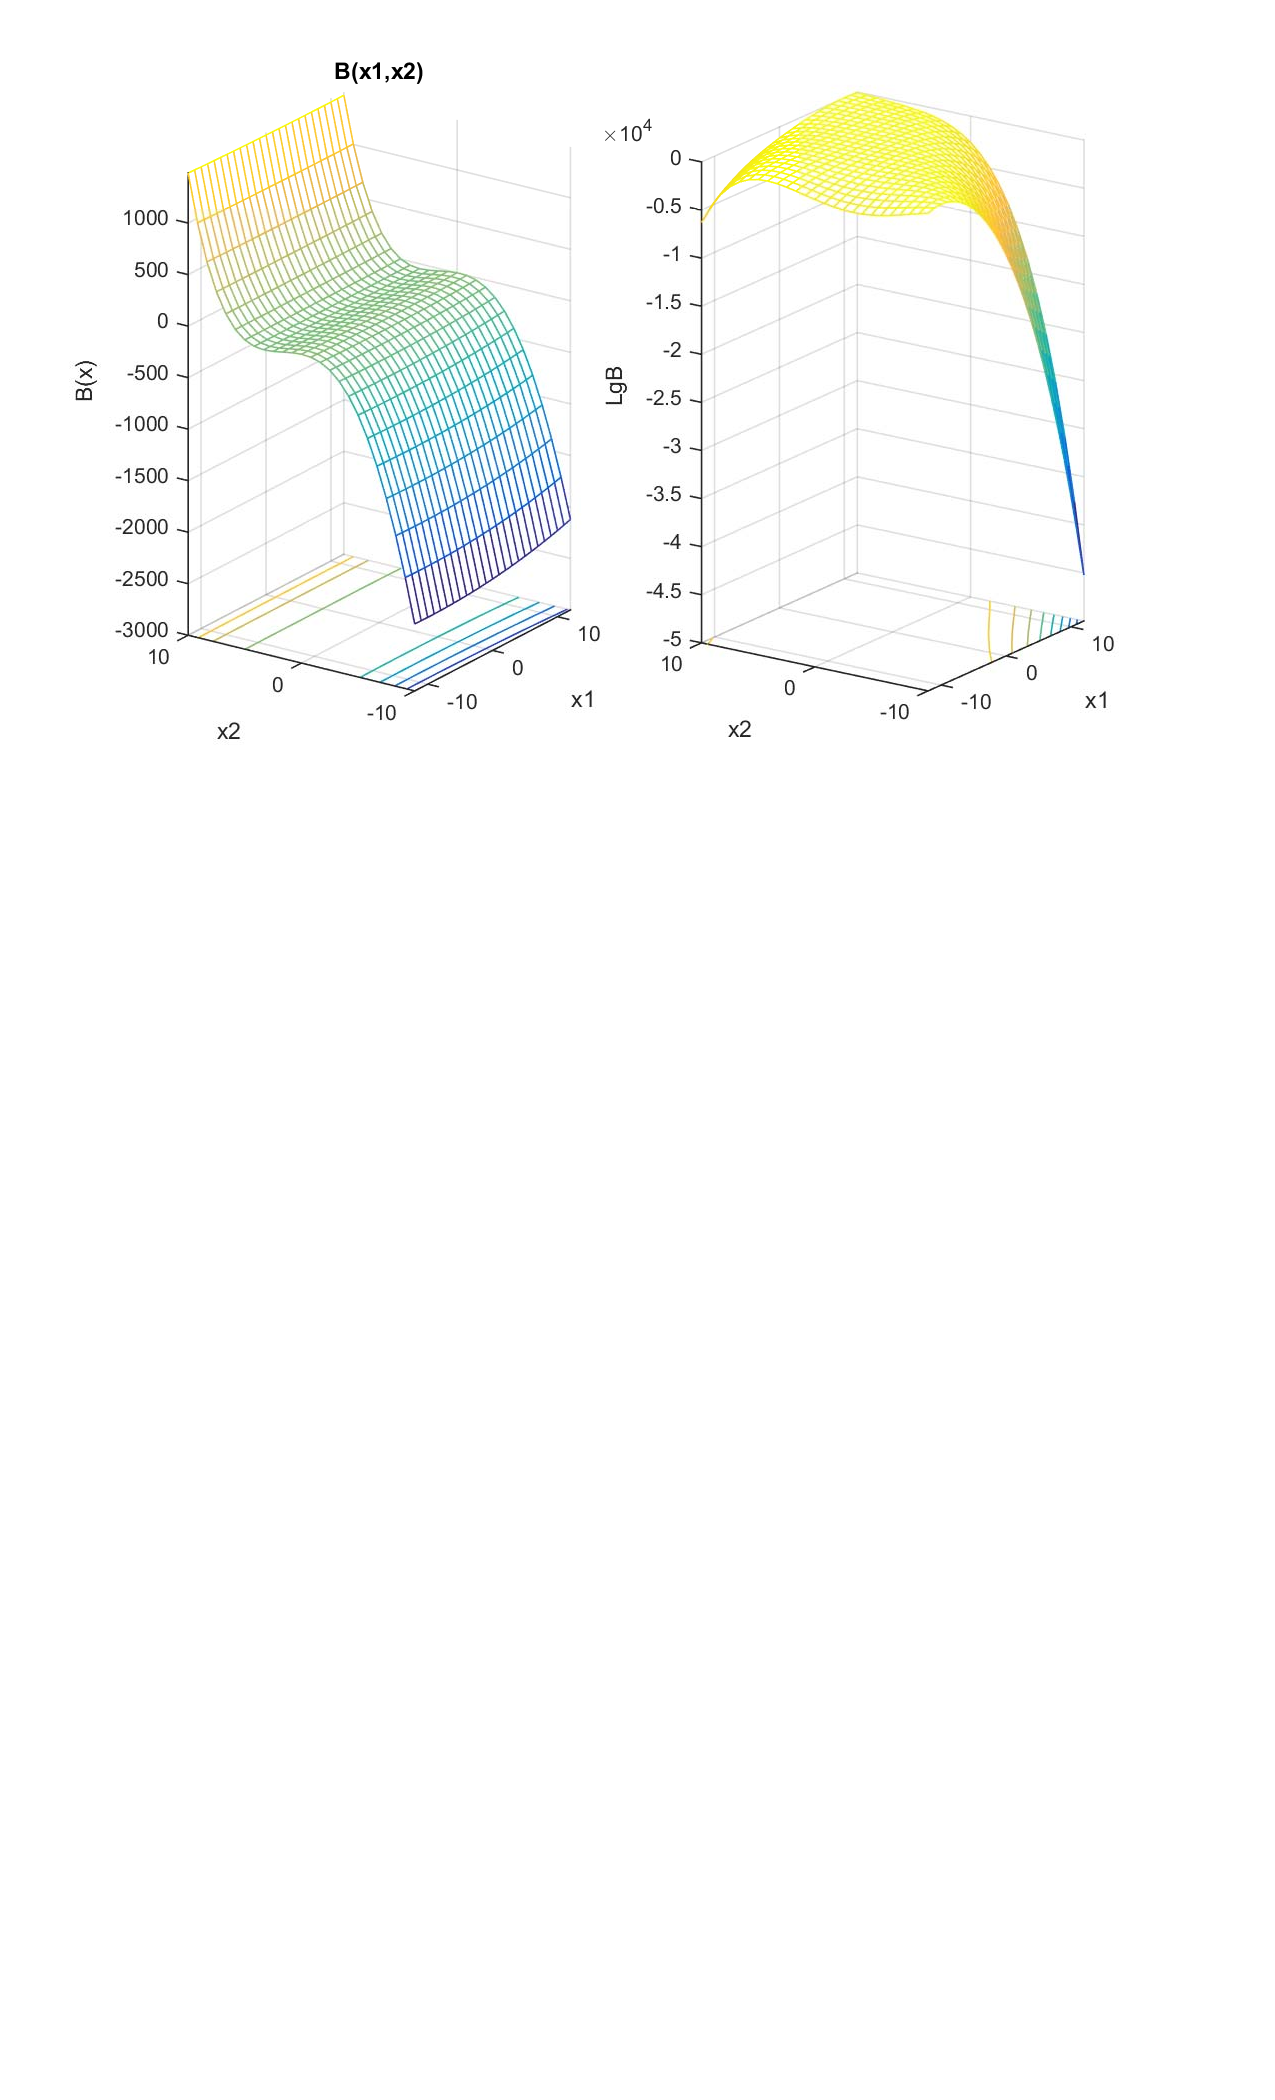
\includegraphics[width=0.7\textwidth]{Bxtilde5.pdf}
\caption{(\Autoref{case3}) $B(x_1,x_{ref})$ of degree 0:4, all other monomials of degree 0:2. \texttt{feasratio=1}, \texttt{numerr=1}, \texttt{res.norm=1e-7}, leading term coefficient 9e-5.}
\label{fig:Bxtilde5}
\end{figure}

\begin{figure}[h]
\centering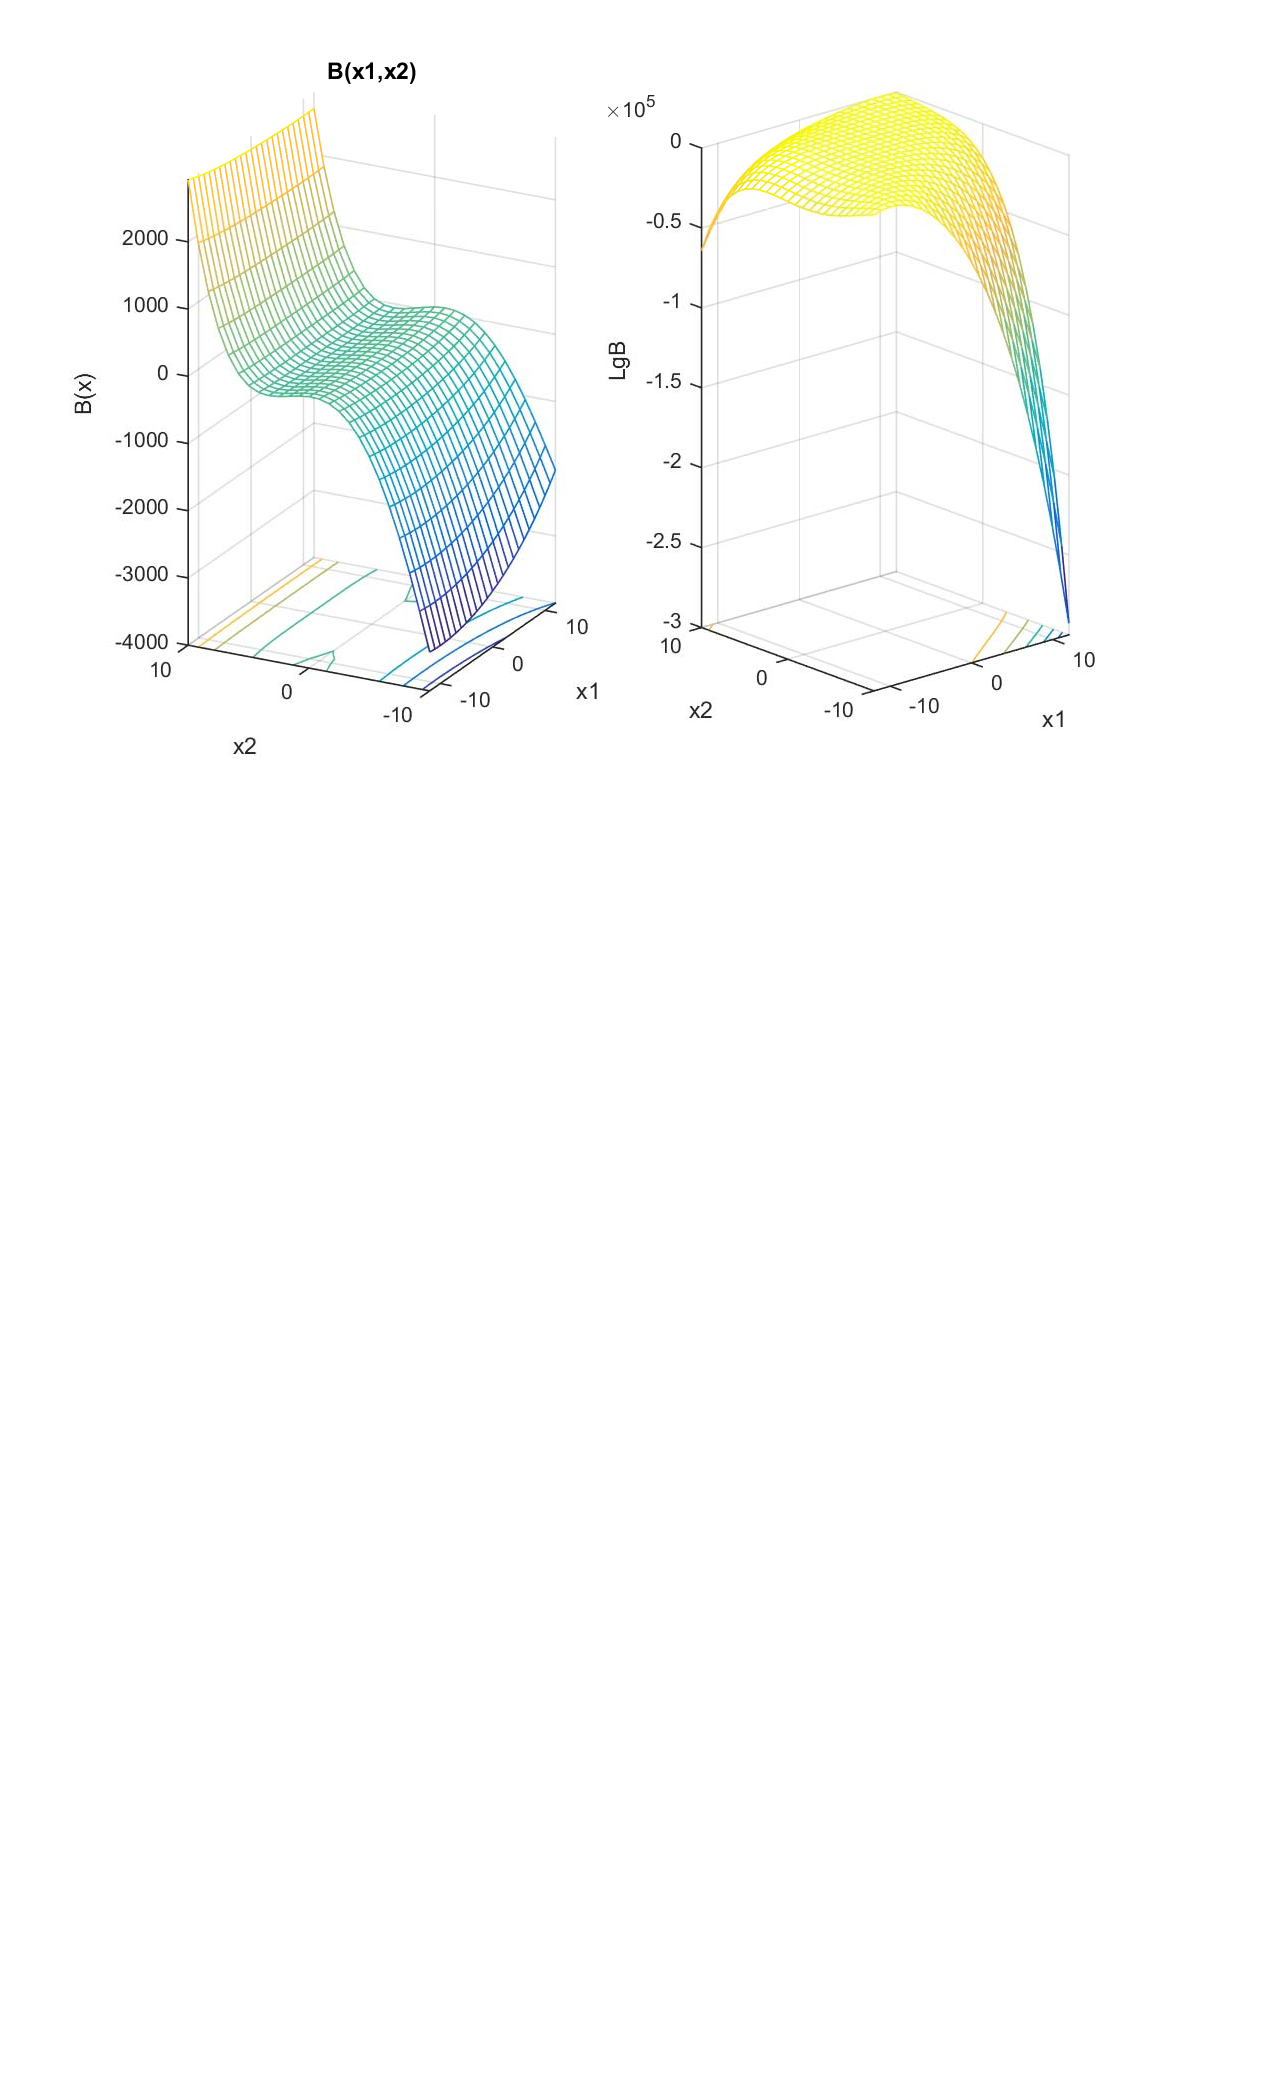
\includegraphics[width=0.7\textwidth]{Bxtilde6.pdf}
\caption{(\Autoref{case3}) $B(x_1,x_{ref})$ of degree 0:4, all other monomials of degree 0:4. \texttt{feasratio=1}, \texttt{numerr=1}, \texttt{res.norm=3e-6}, leading term coefficient 1e-3.}
\label{fig:Bxtilde6}
\end{figure}

\begin{figure}[h]
\centering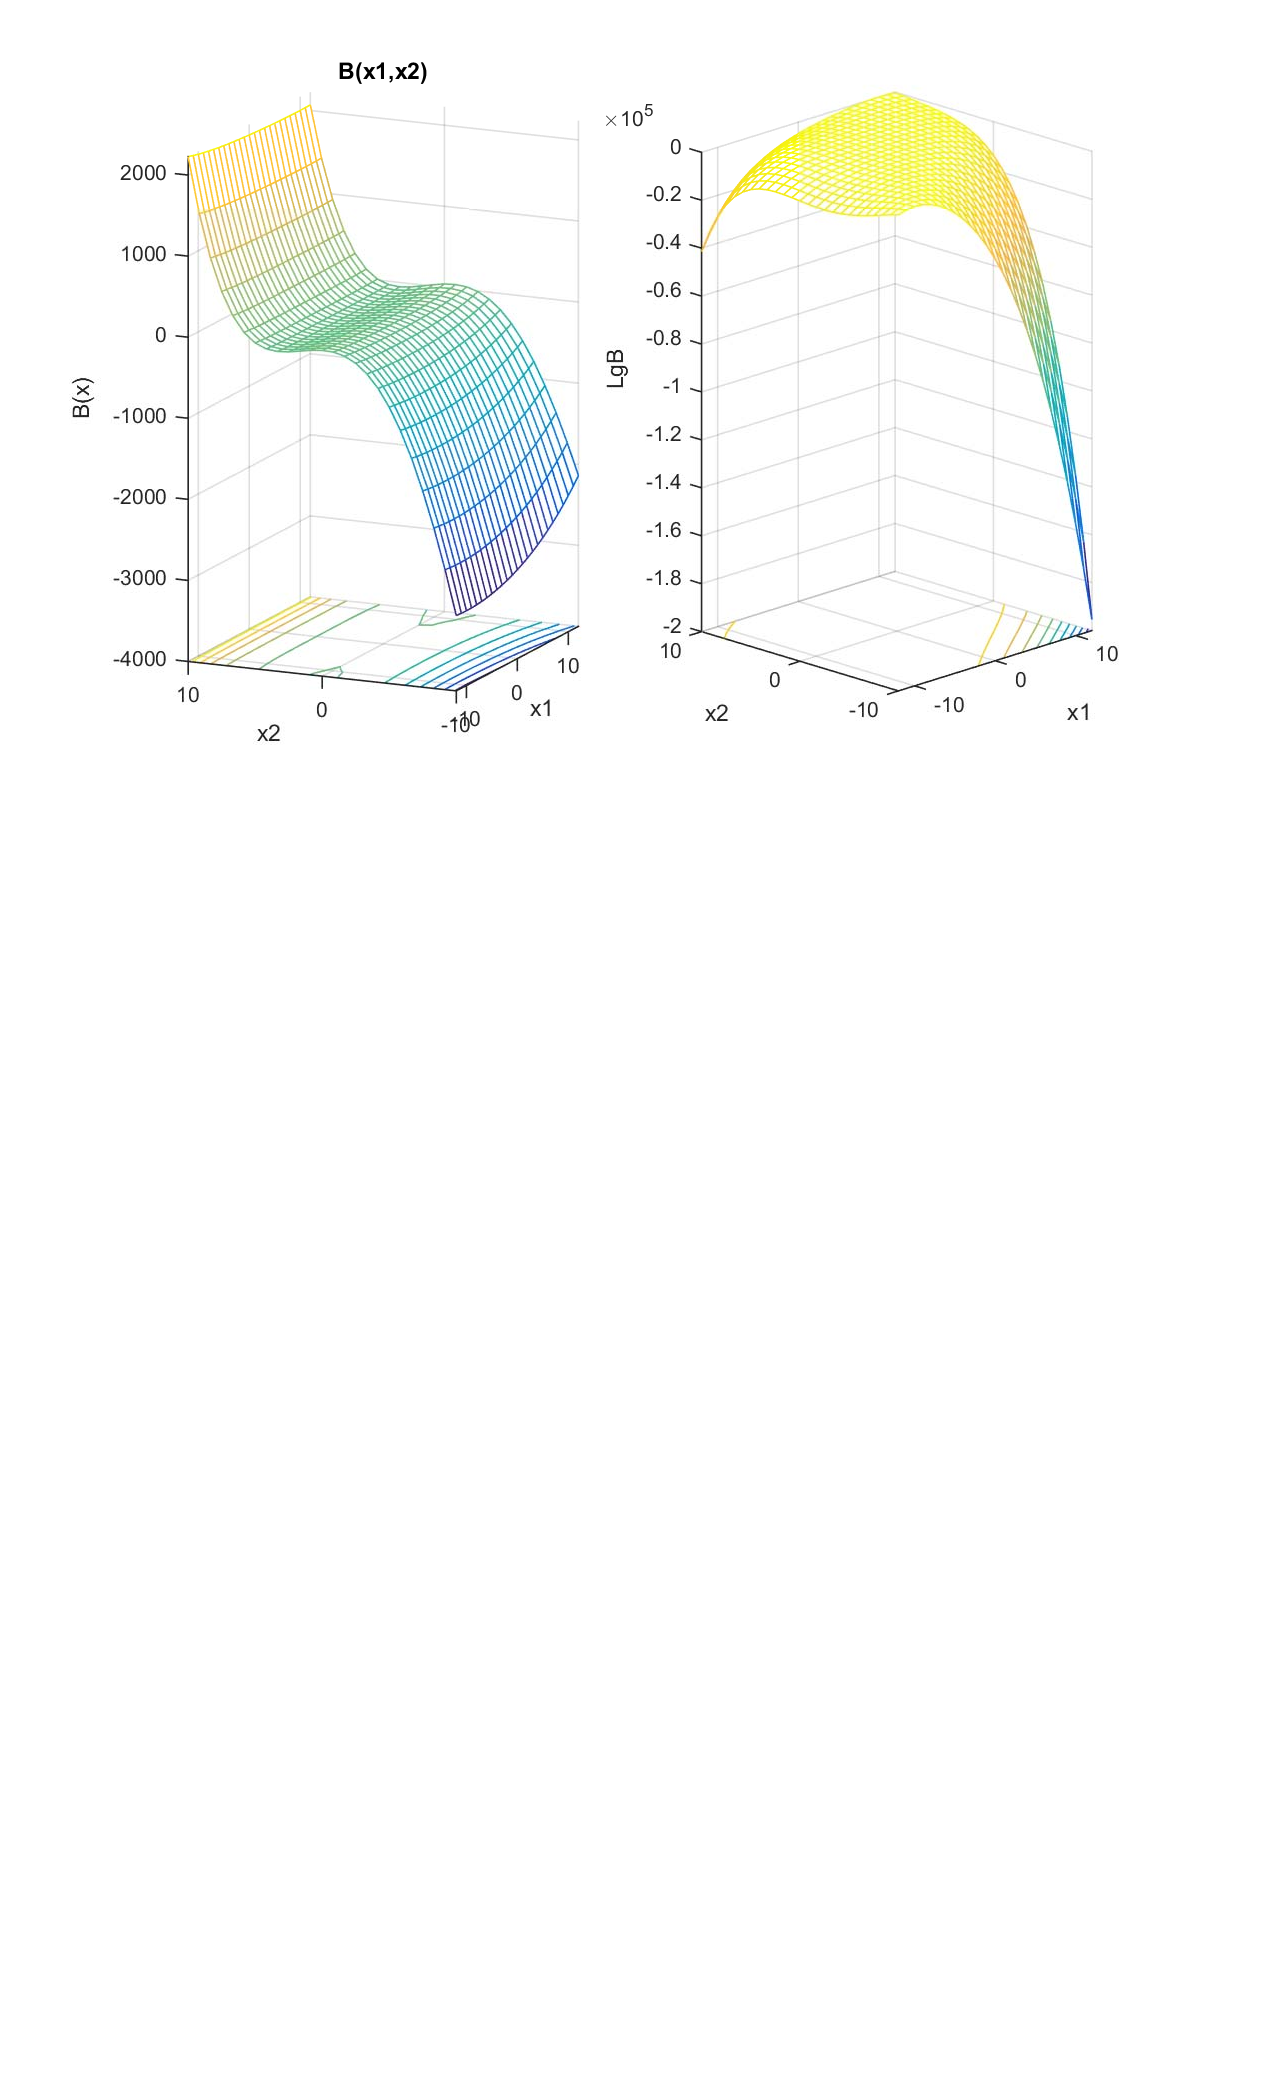
\includegraphics[width=0.7\textwidth]{Bxtilde7.pdf}
\caption{(\Autoref{case3}) $B(x_1,x_{ref})$ of degree 0:4,  monomials [used for $q$s multiplied with $g(x_1)$s] of degree 0:4 while monomials [used for $q$s multiplied with $g(x_{ref})$s] are of degree 0:2, to try to "weight" the $g(x_1)$ functions higher. \texttt{feasratio=1}, \texttt{numerr=1}, \texttt{res.norm=1e-6}, leading term coefficient 8e-4.}
\label{fig:Bxtilde7}
\end{figure}

\begin{figure}[H]
\centering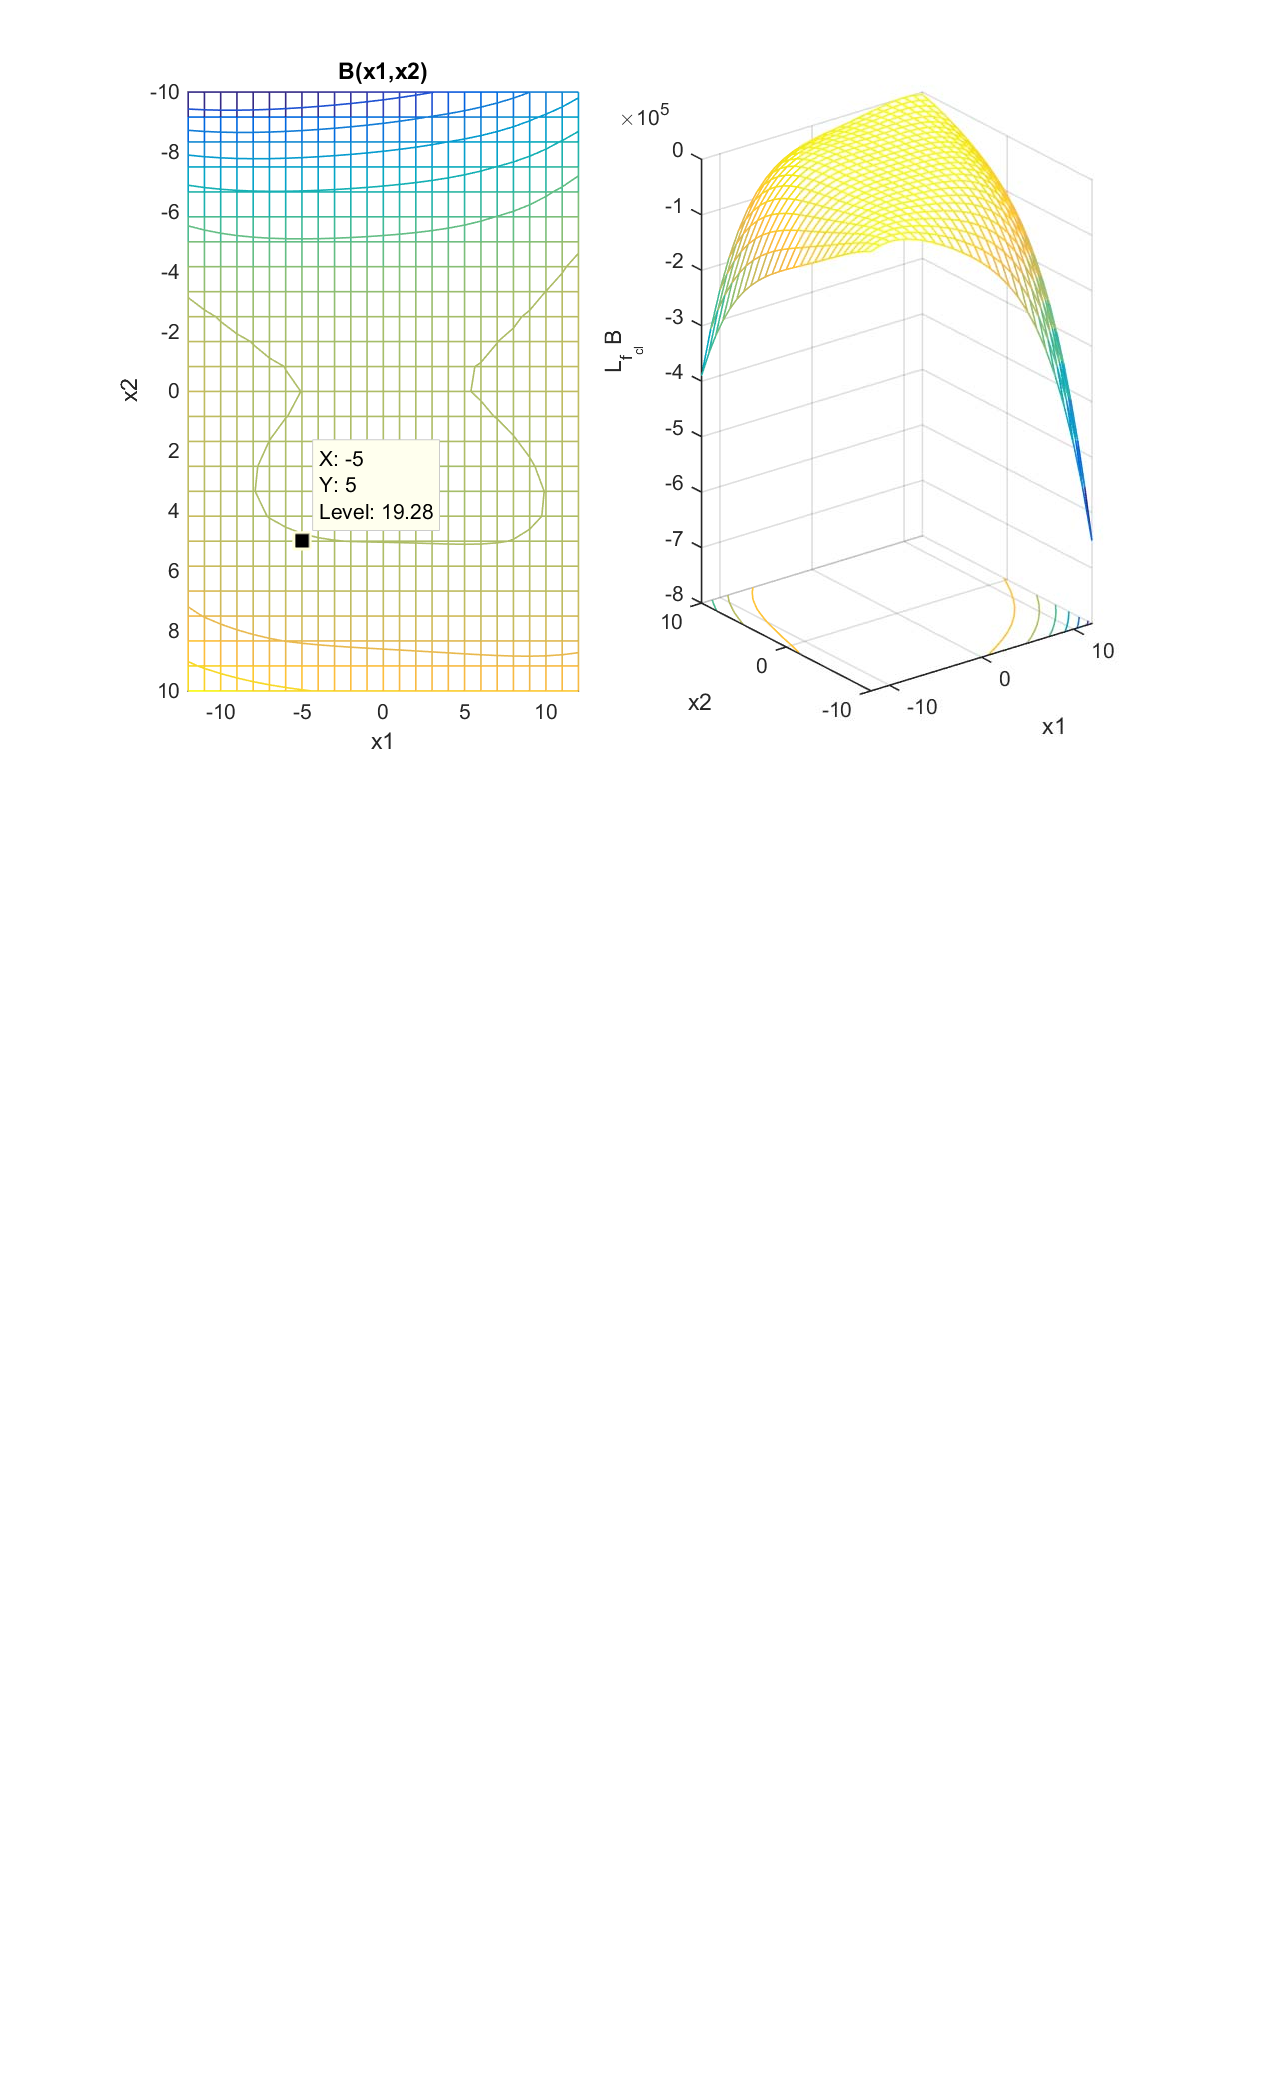
\includegraphics[width=0.7\textwidth]{Bxtilde9.pdf}
\caption{(\Autoref{case3}) Same as in \autoref{fig:Btilde7}, now increased monomial degrees [used for $q$s multiplied with $g(x_1)$s] to 0:5. \texttt{feasratio=1}, \texttt{numerr=1}, \texttt{res.norm=5e-6}, leading term coefficient 1e-2.}
\label{fig:Bxtilde9}
\end{figure}

\begin{figure}[H]
\centering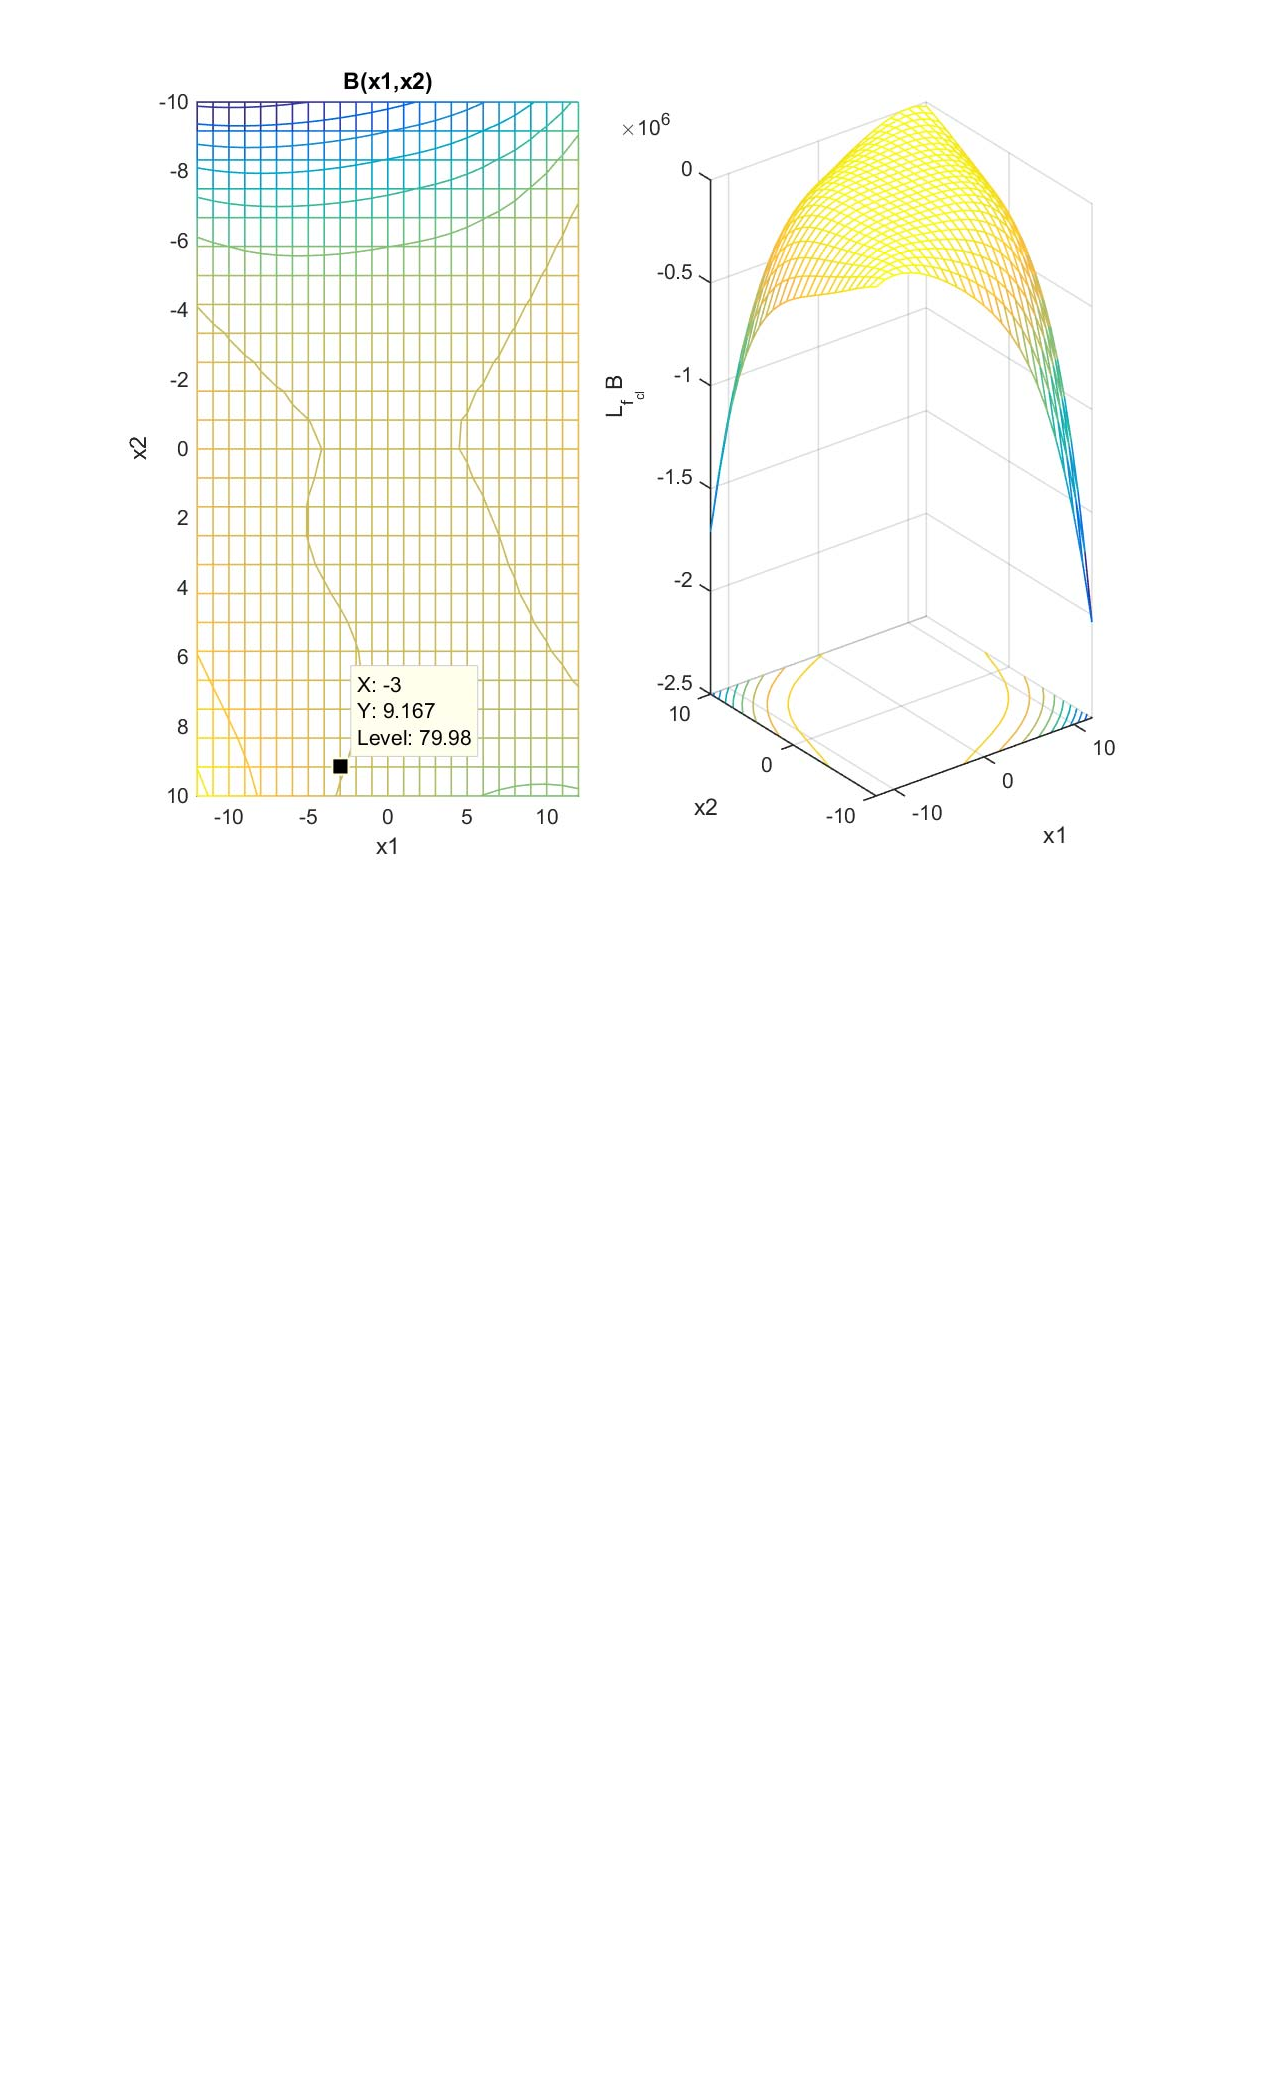
\includegraphics[width=0.7\textwidth]{Bxtilde10.pdf}
	\caption{(\Autoref{case3}) Same as in \autoref{fig:Bxtilde9}, now increased monomial degrees [used for $q$s multiplied with $g(x_1)$s] to 0:6. \texttt{feasratio=1}, \texttt{numerr=1}, \texttt{res.norm=3e-6}, leading term coefficient 4e-2.}
	\label{fig:Bxtilde10}
\end{figure}

\begin{figure}[H]
	\centering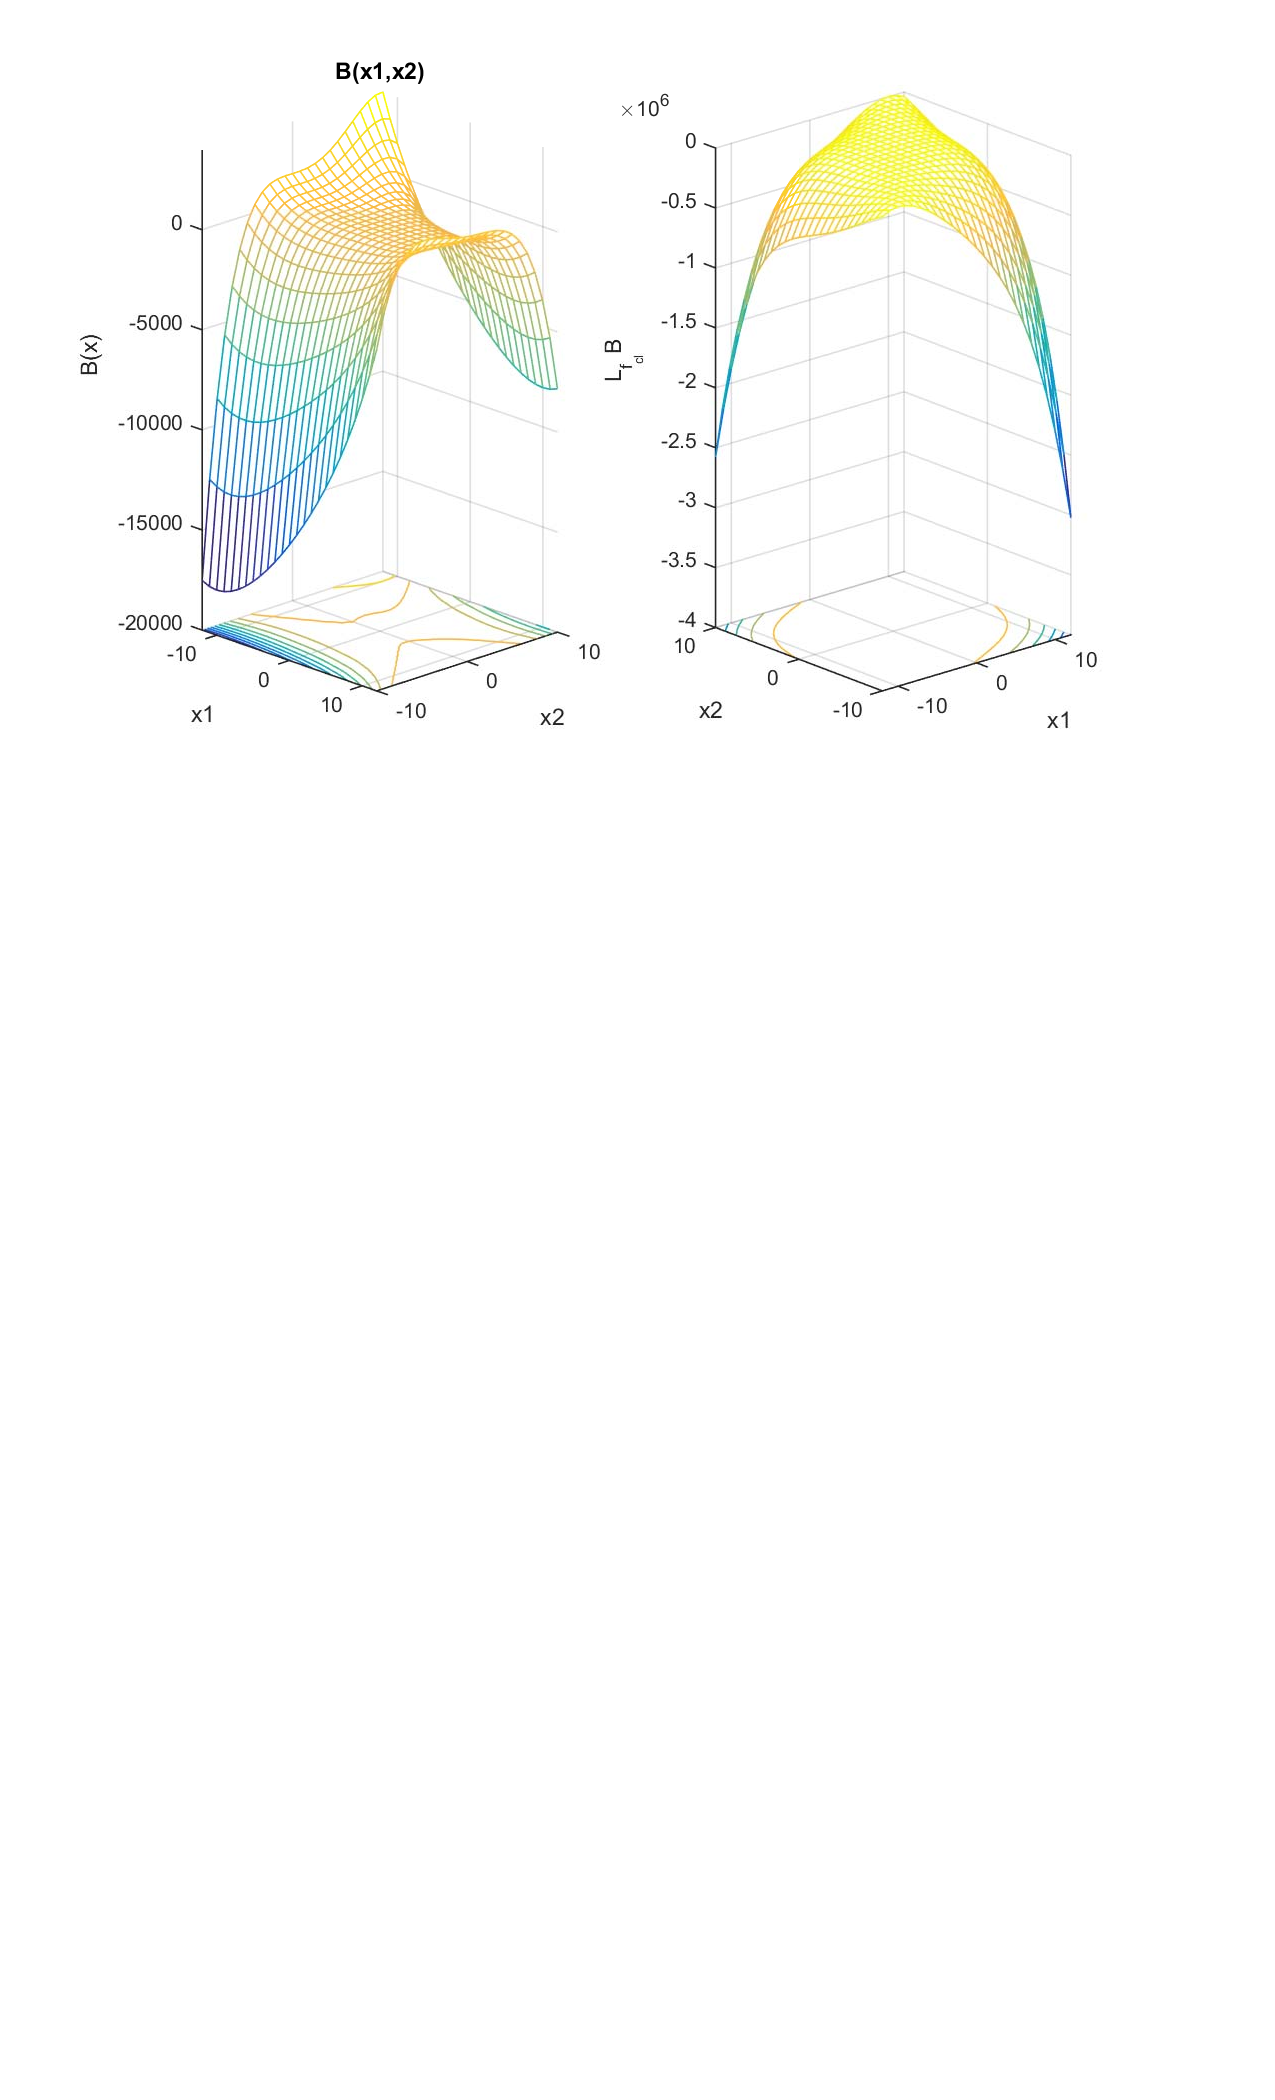
\includegraphics[width=0.7\textwidth]{Bxtilde11.pdf}
	\caption{(\Autoref{case3}) Same as in \autoref{fig:Bxtilde10}, now with all monomial degrees 0:6. \texttt{feasratio=0.9989}, \texttt{numerr=1}, \texttt{res.norm=1e-5}, leading term coefficient 6e-2.}
	\label{fig:Bxtilde11}
\end{figure}

\begin{figure}[H]
	\centering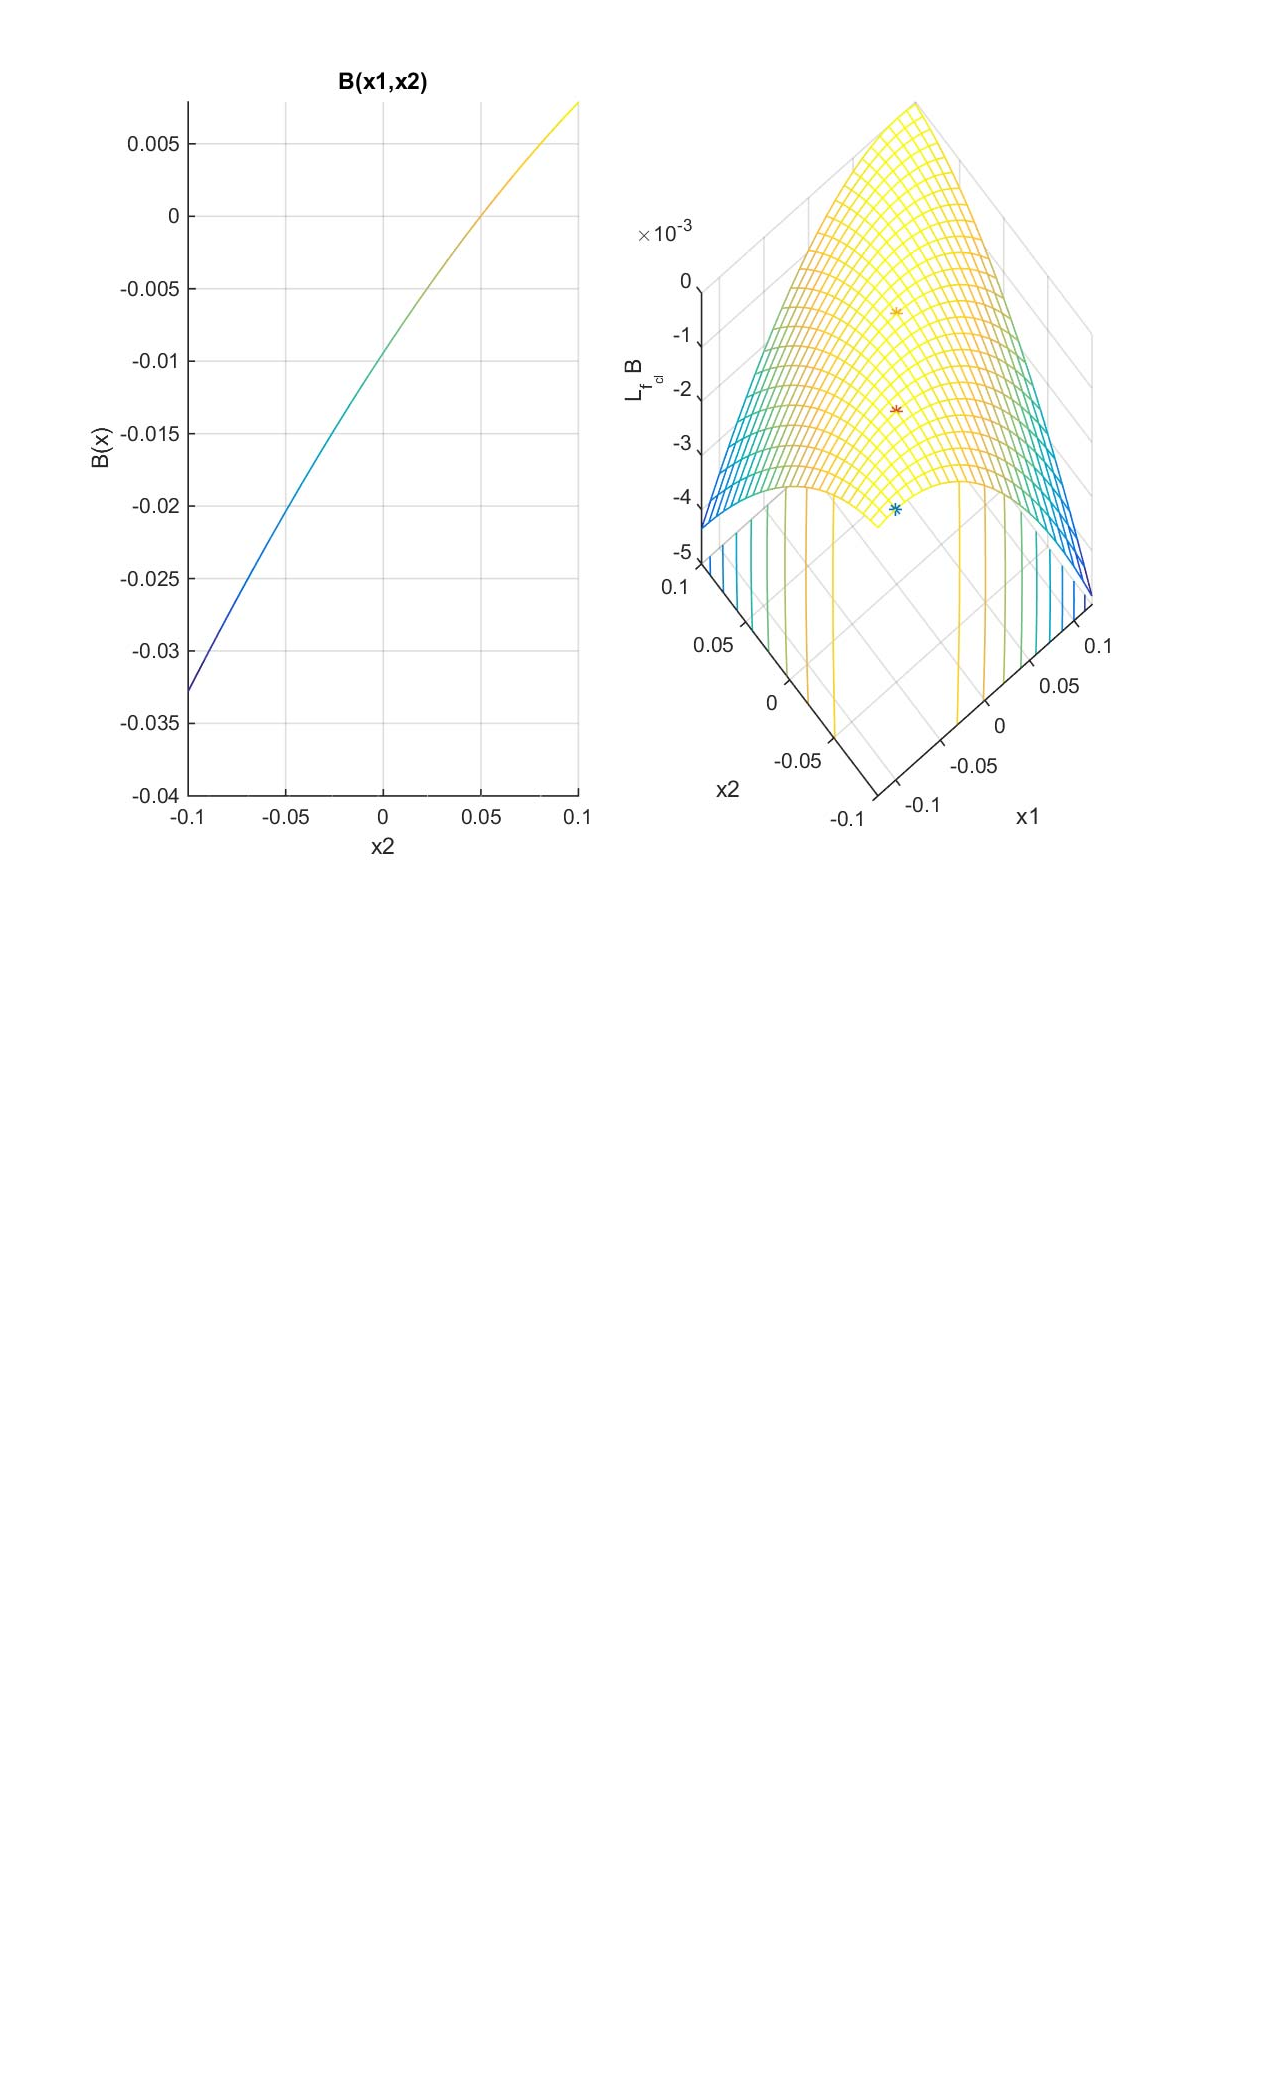
\includegraphics[width=0.7\textwidth]{Bxtilde12.pdf}
	\caption{(\Autoref{case3}) Same as in \autoref{fig:Bxtilde11}, changed unit back from [cm] to [m] i.e. changed scaling to 1. \texttt{feasratio=1}, \texttt{numerr=0} \textcolor{red}{notice!}, \texttt{res.norm=1e-9}, leading term coefficient 5e-4. Looks like ONLY a function of $x_{ref}$ \textcolor{red}{why??}}
	\label{fig:Bxtilde12}
\end{figure}

\begin{figure}[H]
	\centering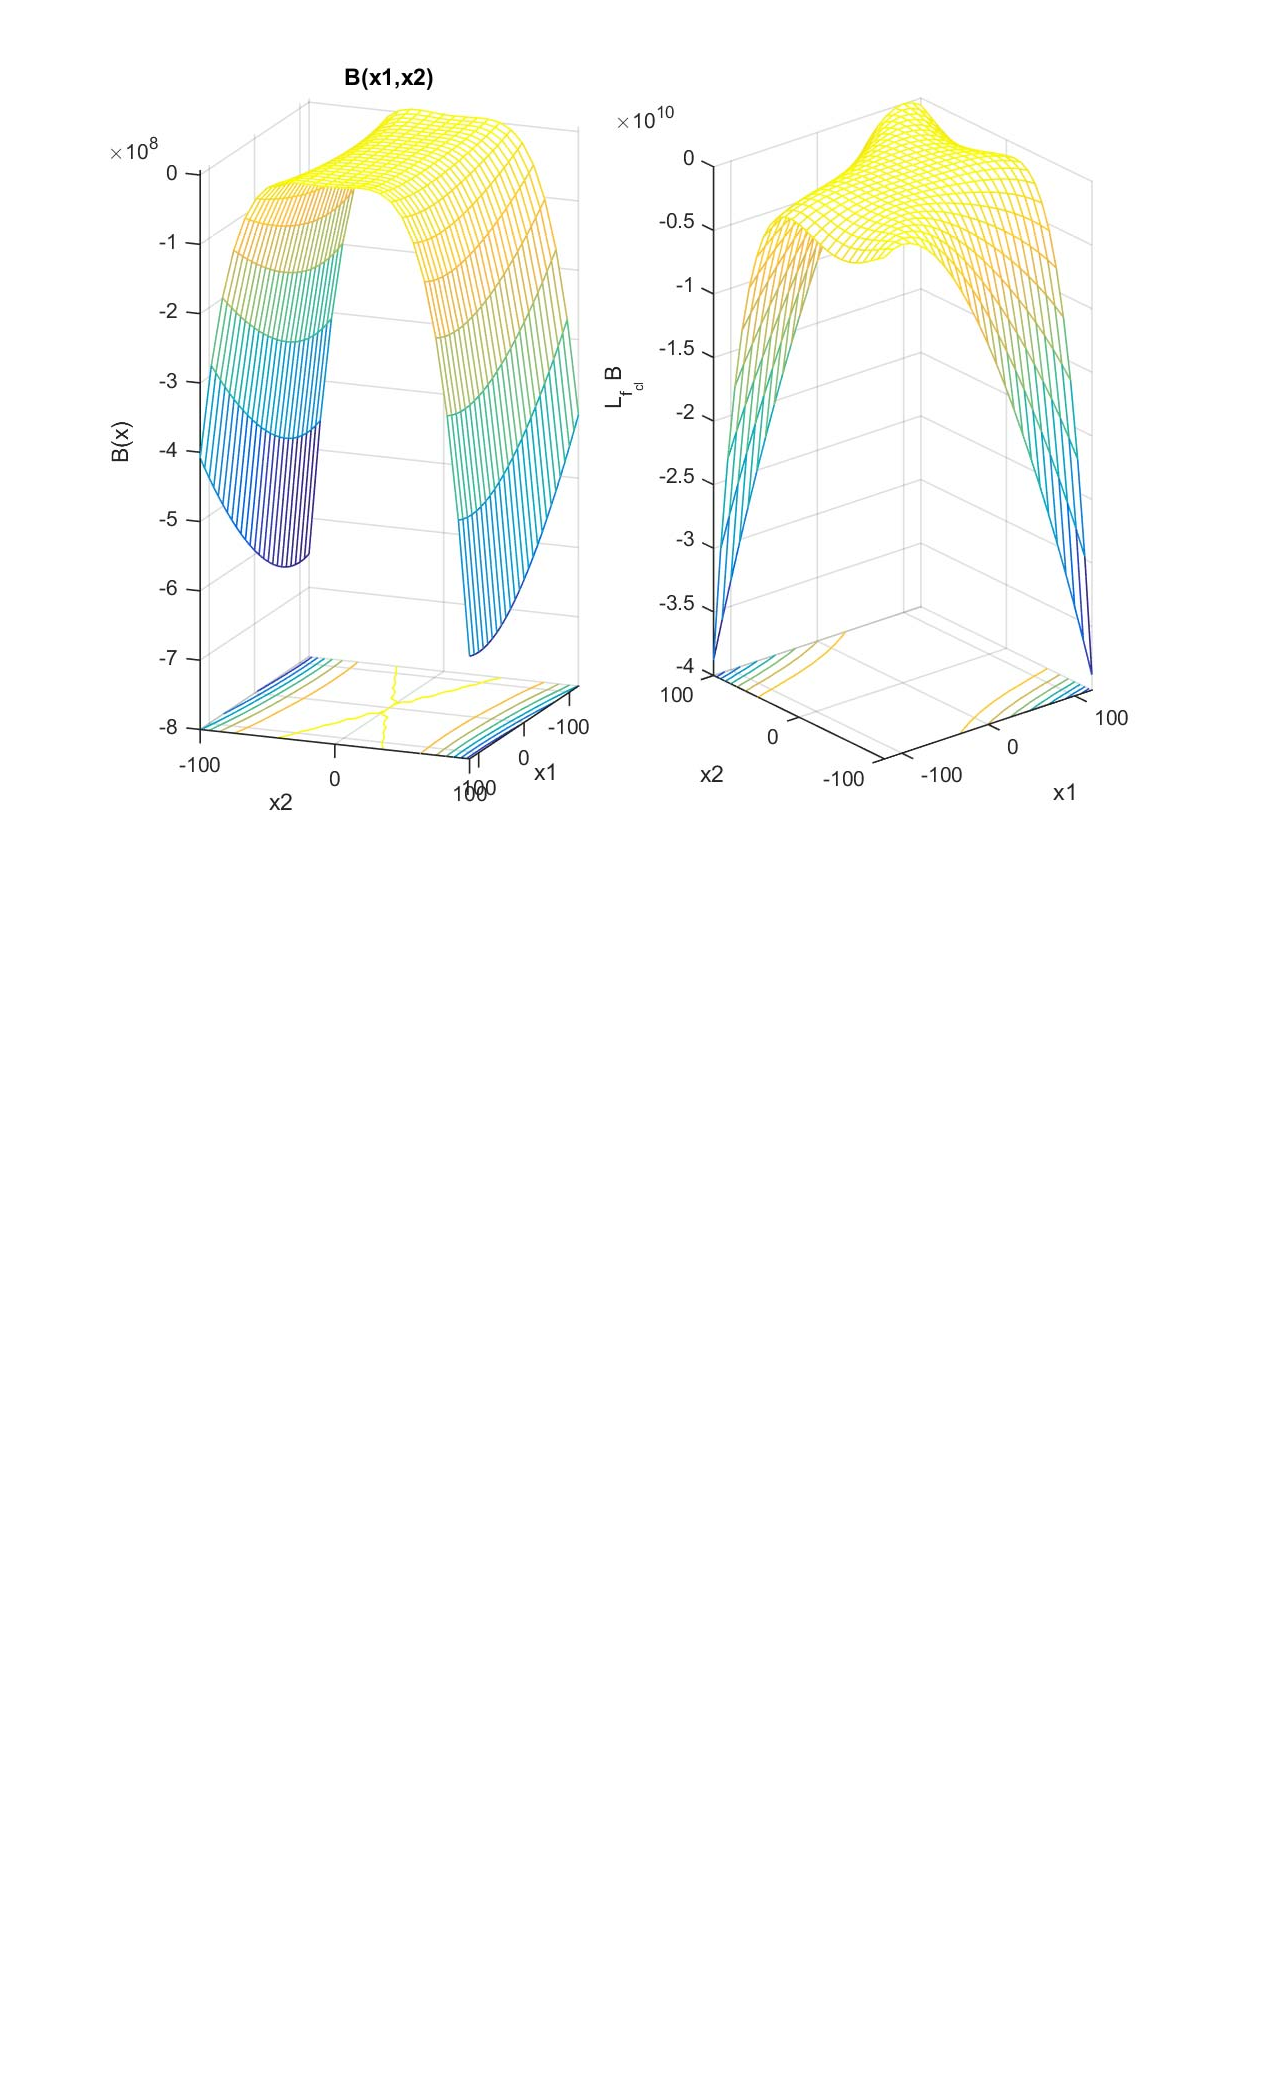
\includegraphics[width=0.7\textwidth]{Bxtilde13.pdf}
	\caption{(\Autoref{case3}) Same as in \autoref{fig:Bxtilde11}, changed unit  to [mm] i.e. changed scaling to 1000. \texttt{feasratio=1.0001}, \texttt{numerr=1}, \texttt{res.norm=4e-6}, leading term coefficient 1e-2.}
	\label{fig:Bxtilde13}
\end{figure}





\newpage
\subsection{Case 4}\label{case4}
\begin{figure}[htbp]
\centering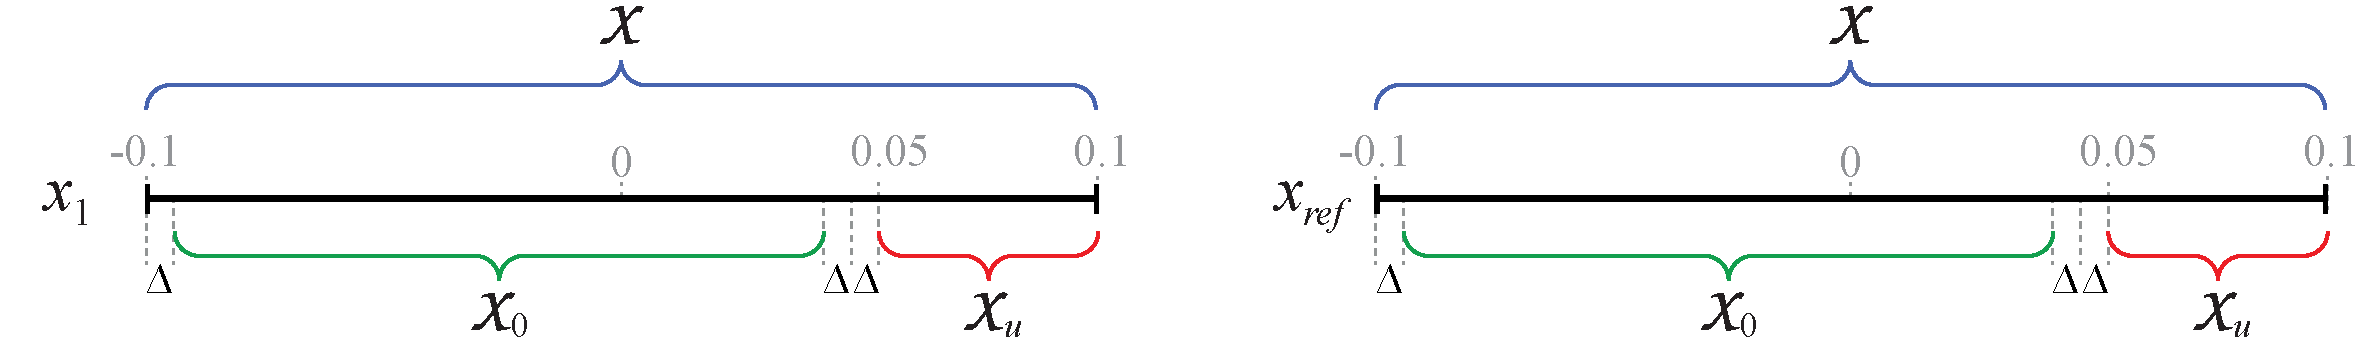
\includegraphics[width=\textwidth]{intervals_for_sos4.pdf}
\caption{All three sets are defined by both $x_1$ and $x_{ref}$, both defined in the same intervals. Now $\mathcal{X}_0$ is slightly smaller than in the previous cases.}
\label{fig:intervals_for_sos4}
\end{figure}
\begin{subequations}\label{eq:sets_case4}
With sets defined as in \autoref{fig:intervals_for_sos1}:
\begin{align}
\mathcal{X} &= \begin{bmatrix} -0.1 & 0.1\end{bmatrix} \times \begin{bmatrix} -0.1 & 0.1\end{bmatrix}\\
\mathcal{X}_u &= \begin{bmatrix} 0.05 & 0.1\end{bmatrix} \times \begin{bmatrix} 0.05 & 0.1\end{bmatrix}\\
\mathcal{X}_0 &=\begin{bmatrix} -0.1+\Delta & 0.05-2\Delta\end{bmatrix} \times \begin{bmatrix} -0.1+\Delta & 0.05-2\Delta\end{bmatrix}
\end{align}
\end{subequations}

\begin{figure}[h]
\centering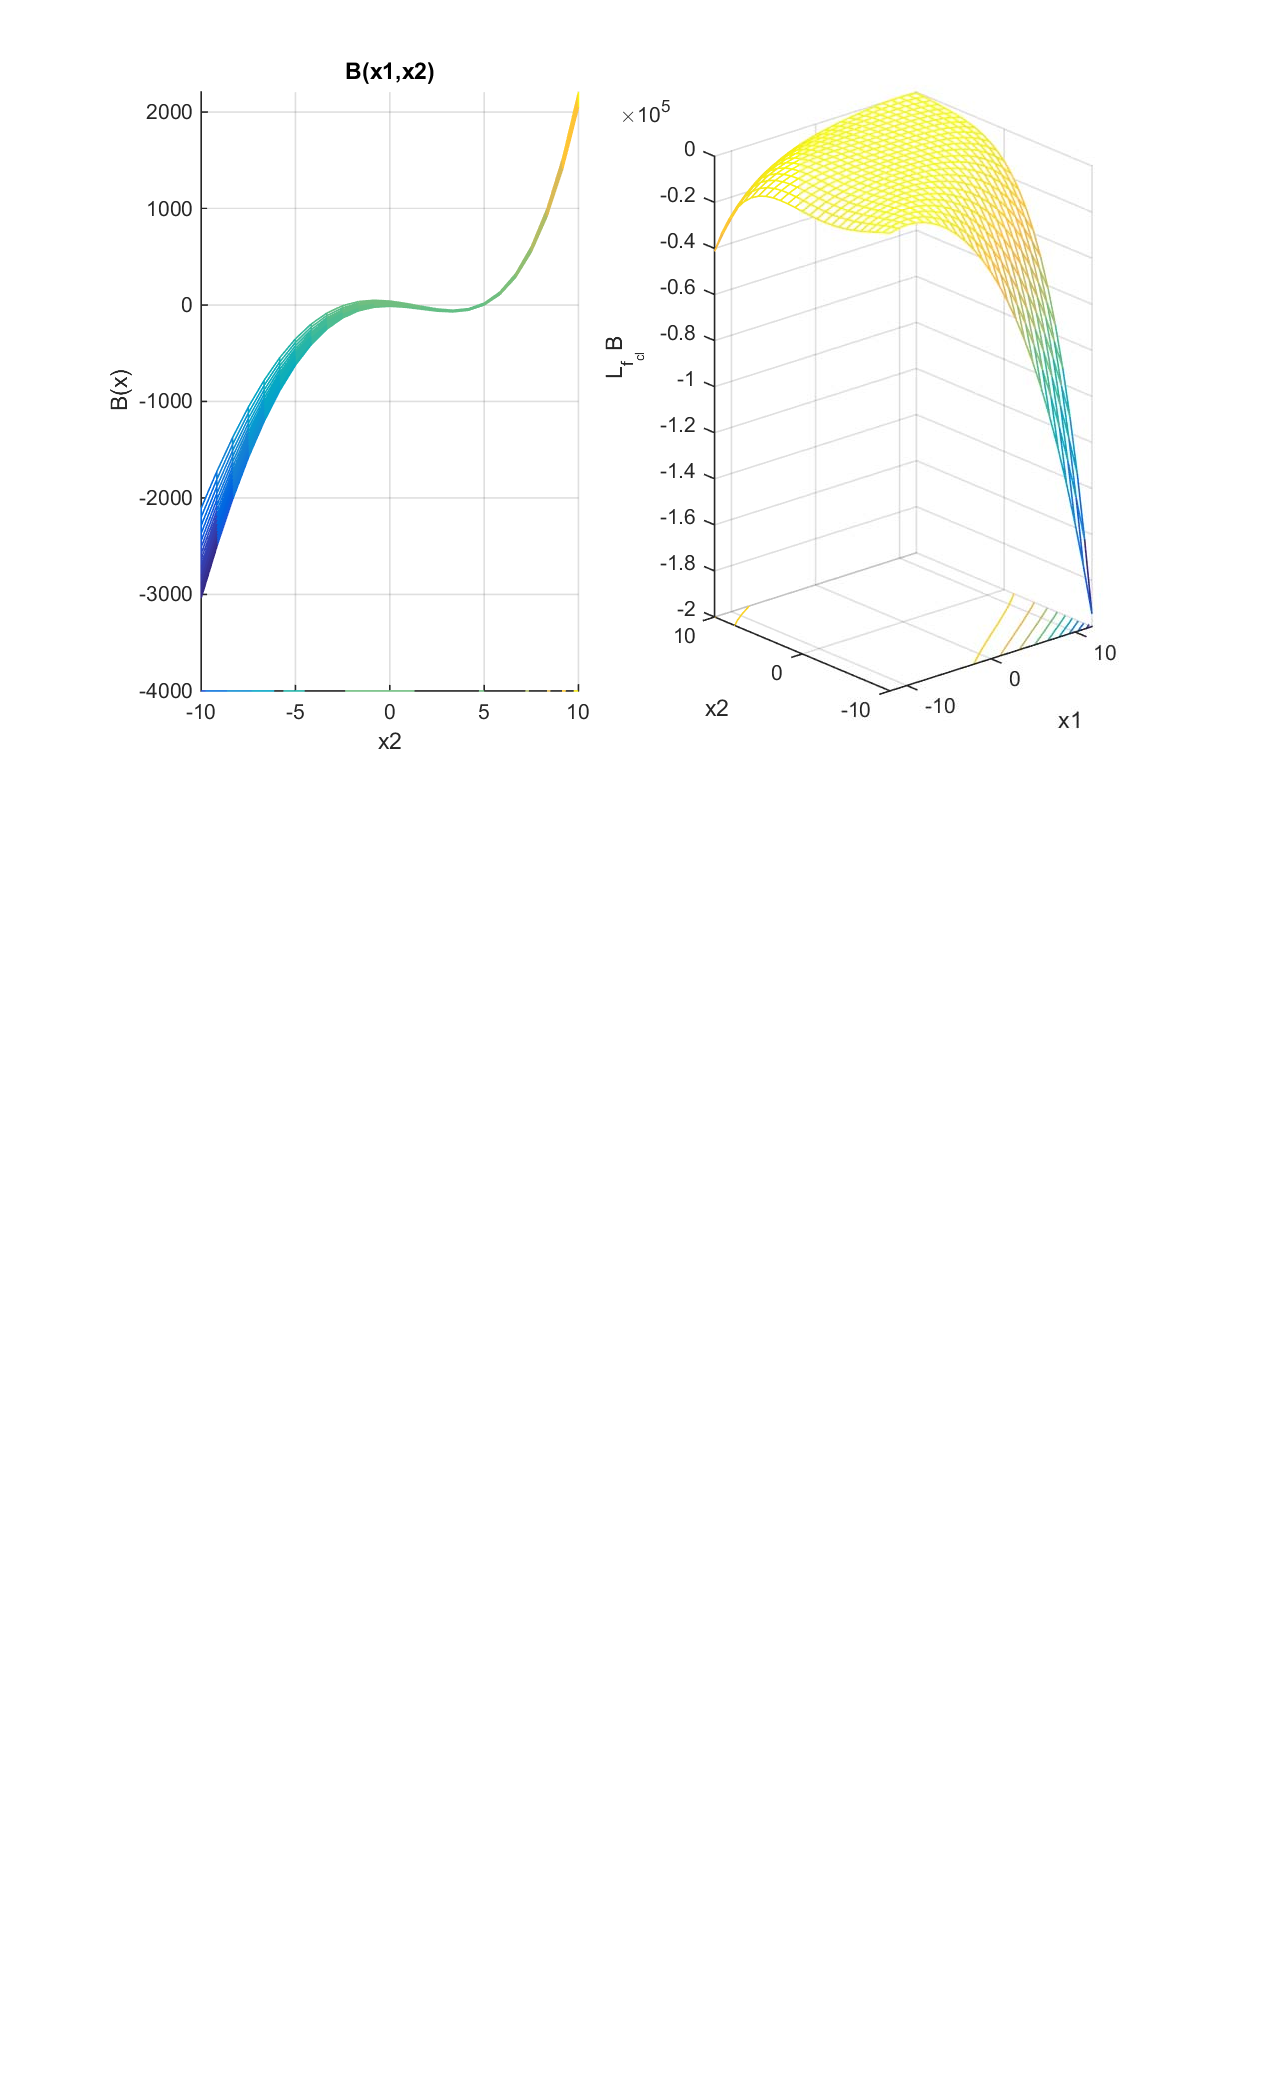
\includegraphics[width=0.7\textwidth]{Bxtilde8.pdf}
\caption{(\Autoref{case4}) $B(x_1,x_{ref})$ of degree 0:4,  monomials [used for $q$s multiplied with $g(x_1)$s] of degree 0:4 while monomials [used for $q$s multiplied with $g(x_{ref})$s] are of degree 0:2, to try to "weight" the $g(x_1)$ functions higher. \texttt{feasratio=1}, \texttt{numerr=1}, \texttt{res.norm=1e-6}, leading term coefficient 8e-4. \textcolor{red}{Exactly the same as without the $\Delta$-restriction on $\mathcal{X}_0$ with $x_1$.}}
\label{fig:Bxtilde8}
\end{figure}

\newpage
\section{Relaxed definition of the sets}
A new formulation of the sets is put forth, forming relaxed requirements for $B(x)$ compared to the set requirements for $B(x)$ given in Case 1 in \autoref{eq:sets_case1}, with $\mathcal{X}_u$ and $\mathcal{X}_0$ (corresponding to positivity and nonpositivity of $B(x)$, respectively) only required for the values of $x_{ref}$ that are in the set $\mathcal{X}$, and not for all values in $\mathbb{R}$.
\begin{figure}[htbp]
	\centering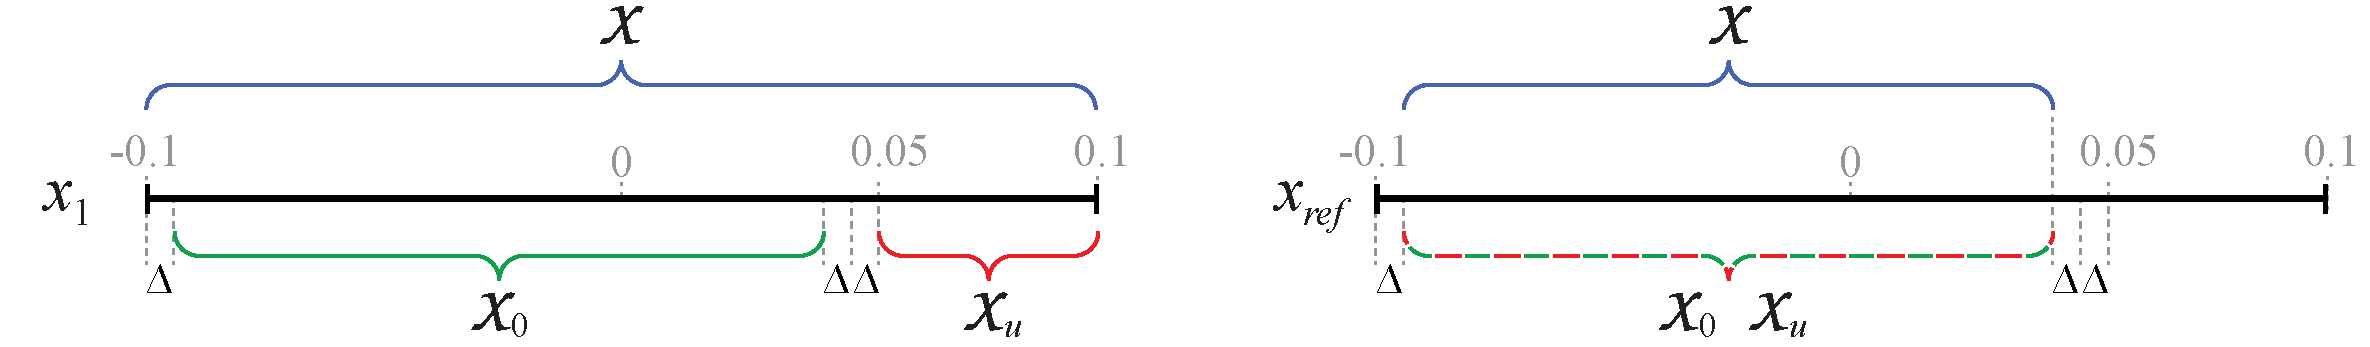
\includegraphics[width=\textwidth]{intervals_for_sos5.pdf}
	\caption{All three sets are defined by both $x_1$ and $x_{ref}$, with (un)safety defined by $x_1$, for the same interval of $x_{ref}$ in all three sets.}
	\label{fig:intervals_for_sos5}
\end{figure}

Note that as in case 4 in \autoref{eq:sets_case4} that the safe set is contracted by the value $\Delta$. \textcolor{red}{Test without this, and for larger values of $\Delta$.}
The sets are visualized in \autoref{fig:intervals_for_sos5} and formulated as:
\begin{subequations}\label{eq:sets_case5}
\begin{align}
	\mathcal{X} &= \begin{bmatrix} -0.1 & 0.1\end{bmatrix} \times \begin{bmatrix} -0.1+\Delta & 0.05-2\Delta\end{bmatrix}\\
	\mathcal{X}_u &= \begin{bmatrix} 0.05 & 0.1\end{bmatrix} \times \begin{bmatrix} -0.1+\Delta & 0.05-2\Delta\end{bmatrix}\\
	\mathcal{X}_0 &= \begin{bmatrix} -0.1+\Delta & 0.05-2\Delta\end{bmatrix} \times \begin{bmatrix} -0.1+\Delta & 0.05-2\Delta\end{bmatrix}
\end{align}
\end{subequations}
in code translating to
\begin{lstlisting}[language=matlab]
% Define space X in Rn
[a,b,c]=parabola(Xmin,Xmax); % get coefficients for parabola
gX1 = a*x1^2+b*x1+c;
...
[a,b,c]=parabola(Xmin+delta,Xumin-2*delta);
gX2 = a*xref^2+b*xref+c;
...
prog = sosineq(prog,-[diff(Bar,x1) diff(Bar,xref)]*fx-gX1*qX1-gX2*qX2);

% Define space Xu in X
[a,b,c]=parabola(Xumin,Xumax);
gXu1 = a*x1^2+b*x1+c;
...
[a,b,c]=parabola(Xmin+delta,Xumin-2*delta);
gXu2 = a*xref^2+b*xref+c;
...
prog = sosineq(prog,Bar-epsilon-gXu1*qXu1-gXu2*qXu2);

% Define space X0 in X
[a,b,c]=parabola(Xmin+delta,Xumin-2*delta);
gX01 = a*x1^2+b*x1+c;
...
[a,b,c]=parabola(Xmin+delta,Xumin-2*delta);
gX02 = a*xref^2+b*xref+c;

prog = sosineq(prog,-Bar-gX01*qX01-gX02*qX02);
\end{lstlisting}

\begin{figure}[H]
\vspace*{-5mm}
\subbottom[]{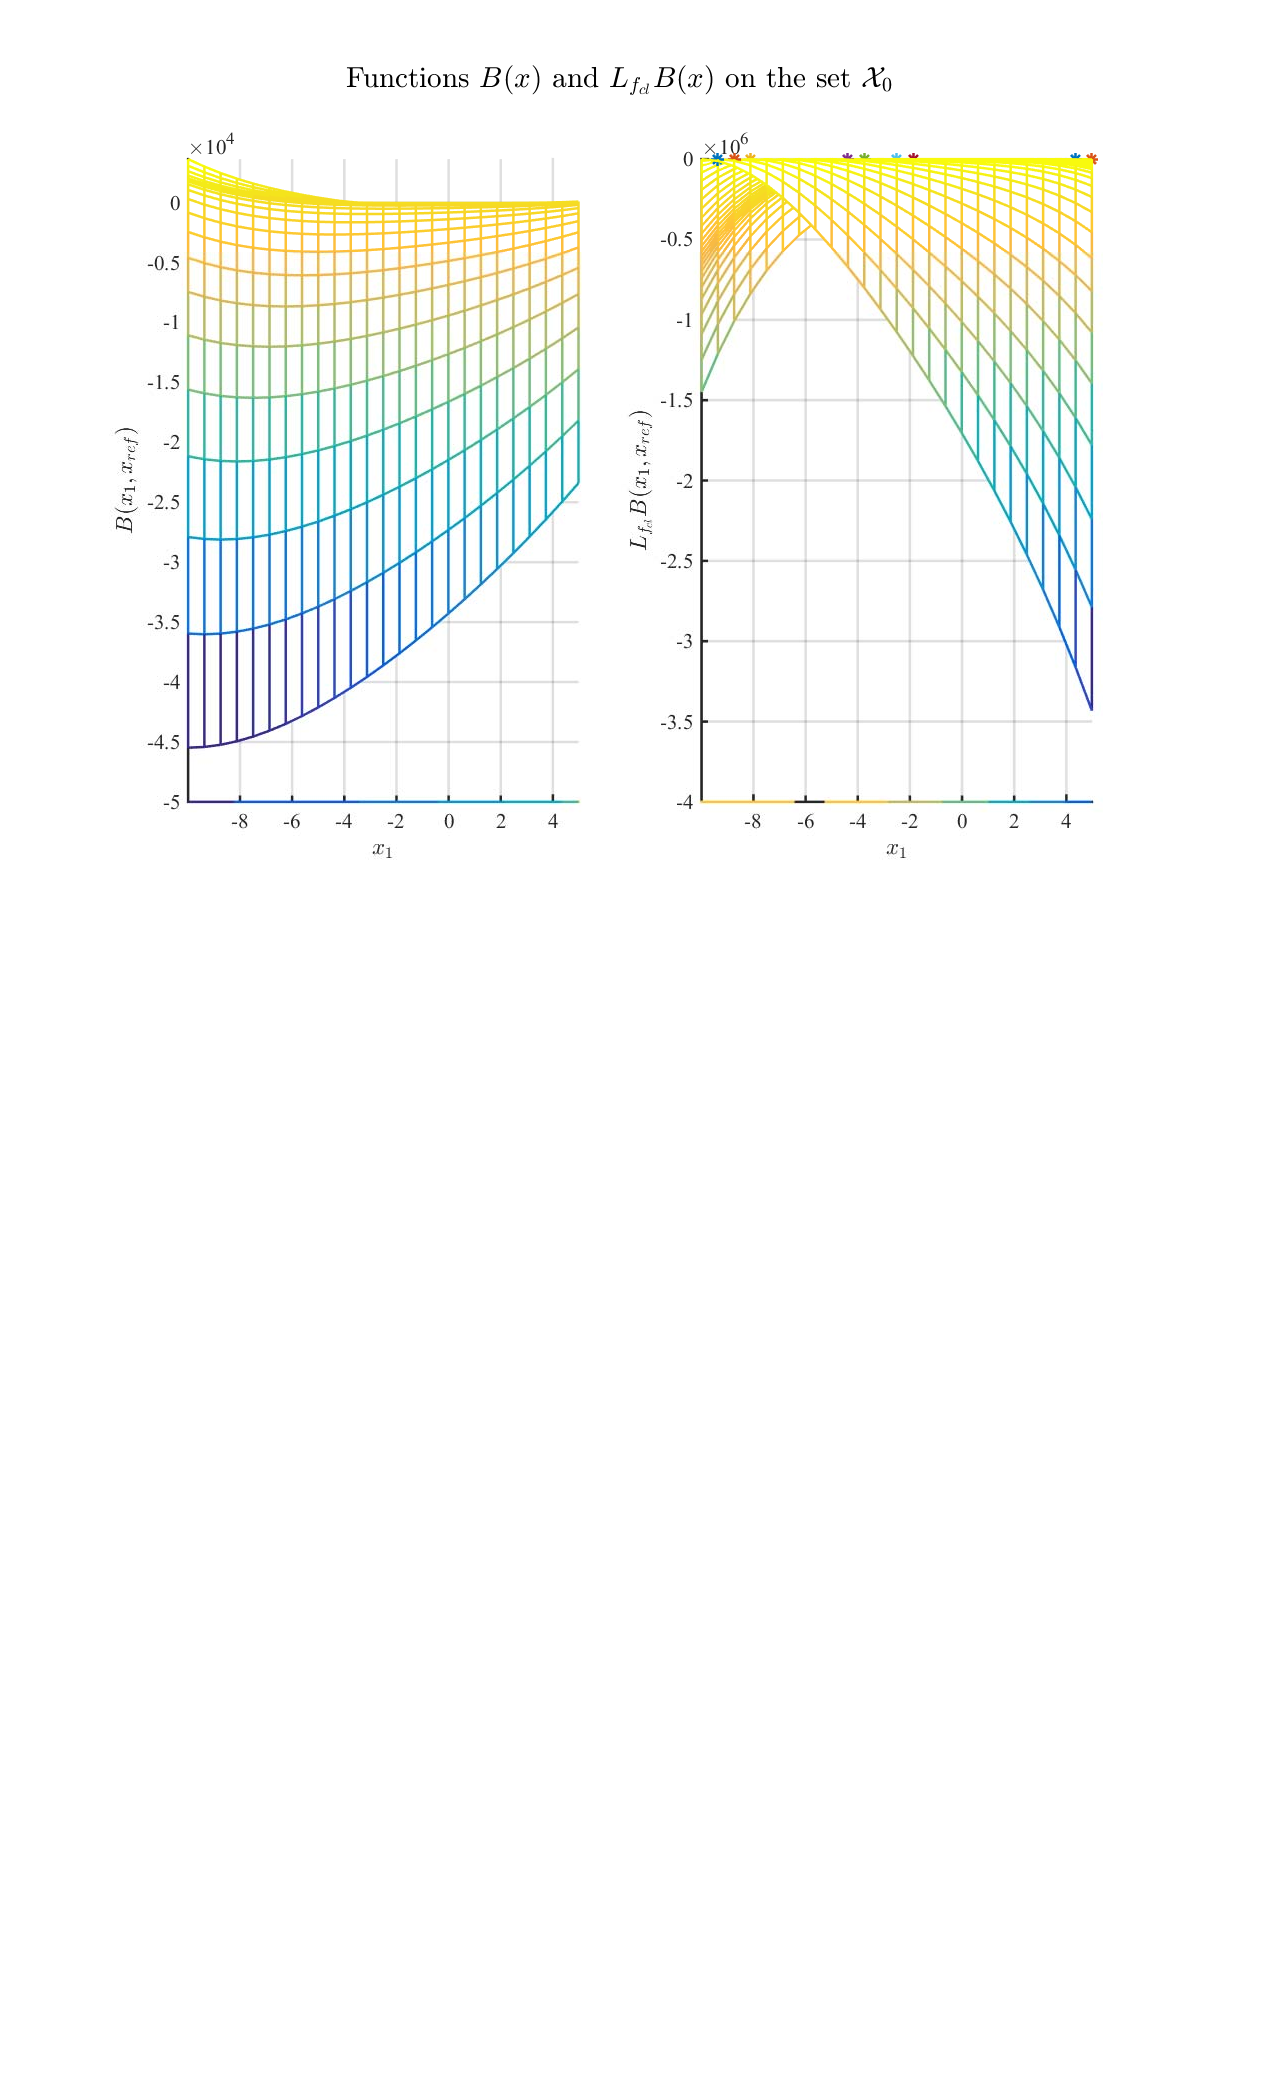
\includegraphics[width=0.5\textwidth]{Bnew1_X0_x1.pdf}}%
\subbottom[]{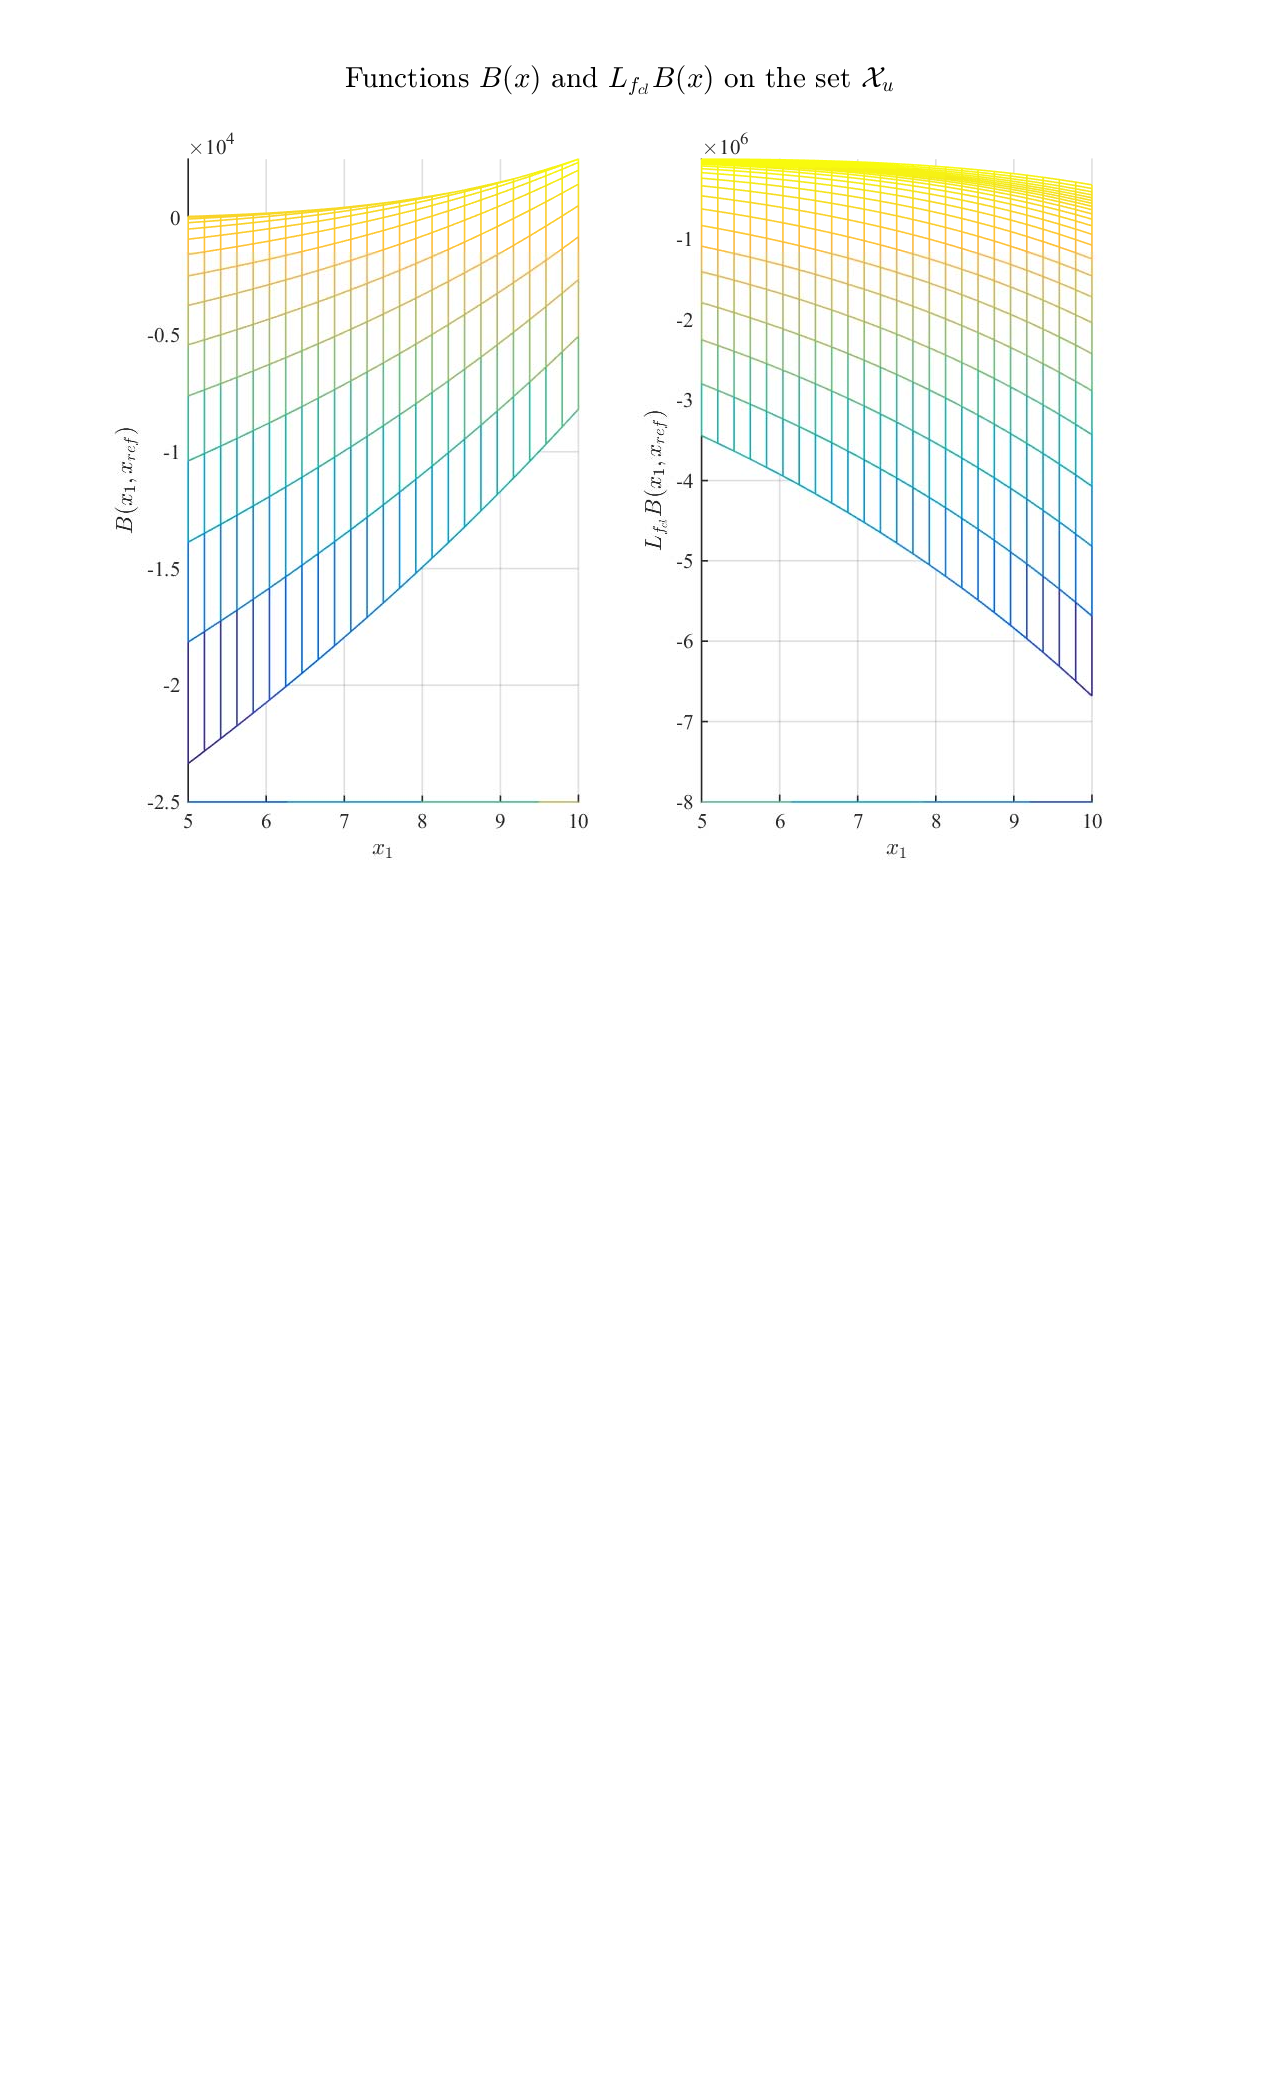
\includegraphics[width=0.5\textwidth]{Bnew1_Xu_x1.pdf}}%
\hspace{1mm}
\subbottom[]{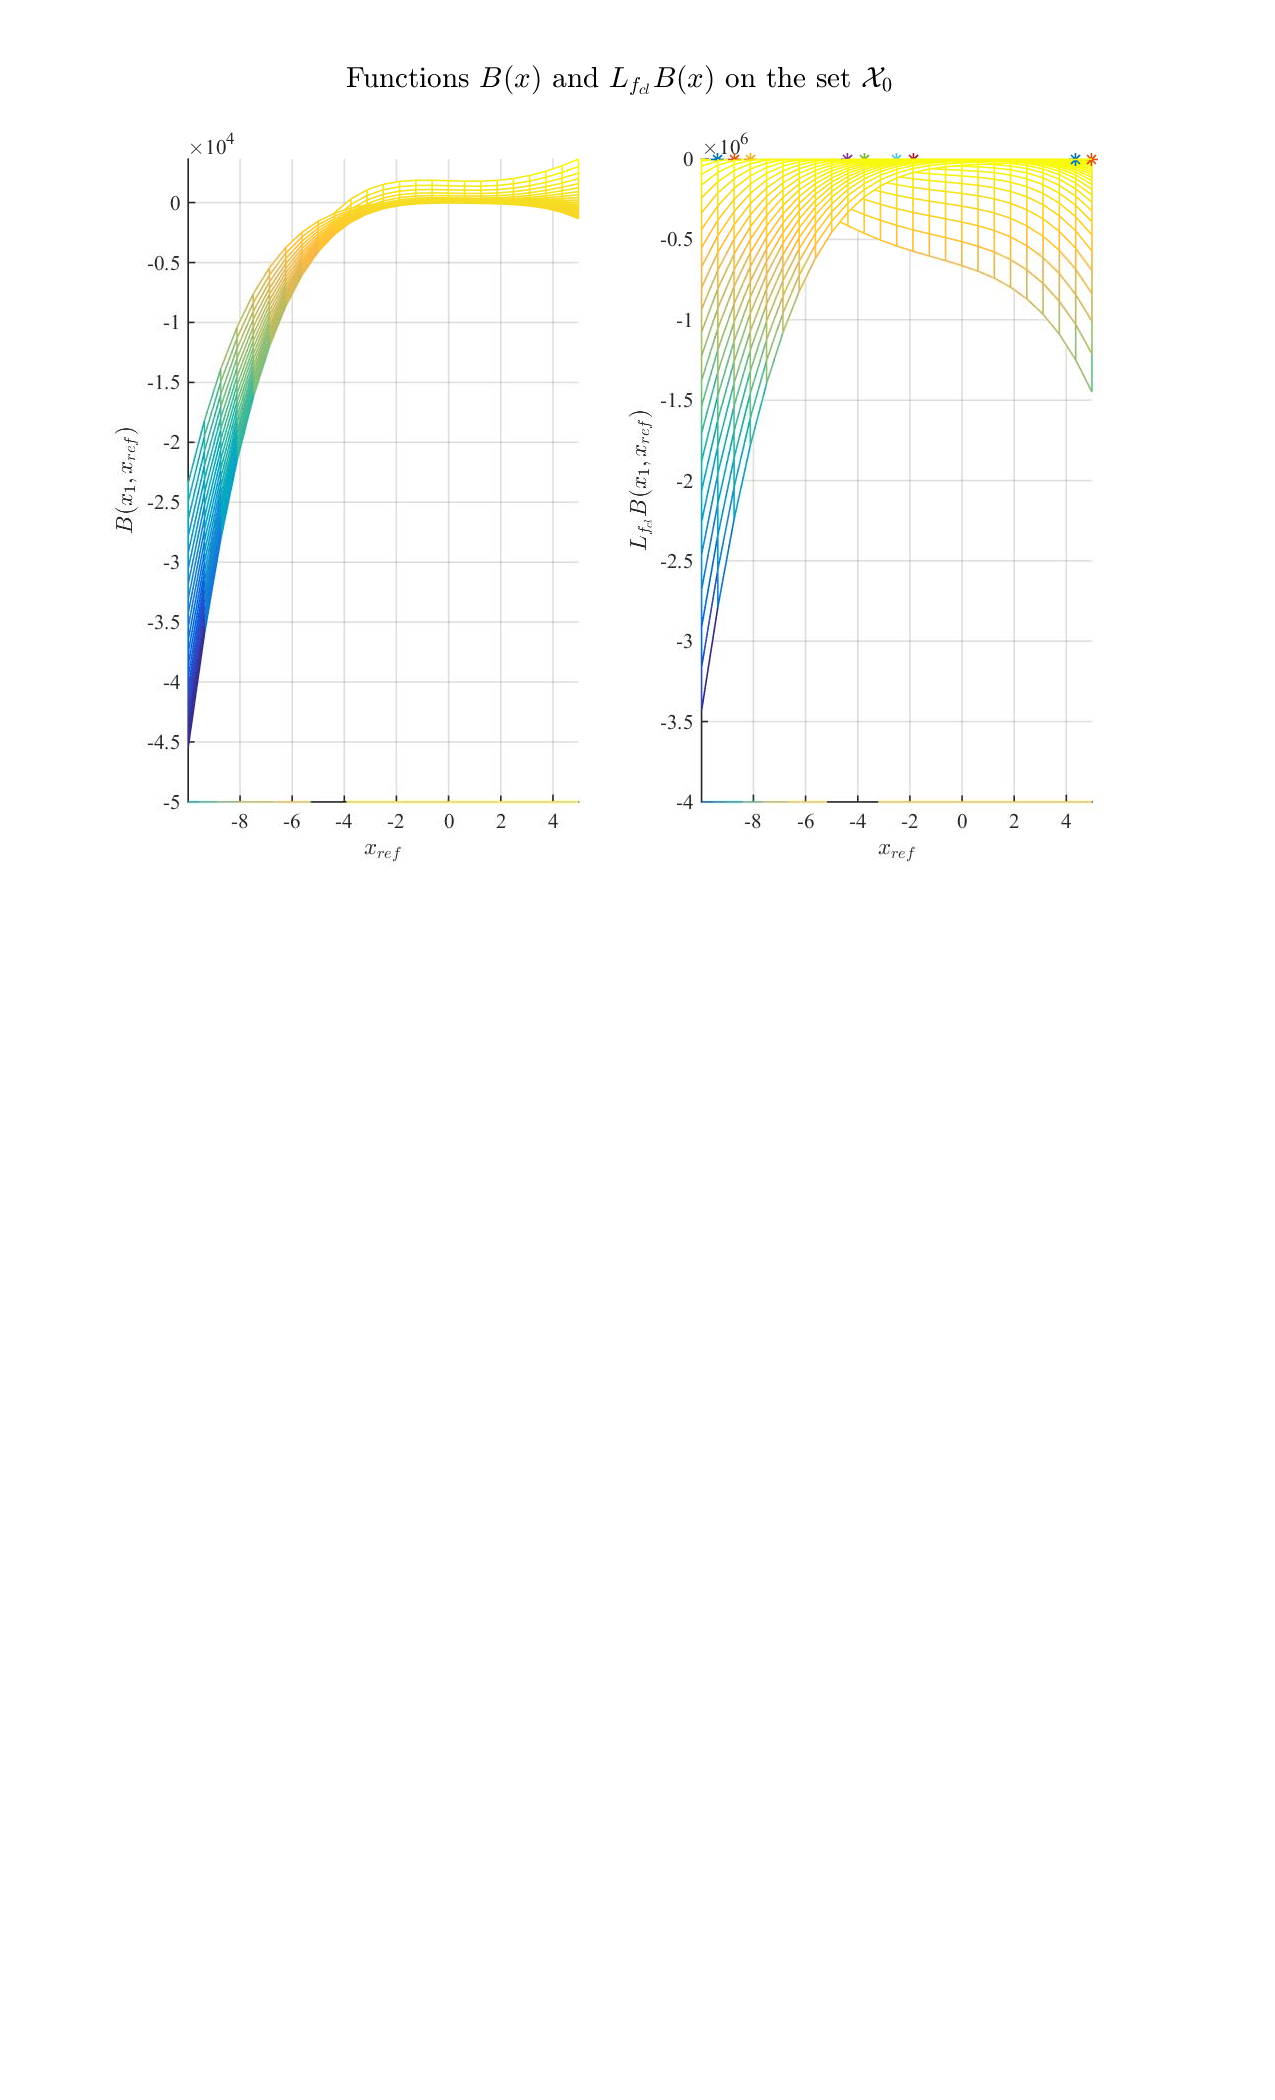
\includegraphics[width=0.5\textwidth]{Bnew1_X0_xref.pdf}}%
\subbottom[]{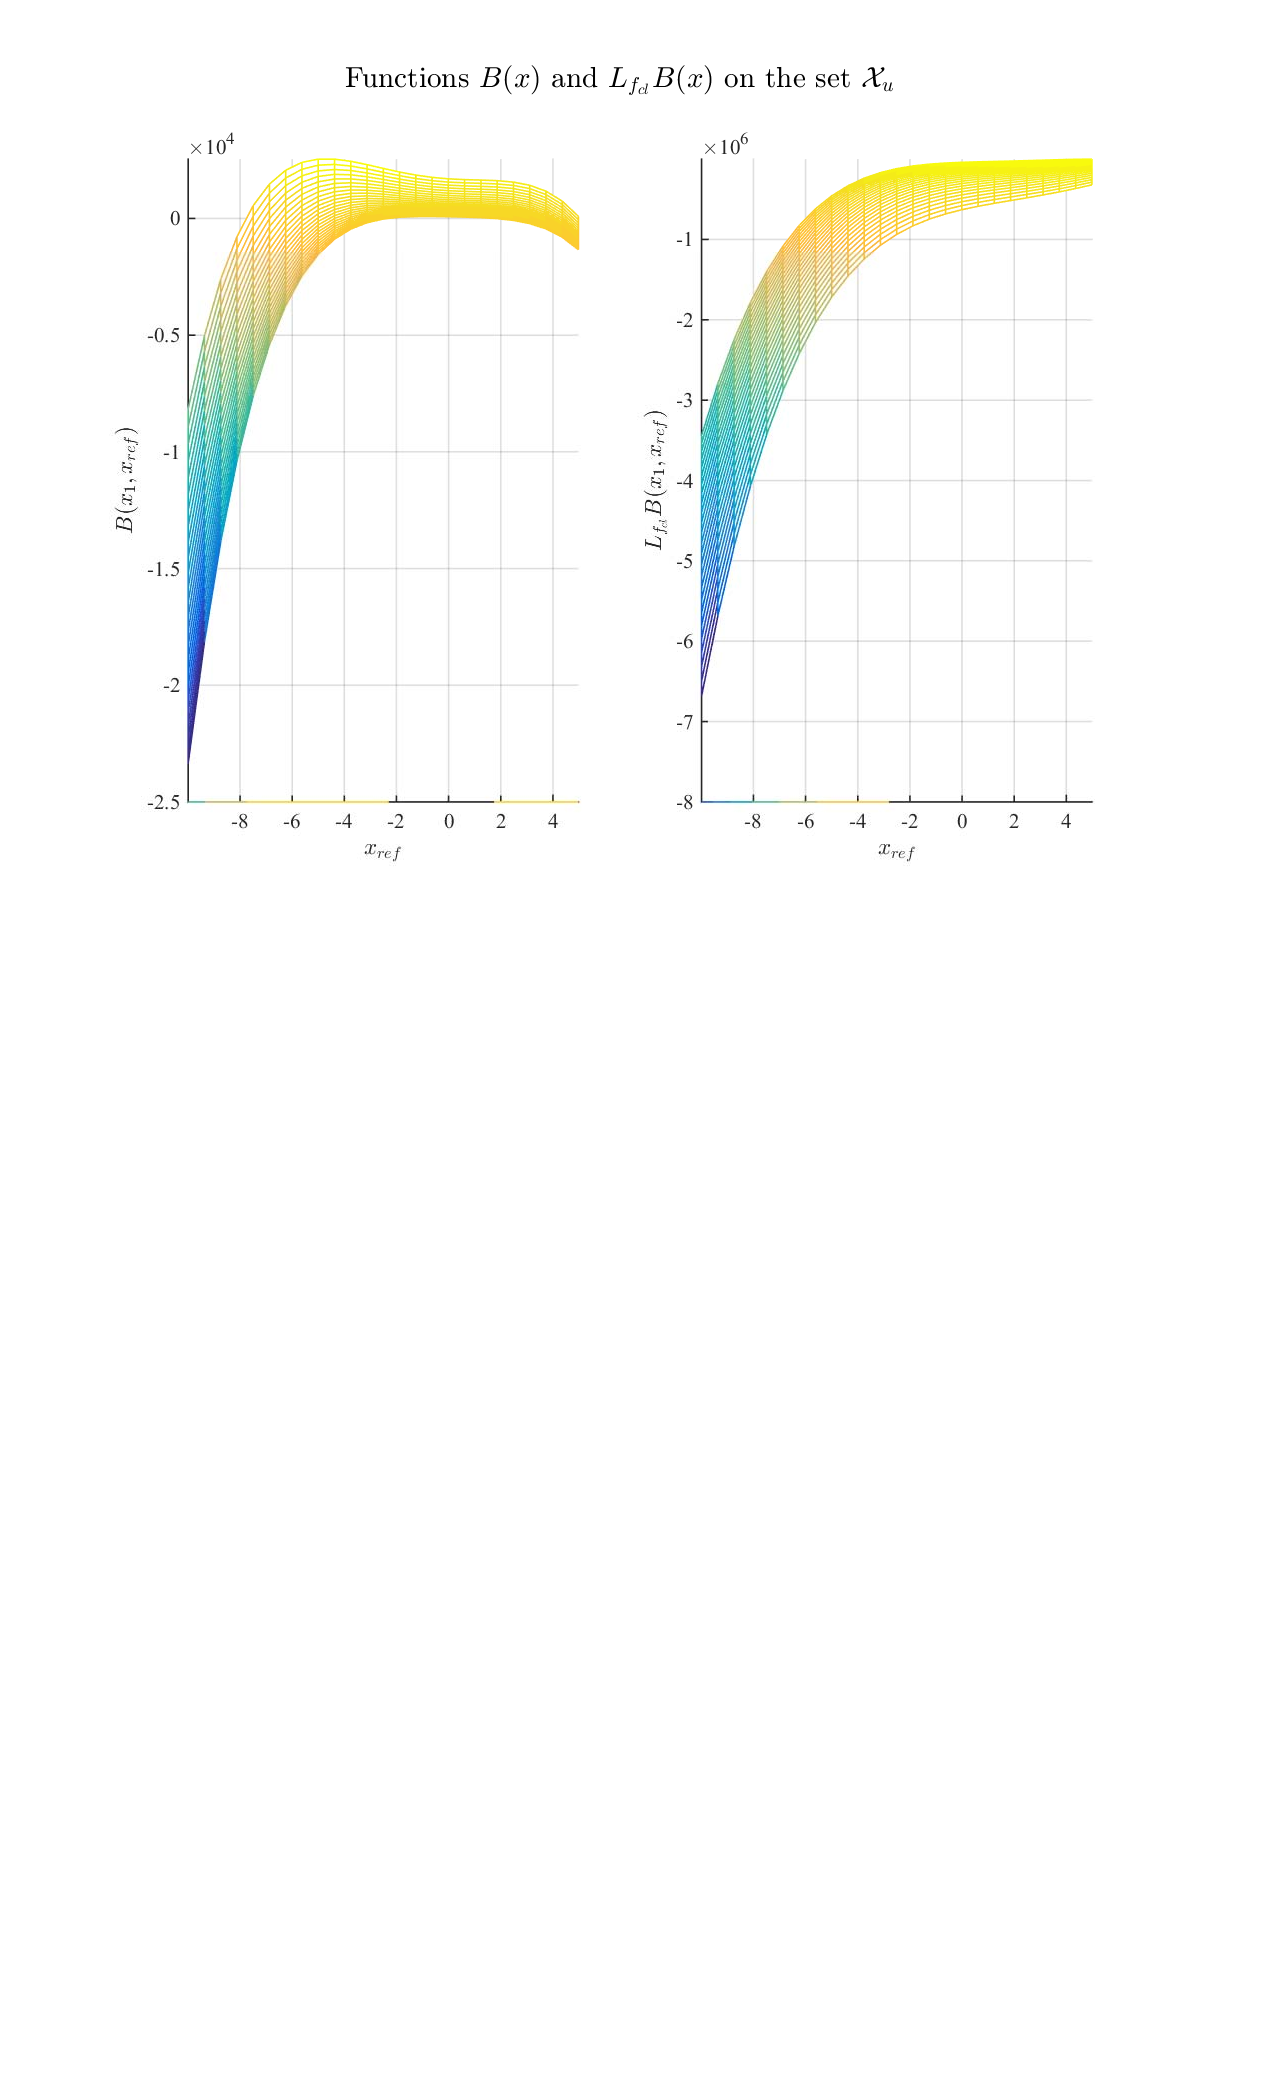
\includegraphics[width=0.5\textwidth]{Bnew1_Xu_xref.pdf}}%
\hspace{1mm}
\subbottom[]{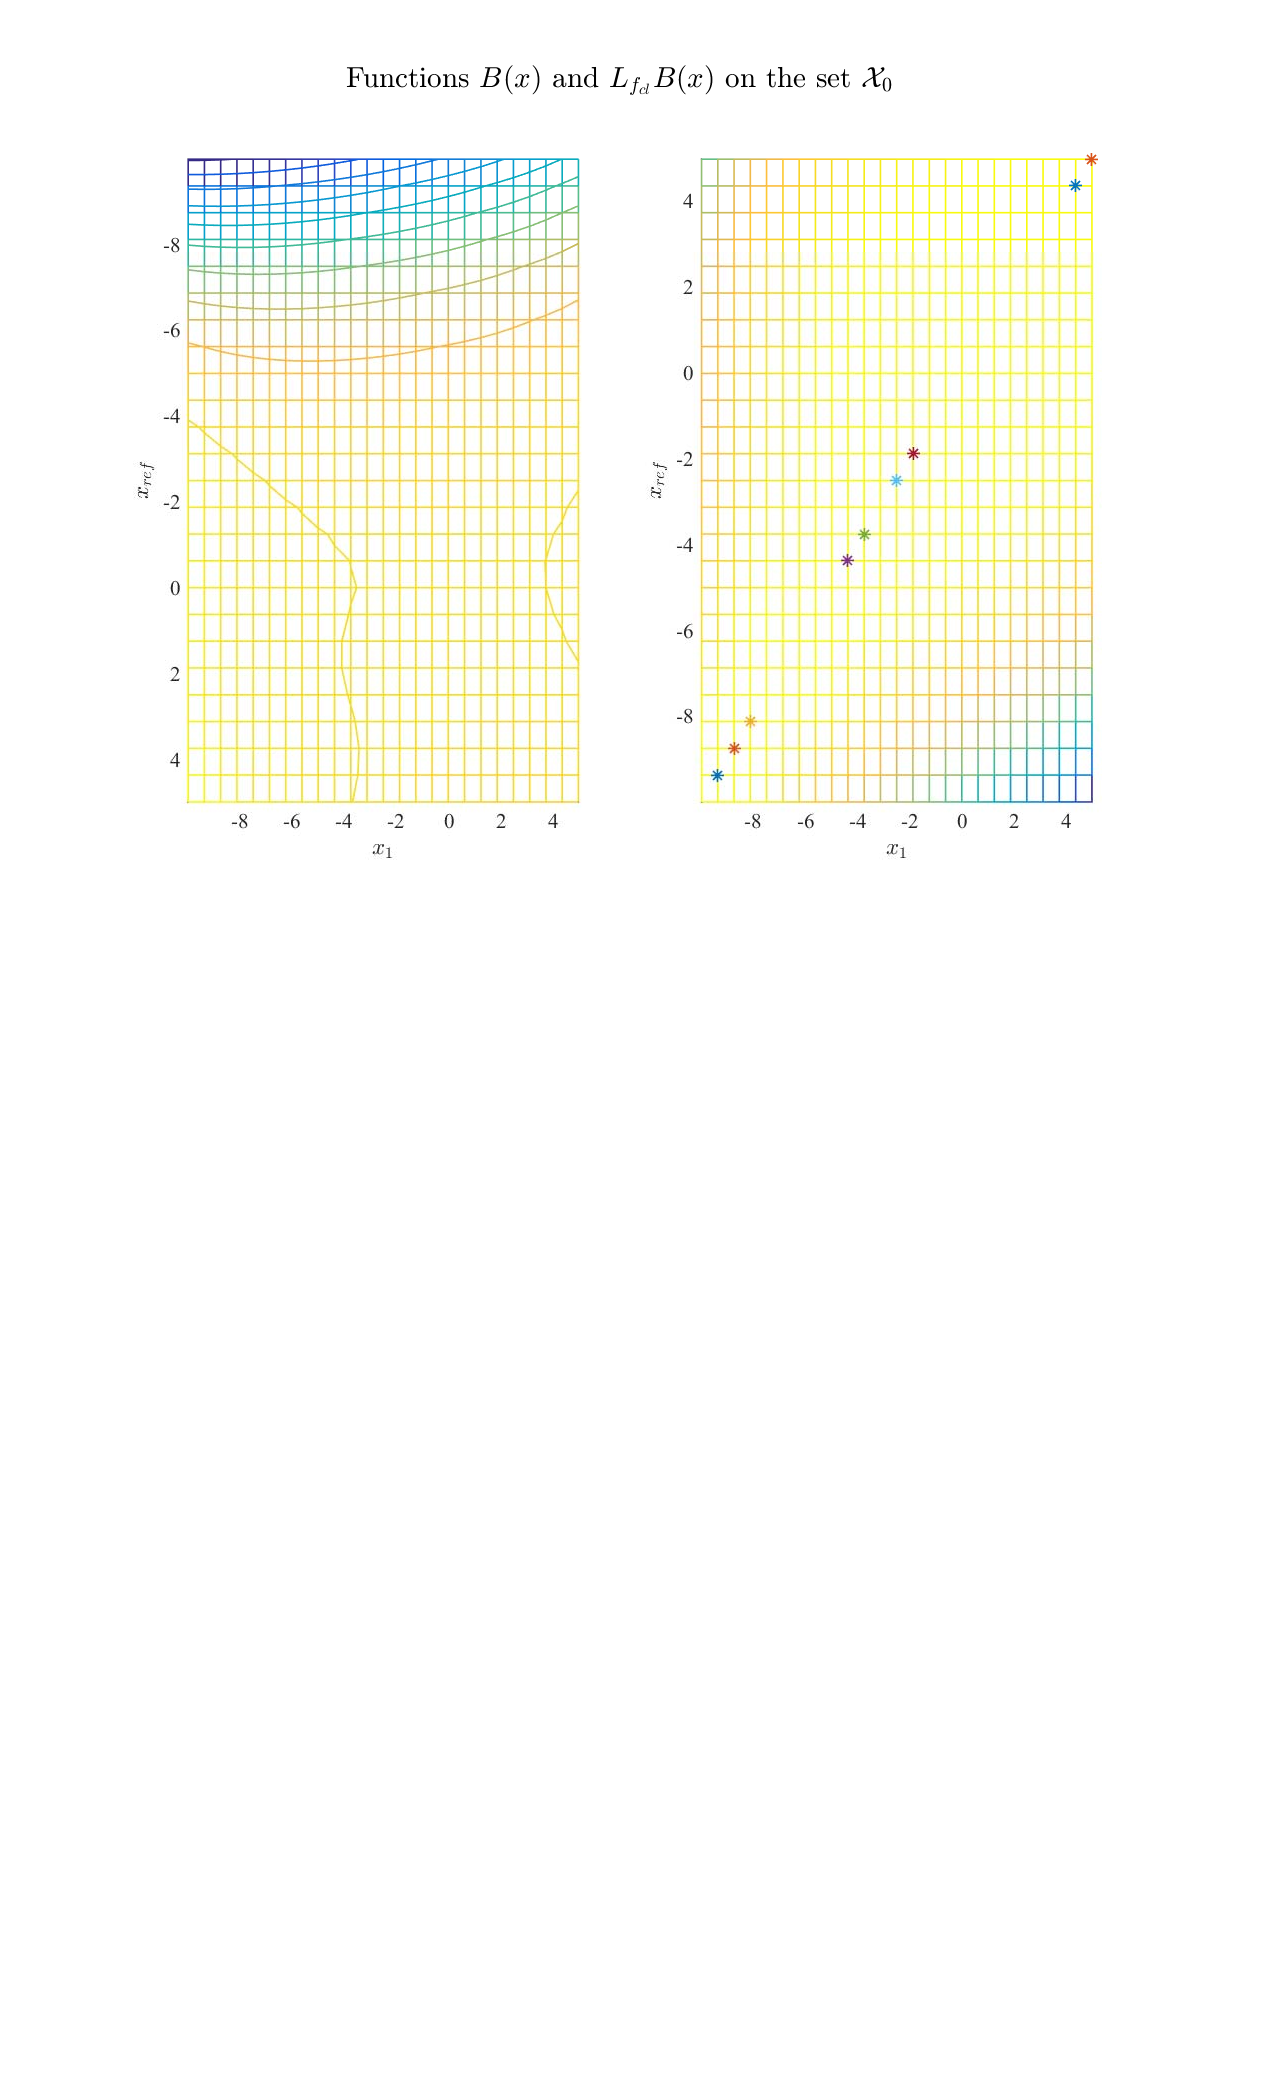
\includegraphics[width=0.5\textwidth]{Bnew1_X0_levelset.pdf}\label{fig:Bnew1_X0_levelset}}%
\subbottom[]{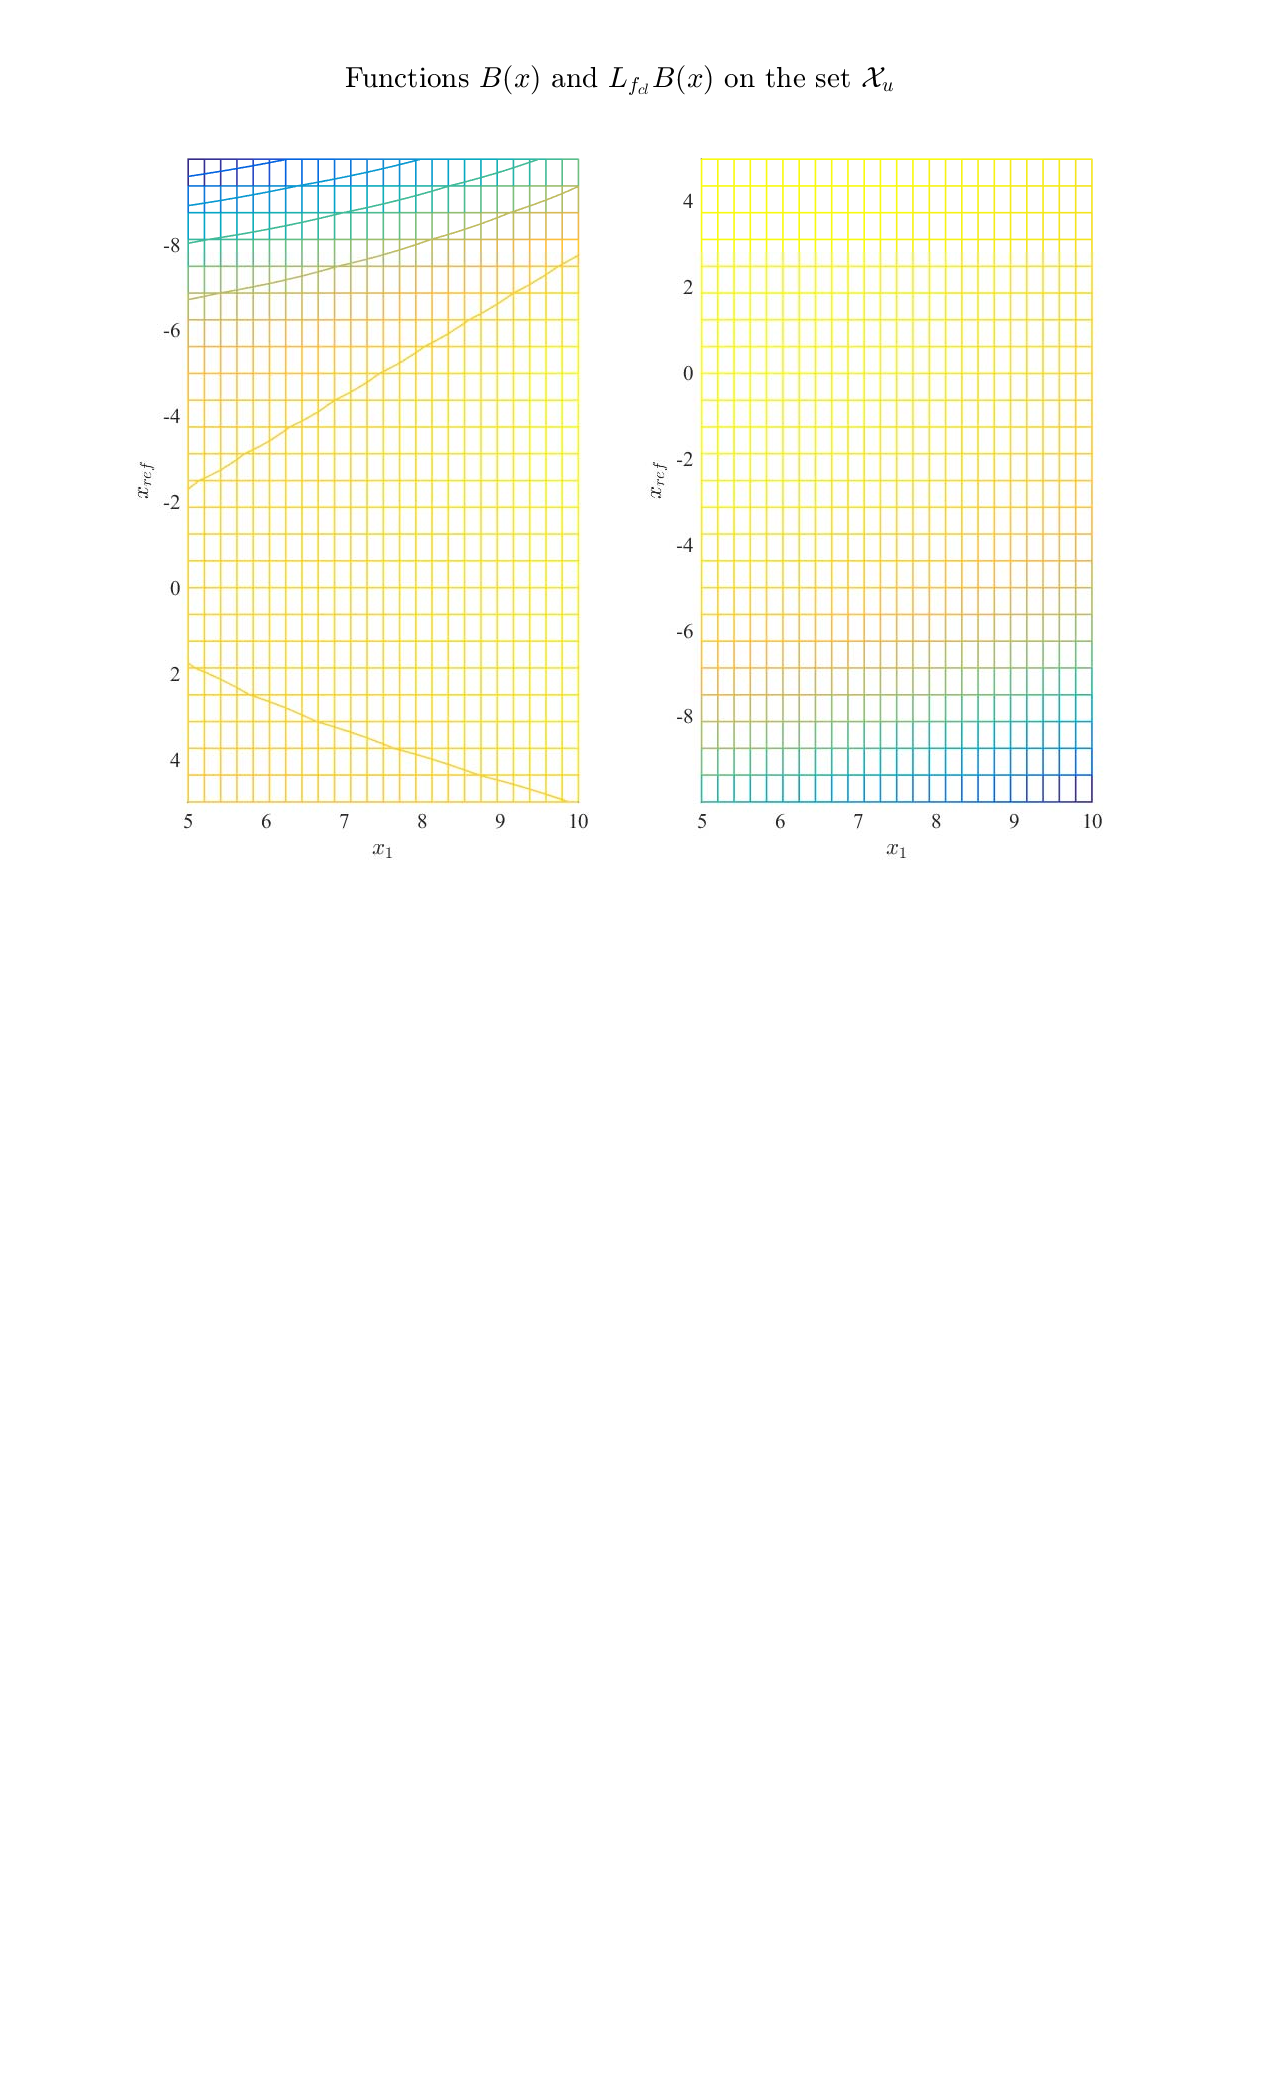
\includegraphics[width=0.5\textwidth]{Bnew1_Xu_levelset.pdf}\label{fig:Bnew1_Xu_levelset}}%
\caption{Left side plots are $B(x)$ and $L_{f_{cl}}B(x)$ on the set $\mathcal{X}_0$, and should all have only nonpositive values. Right side plots are on the set $\mathcal{X}_u$, where $B(x)$ should be positive and $L_{f_{cl}}B(x)$ should be nonpositive. The yellow level sets in \autoref{fig:Bnew1_X0_levelset} and \ref{fig:Bnew1_Xu_levelset} mark the zero level set, and the "stars" in \autoref{fig:Bnew1_X0_levelset} mark points where $L_{f_{cl}}B(x)$ is positive.}
\label{fig:Bnew1}
\end{figure}

In \autoref{fig:Bnew1} the unit of all positions are in centimetres, $\epsilon=1$\,cm (chosen large in order for the numeric error not to cause a wrong solution), $\Delta=0.01$\,cm. Monomials for all SOS $q$-coefficients are set to 0:6, while $B(x_1,x_{ref})$ is of degree 0:4. This setup gives a solution with \texttt{feas.ratio=0.9782}, \texttt{num.err=1}, \texttt{res.norm=2e-5} and leading term coefficient is 1e-1. However, as seen from the plots no feasible solution is found (as $B(x)$ is not nonpositive for the entire set $\mathcal{X}_0$, nor is $B(x)$ positive for the entire set $\mathcal{X}_u$, in fact hardly any of it).

\subsection{Approach the problem backwards}
Trying to decrease the set $\mathcal{X}_0$ (and $\mathcal{X}$) until a feasible solution is found, tweaking $\epsilon$ and $\Delta$ and monomial degrees until all inequalities according to \autoref{eq:barrier_constraints_putinar} are tested to be SOS.

A solution is found for $B(x_1,x_{ref})$ of degree 0:4, monomial degrees are $Z_{X1}$ 0:4, $z_{X2}$ 0:3, $Z_{X_u1}$ 0:4, $Z_{X_u2}$ 0:2, $Z_{X_01}$ 0:2, $Z_{X_02}$ 0:2, with $\epsilon=2$ and $\Delta=0.03$\,cm and with sets as small as (in [cm])
\begin{subequations}\label{eq:sets_case6}
	\begin{align}
		\mathcal{X} &= \begin{bmatrix} 1.6 & 10\end{bmatrix} \times \begin{bmatrix} 1.6+\Delta & 5-2\Delta\end{bmatrix}\\
		\mathcal{X}_u &= \begin{bmatrix} 5 & 10\end{bmatrix} \times \begin{bmatrix} 1.6+\Delta & 5-2\Delta\end{bmatrix}\\
		\mathcal{X}_0 &= \begin{bmatrix} 1.6+\Delta & 5-2\Delta\end{bmatrix} \times \begin{bmatrix} 1.6+\Delta & 5-2\Delta\end{bmatrix}
	\end{align}
\end{subequations}

This solution has a \texttt{feas.ratio=-1.4972} \textcolor{red}{does this mean it is in fact infeasible?}, \texttt{num.err=1}, \texttt{res.norm=5e-4} and leading term coefficient 5e0. The solution is plotted for the two sets $\mathcal{X}_0$ and $\mathcal{X}_u$ in \autoref{fig:Bnew2}.

\begin{figure}[H]
	\subbottom[]{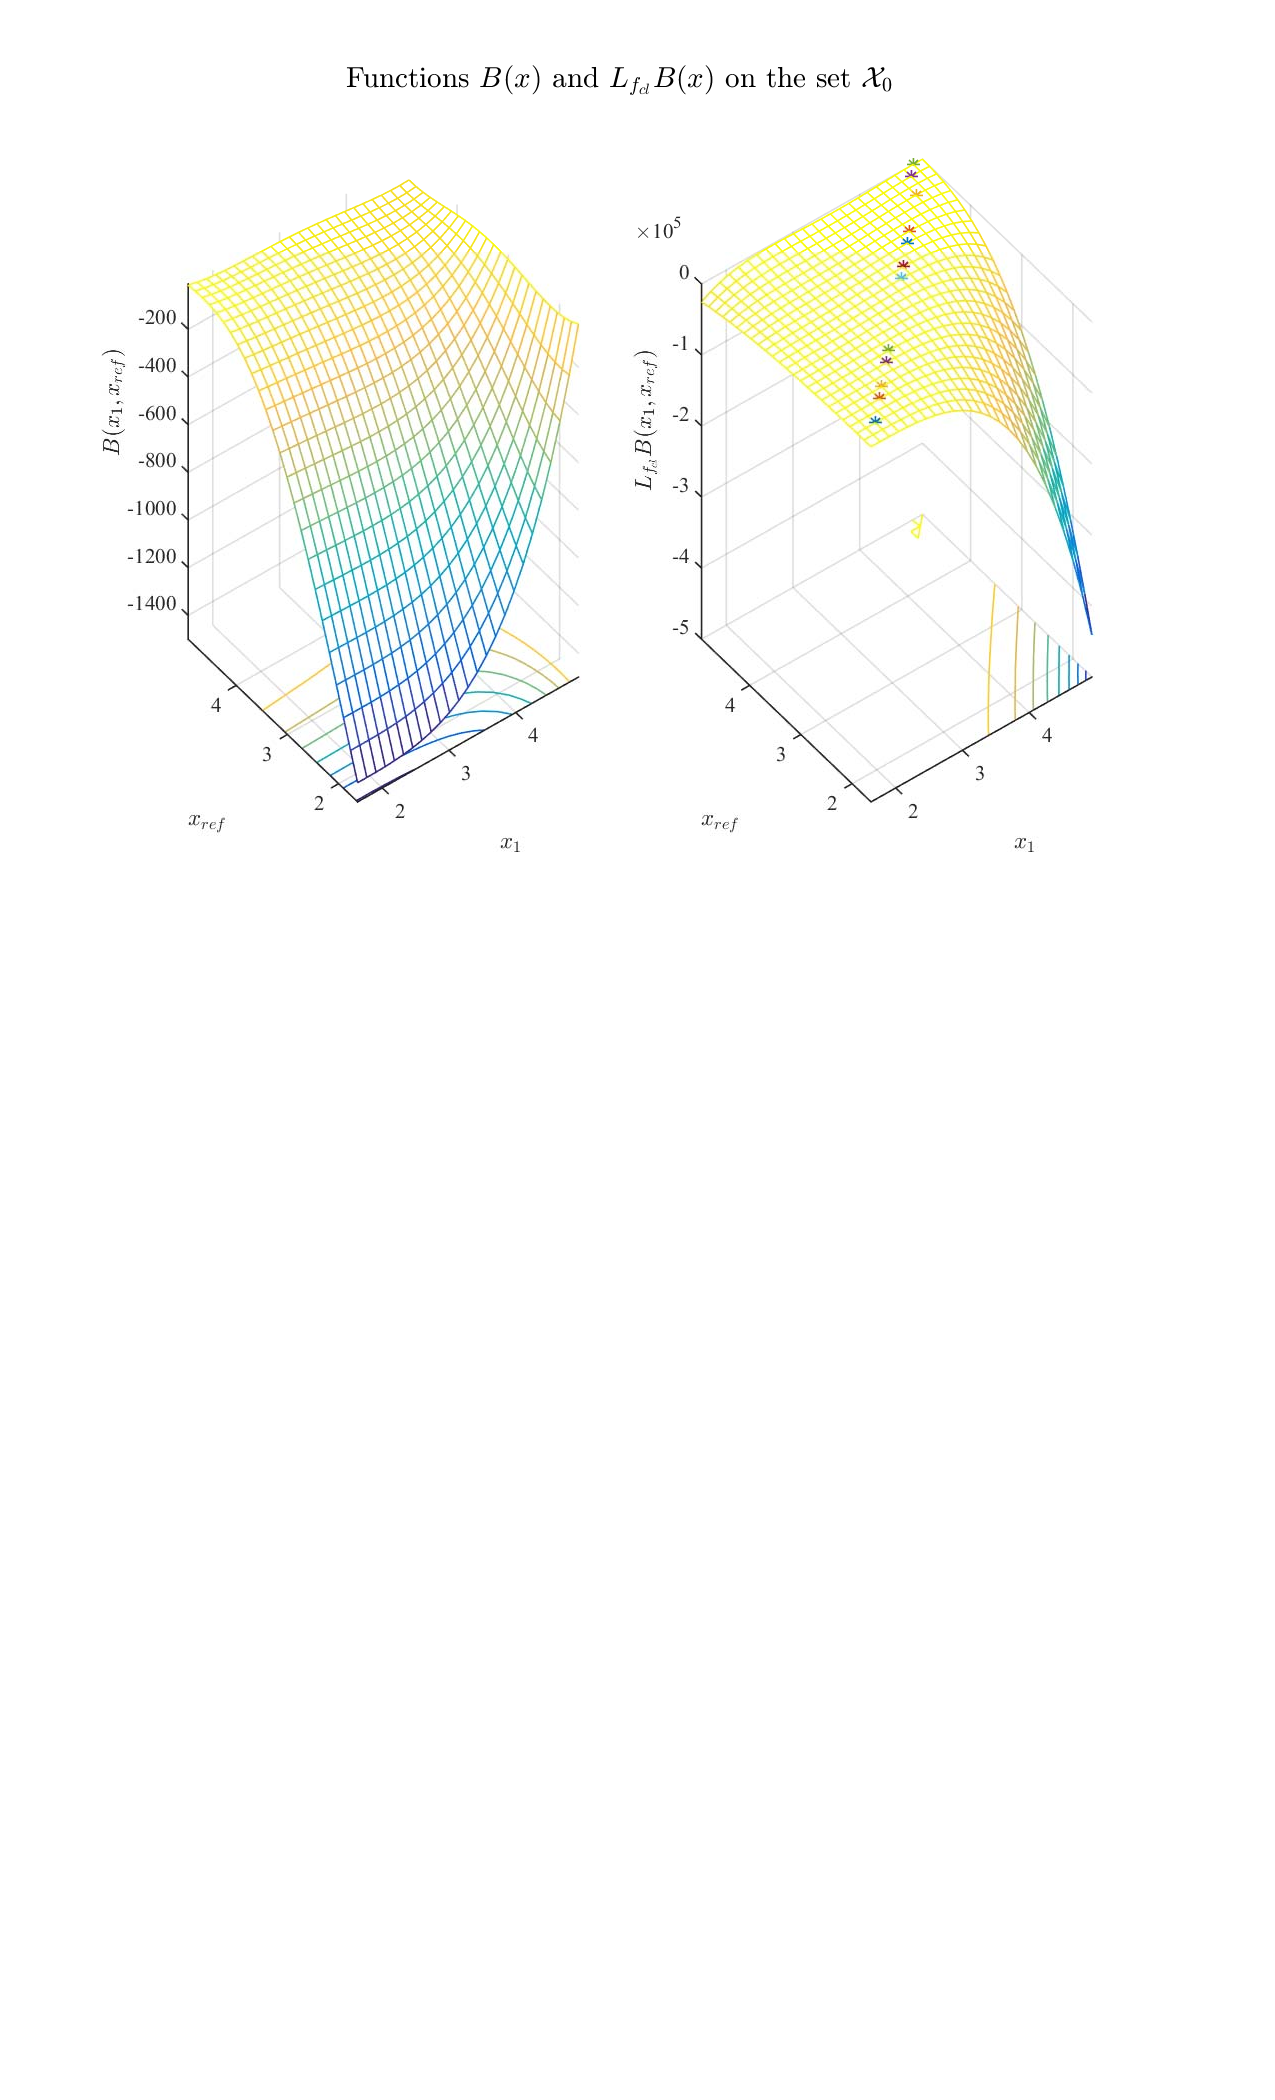
\includegraphics[width=0.5\textwidth]{Bnew2_X0.pdf}\label{fig:Bnew2_X0}}%
	\subbottom[]{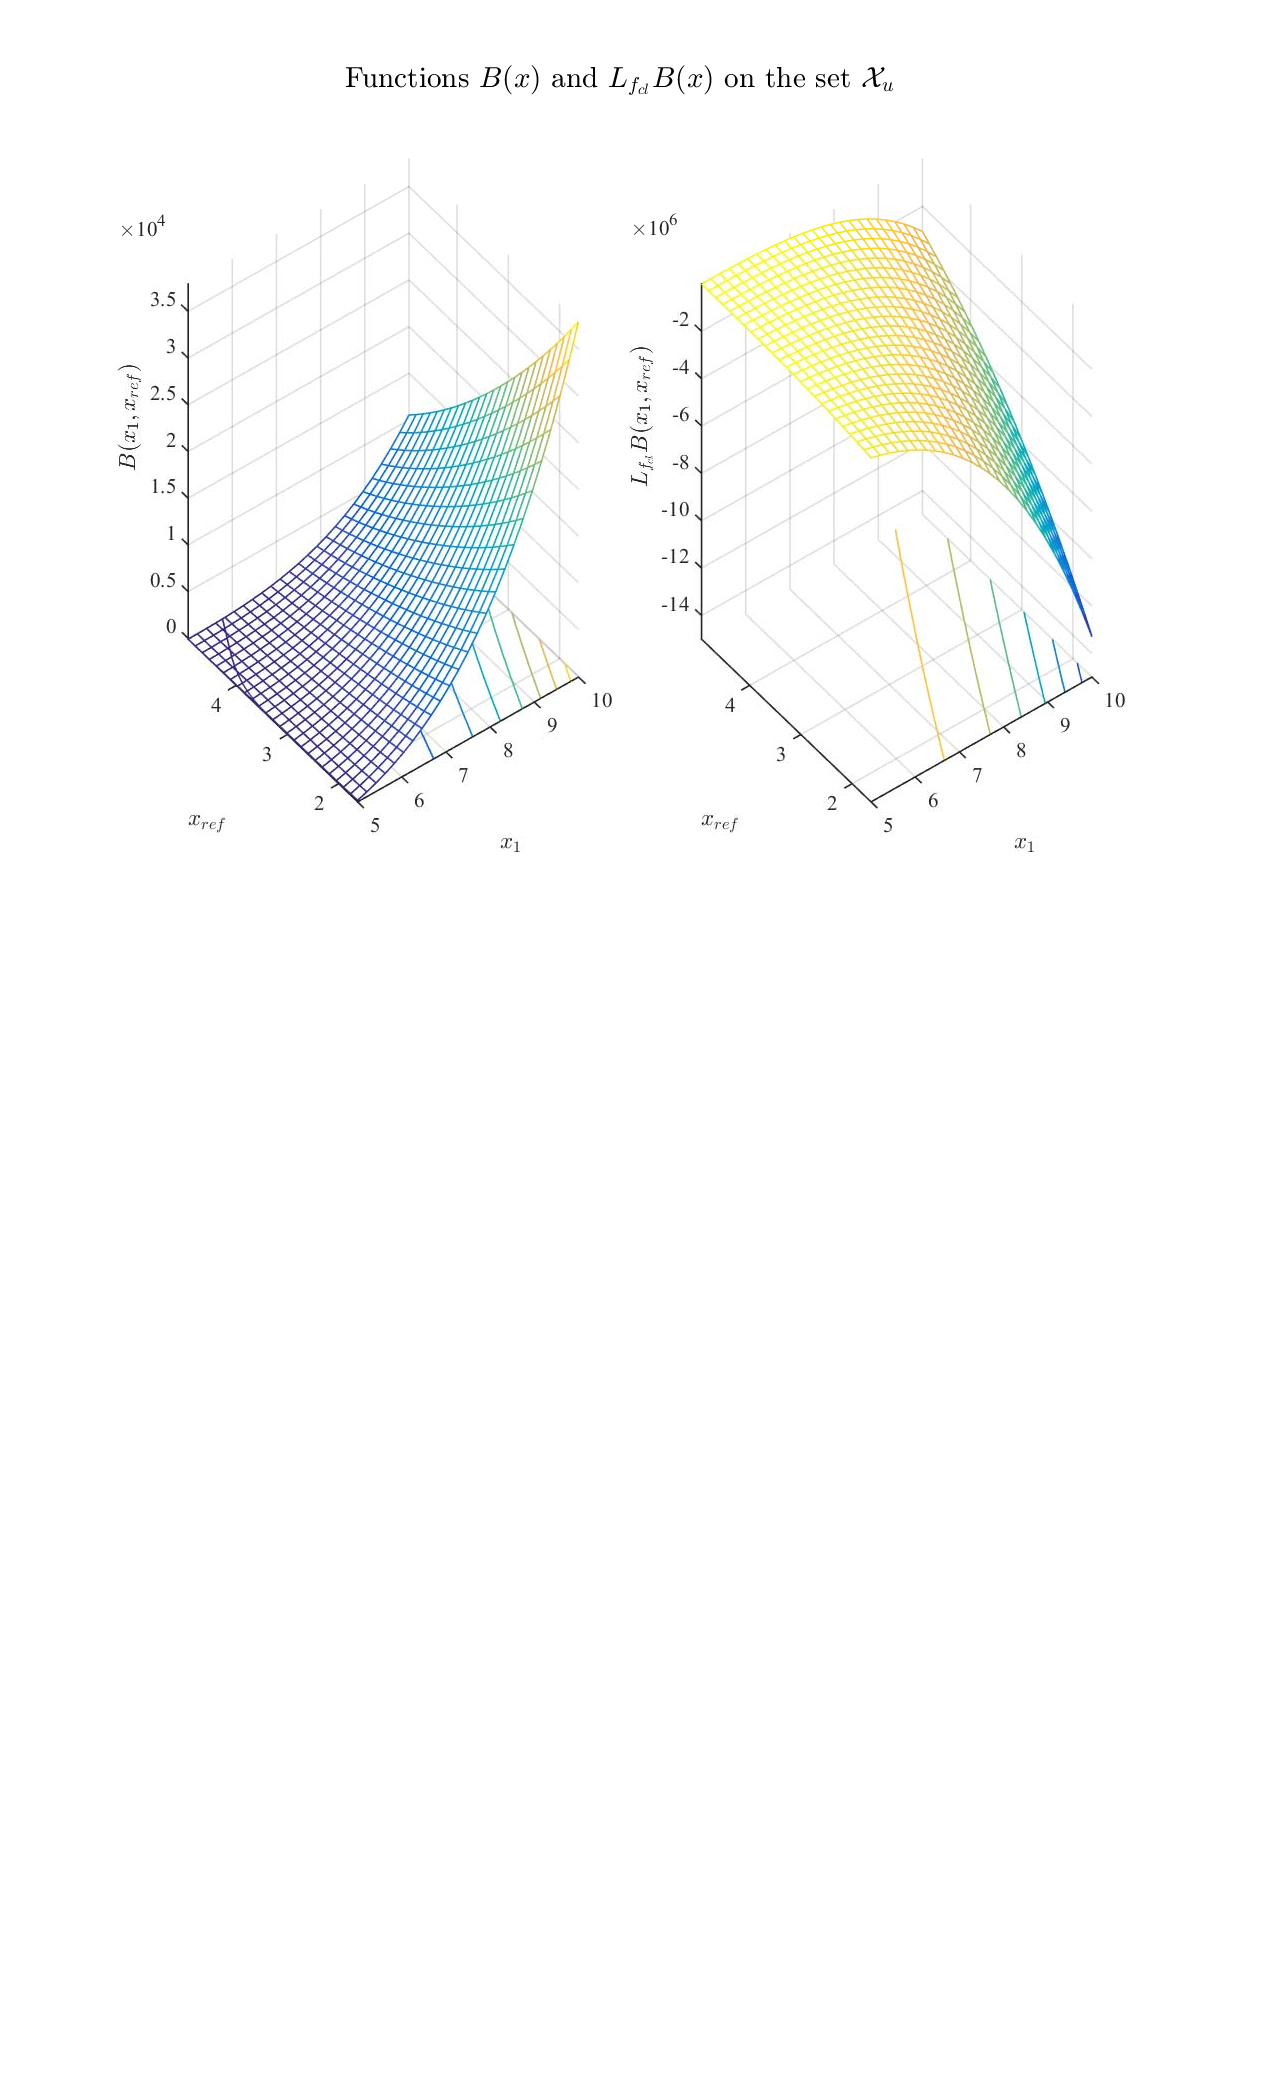
\includegraphics[width=0.5\textwidth]{Bnew2_Xu.pdf}\label{fig:Bnew2_Xu}}%
	\caption{This solution yields a $B(x)$ that is nonpositive on the set $\mathcal{X}_0$ and positive on the set $\mathcal{X}_u$ as desired, and a Lie derivative that is nonpositive \textcolor{red}{(except for $x_1=x_{ref}$)}.}
	\label{fig:Bnew2}
\end{figure}

\newpage
\section{Constructing Barrier Certificate with SOSTOOLS}

Construct the SOS program, with polynomials $g$ such that the sets are defined as in \autoref{fig:sos_Xregion}.
\begin{figure}[H]
	\centering
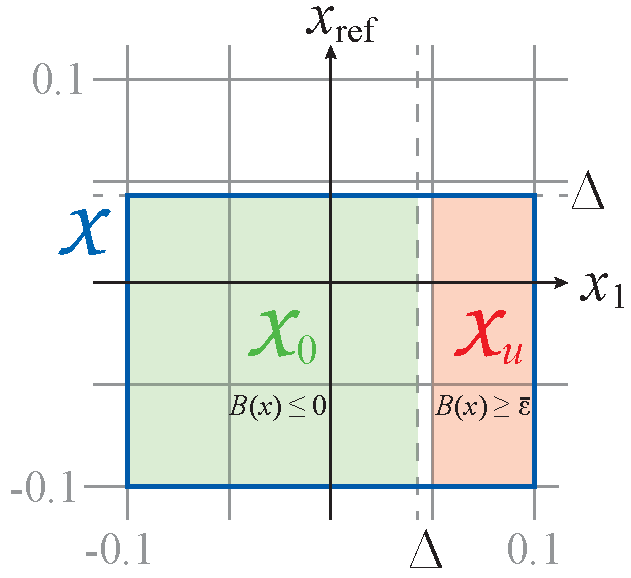
\includegraphics[width=0.4\textwidth]{sos_Xregion.pdf}
\caption{Definition of the sets in the SOS program.}
\label{fig:sos_Xregion}
\end{figure}

\begin{lstlisting}[language=matlab]
prog = sosineq(prog,-[diff(B,x1) diff(B,xref)]*[fx;0]-gX1*qX1 - gX2*qX2);
prog = sosineq(prog,B-epsilon-gXu1*qXu1-gXu2*qXu2);
prog = sosineq(prog,-B-gX01*qX01-gX02*qX02);
\end{lstlisting}

where $g_{\mathcal{X}2}$, $g_{\mathcal{X}_u2}$ and $g_{\mathcal{X}_02}$ are parabola functions of $x_\text{ref}$ all positive on the interval [-0.1,0.05-$\Delta$], and $g_{\mathcal{X}1}$, $g_{\mathcal{X}_u1}$ and $g_{\mathcal{X}_01}$ are parabola functions of $x_1$ positive on the intervals [-0.1,0.1], [0.05,0.1] and [-0.1,0.05-$\Delta$], respectively.

For the first order system described in \autoref{subsec:model_1d} with time constant $\tau=110$\,ms, and with a linear position controller as described in \autoref{eq:utilde}, such that the closed-loop system is
\begin{equation}
\dot{\tilde{x}}=
\dot{\begin{bmatrix}
	x_1\\x_{ref}
	\end{bmatrix}} =
\begin{bmatrix}
-(1+K)/\tau & \bar{N}/\tau\\0&0
\end{bmatrix}
\begin{bmatrix}
x_1\\x_{ref}
\end{bmatrix}
\end{equation}

For the same controller as designed in \autoref{sec:K_Nbar_1D_1storder} with $K=9$ and $\bar{N}=10$, no solution can be found, but for the controller implemented on the da Vinci system with $K=0.2$ and $\bar{N}=1.2$, a solution is found with SOSTOOLS using $\Delta=7.5$\,mm and $\epsilon=1$.

